\documentclass[12pt,a4paper]{report}

%------------------------------------------------------------------------
% PACKAGES:

\usepackage{lmtstyle}
% Define typearea
% a) Use automatic:
\usepackage[BCOR1cm]{typearea}
% b) Or use fixed:
%\usepackage{geometry}
%\geometry{left=1.5cm,textwidth=18.5cm,top=1.5cm,textheight=26.5cm}
\usepackage[american,ngerman]{babel}
% Use list of tabels, etc. in table of contents:
\usepackage{tocbibind}
% German paragraph skip
\usepackage{parskip}
% Encoder:????
\usepackage[latin1]{inputenc}
%\usepackage[applemac]{inputenc}
% Use A4-paper efficiently:
\usepackage{a4wide}
% Index-generation
\usepackage{makeidx}
% Einbinden von URLs:
\usepackage{url}
% Include .eps-files (needed also for the TUM-logo):
%\usepackage{epsf}
% Special \LaTex symbols (e.g. \BibTeX):
\usepackage{doc}
% Include Graphic-files:
%\usepackage{graphics}
% Include Graphic-files:
\usepackage{graphicx}
\usepackage{pdfpages}
% Include doc++ generated tex-files:
%\usepackage{docxx}
% Include PDF links
%\usepackage[pdftex, bookmarks=true]{hyperref}
\usepackage{bbm}
%------------------------------------------------------------------------
\usepackage{natbib}
\usepackage{amsmath}
\usepackage{amsfonts}
\newcommand{\e}{\mathbb E}
\newcommand{\bld}{\boldsymbol}
\graphicspath{{figures/}}
\newcommand{\RNum}[1]{\uppercase\expandafter{\romannumeral #1\relax}}

\usepackage{float}
\floatstyle{plaintop}
\restylefloat{table}
%\usepackage[tableposition=top]{caption}
%\usepackage{placeins}
%########################################################################
% CHOOSE DEFAULT LANGUAGE:
\setlang{en}
%\setlang{de}

% FILL IN ACCORDINGLY:
\title{Uncertainty-Based Improvement of a Visual
	Classification System}
\type{M} % / M:Master /B:Bachelor / F:Forschungspraxis / I:Ingenieurspraxis
\author{Jianxiang Feng}
\matrikelnr{03679926}
\street{Connollystr. 03/W06	}
\town{80809 Munich}
\advisor{Prof. Dr. -Ing. Eckehard Steinbach}
\supervisor{ Dr. Zolt�n-Csaba M�rton, Maximilian Durner}
\datebegin{11.10.2018} %11.10.2018
\dateend{25.04.2019}
%########################################################################


\begin{document}%****************************************************
\makemtgtitle

% MAIN PART:
\pagenumbering{roman}
% German abstract:
% \switchlanguage{de} % The Kurzfassung, if given, is supposed to be in German!

\thispagestyle{plain}

\section*{Kurzfassung} 
In der Kurzfassung werden auf einer halben Seite das Problemfeld und
die pr�sentierten Ergebnisse zusammengefasst.

\switchlanguage{\lang} % Switch back to the docmuent's default language.
% English abstract:
\switchlanguage{en} % The abstract is supposed to be in English!

\thispagestyle{plain}

\section*{Abstract}
%Deep learning based classifiers have achieved tremendous success on different tasks. However, this kind of classifier cannot provide reliable uncertainty estimation about their predictions and express excessive overconfidence, which means that the models are highly certain although they are not familiar with the related input. This behavior can easily lead to severe consequences in safety-critical applications such as diagnosis of diseases, perception of self-driving car and so on. Especially in the case of the deployment of robots, the robots should be aware of the correctness of the predictions they make, so that they are able to avoid unnecessary accidents and adapt itself in an unfamiliar environment. Besides uncertainty for independent data examples, uncertainty related to dependencies between data examples should be taken into account. When recognizing objects with similar appearances but different contexts in a specific scene, the classifier should express reliably high uncertainty about its predictions because of appearance ambiguities. At the same time, contextual information should be handled properly and utilized to resolve this kind of ambiguities, aiming to further improve the performance. 

%In this work, Bayesian neural networks with different inference techniques such as dropout variational inference and scalable Laplace approximation are employed to improve the uncertainty estimation. With a reliable uncertainty estimation, a classifier trained on an easily obtainable dataset should be able to adapt itself in a test environment by collecting dataset for fine-tuning with as little manual efforts as possible. Additionally, a conditional random field is employed to further improve the performance by utilizing more information brought by better uncertainty estimation and handling the contextual information between objects properly. Extensive experiments are performed to show that uncertainty estimation can be improved with Bayesian neural networks in terms of different evaluation metrics. Besides, it is demonstrated that manual efforts in collecting dataset for fine-tuning a classifier can be reduced with the help of improved uncertainty estimation on experiments with two different datasets. Last but not least, experiments also show that the conditional random field is able to further improve the performance by making use of better uncertainty estimation and contextual information.

Deep learning based classifiers have achieved tremendous success on different tasks. 
However, this kind of classifiers cannot provide a reliable uncertainty estimation and express excessive overconfidence, which means that the models are always highly certain even on unfamiliar data.
This behavior can easily lead to severe consequences in safety-critical applications such as diagnosis of diseases, perception of self-driving car or robotics. 
Robots should be aware of the correctness of their predictions to prevent unnecessary accidents and/or to detect failure cases.
Furthermore, this kind of introspection can help the robot to recognize unfamiliar environments and to adapt gradually.
%Besides uncertainty for independent data example, uncertainty related to dependencies between data examples should be taken into account.
However, uncertainties of independent data examples do not take into account uncertainty related to dependencies between data examples.
% cannot be captured straight-forward and additional information has to be incorporated.
Given a classifier with good uncertainty estimations the classification of objects with similar appearances should result in a high uncertainty about its prediction due to the appearance ambiguity, which can still lead to miss-classification. To overcome this issue, contextual information can be used to resolve the ambiguities and improve the initial prediction.

In this work, the uncertainty estimation of deep neural networks are improved by employing Bayesian neural networks. 
Within this context the applicability and performance of different inference techniques such as dropout variational inference and scalable Laplace approximation are evaluated.
The resulting network is applied to a continuous learning use-case where the improved uncertainty estimation is used to select data samples for fine-tuning in an interactive (automatically and manually labeling) manner.
For further improvements a conditional random field is employed to fuse the initial predictions with contextual information between objects.
%Additionally, conditional random field is employed to improve the performance further by utilizing more information brought by better uncertainty estimation and handling the contextual information between objects properly. 
Extensive experiments are performed to show that the uncertainty estimation can be improved with Bayesian neural network in terms of different evaluation metrics.
Besides, it is experimentally shown that manual efforts for collecting a dataset for fine-tuning a classifier can be reduced with the help of improved uncertainty estimation on two benchmark datasets. 
Last but not least, experiments also show that the conditional random field is able to further improve the performance by incorporating contextual information.

\switchlanguage{\lang} % Switch back to the document's default language.

% Table of contents:
\tableofcontents 

% Introduction (Einleitung):
\chapter{Introduction}
\pagenumbering{arabic}%Ab hier, werden arabische Zahlen benutzt
\setcounter{page}{1}%Mit Abschnitt 1 beginnt die Seitennummerierung neu.
\thispagestyle{empty}

\section{What is uncertainty?}
This question seems a little philosophical and difficult to answer. However, in the context of modeling in machine learning, I find one answer reasonable and illustrative, that is "Uncertainty arises because of limitations in our ability to observe the world, limitations in our ability to model it, and possibly even because of innate nondeterminism."\cite{koller2009probabilistic}. In spite of innate nondeterminism, uncertainty can be further categorized into two main types :\textbf{epistemic uncertainty} and \textbf{aleatoric uncertainty} \cite{der2009aleatory}\cite{senge2014reliable} \cite{kendall2017uncertainties}. 

The former one, epistemic or model uncertainty illustrates the uncertainty in modeling, which is associated with \textbf{imperfect models} of the real world because of insufficient or imperfect knowledge of reality, which corresponds to our ability of modeling, and thus refers to uncertainty caused by a lack of knowledge, i.e., it refers to the epistemic state of the decision maker. Therefore it may be reduced through collecting more knowledge. Examples for this kind of uncertainty can be uncertainty of model parameter, or uncertainty of model structure depending on which kind of model and so on. One simple example to illustrate this kind of uncertainty would be linear regression with limited observed points, where we can use different curves to explain those points and then predict unobserved points with those curves. If we have observed enough points in some intervals, the models or curves that are able to explain the data are more restricted and if there are not enough points, there would be more curves that can explain these points, which indicates high uncertainty. In reality, it's quite normal to have inadequate data, and thus difficult to model the underlying distribution quite well and precisely. Therefore we could explain the data with several or many different models, where the model uncertainty comes in.

The latter one, aleatoric or data uncertainty, accounts for the \textbf{inherent randomness} of underlying phenomenon which is expressed as variability in observed data and meanwhile associated with the limitation of our observing ability. It's treated as non-reducible within our ability to observe the data. Examples for this kind of uncertainty could be noise induced by limited resolution of sensor or ambiguity from content of data which are unrelated to the model we use to represent these data. One example can be classification of images captured by cameras with different resolutions, images with lower resolutions would have higher uncertainty because they are more ambiguous and less illustrative compared with those with higher resolutions. 

In other words, epistemic uncertainty refers to the reducible part of the (total) uncertainty, whereas aleatoric uncertainty
refers to the non-reducible part. Model uncertainty and aleatoric uncertainty are combined and expressed in the final prediction, which is so called predictive uncertainty.

\section{Why do we need uncertainty?}
Aforementioned model uncertainty represents the belief of model about its predictions and thus bring us more useful information about predictions related with model and observed data instead of just a crispy prediction, whose predictor, is always overconfident when advanced neural network architectures are employed\cite{guo2017calibration}. As far as I am concerned, this kind of uncertainty plays an important role in two following scenarios. 

The first one are those requiring \textbf{high safety guarantee} or \textbf{optimal decision-making}, in which false predictions can cause hazardous consequences, which is so called AI safety\cite{amodei2016concrete}. With reliable model uncertainty estimation, we are able to know when the model is uncertain about its prediction and then people or operator are aware of that and can take corresponding counter measures in order to avoid unnecessary accidents. With more and more wide-spread deep learning algorithms in real life applications, concrete examples for this case include steering control in self-driving car\cite{mcallister2017concrete}, disease diagnosis in medical domain\cite{leibig2017leveraging}, or even tasks in aerospace or other domains requiring higher precision and stronger robustness and so on. Although someone would argue that if the trained model can perform perfectly, that means that it is able to achieve 100\% accuracy, then we do not need this kind of uncertainty information. However, as mentioned in \cite{denker1991transforming}, it's hard or even impossible to have enough training data to define a precise model, which is in coincidence with reality because it's hard to define a task very precisely and get access to enough samples drawn from its real distribution. Uncertainty information would be more valuable and important when algorithms are confronted with multiple tasks\cite{kendall2017multi}. Other relevant tasks such as misclassified and out-of-distribution data detection\cite{hendrycks2016baseline} and adversarial attacks \cite{kurakin2016adversarial}\cite{feinman2017detecting} have also attracted more and more research interests in uncertainty estimation in order to address these challenges.

The second one are scenarios requiring \textbf{interaction between algorithms and people or environments}. Model uncertainty can build a bridge between machine learning algorithms and human beings which can construct a more robust and more data-efficient machine learning system. This scenario involves different kinds of tasks such as active learning\cite{gal2017deep}, reinforcement learning\cite{blundell2015weight}\cite{osband2016deep}\cite{gal2016improving}, automatically labeling, industrial components inspection and so on. The idea behind that is, with reliable model uncertainty estimation we know which data sample or prediction the model is unfamiliar with. In active learning or reinforcement learning, those unfamiliar data samples can be used to train our model more quickly and efficiently. In tasks involving human robot interaction, we can know when the model requires help from human experts based on uncertainty estimation. For example, in industrial component inspection task, we firstly train a model which can perform quite well on some evaluation datasets and then deploy them in real applications. At this moment, we assume that all predictions made by the model are true all the time. However, there is no guarantee that this model has learned to represent the real distribution of data perfectly and is robust against slight or even large domain transfer. If the distributions of the real world data vary because of unexpected factors such equipments aging or changes of weather condition. The model would fail silently and lead to unexpected accidents. With reliable model uncertainty estimation, this kind of weakness can be mitigated or even eliminated. 

On the other hand, aleatoric uncertainty mainly assist in \textbf{improving model performance} by quantifying and considering this kind of information by representing noisy level of predictions and making good use of data points with less noise. By taking this information into account, the model can be trained more optimally and yield better performance, some examples of image data and Lidar data can be referred to \cite{kendall2016modelling}\cite{feng2018towards}. Instead of representing noise, data uncertainty also includes uncertainty from semantic view point, which we can also incorporate into training and yield more robust model. This kind of uncertainty is not quantified explicitly but can be incorporated conceptually with help of specifically designed model and high level statistics cues or features to \textbf{disambiguate prediction} directly. One example of this can be modeling contextual information among pixels with conditional random field in semantic segmentation task\cite{krahenbuhl2011efficient}\cite{sutton2012introduction}\cite{lin2016efficient}. The idea behind that is simple and conditional random field provides a principle way to achieve this idea. Since uncertainty caused by appearance ambiguity represents strong correlation between different categories. Conditional random field can model correlation or dependency between random variables by taking into account high order potentials. In semantic segmentation task, because of the reason of tractable computation, at most second order potentials are taken into account and can yield better performance compared results with just first order potentials.

\section{How can we obtain and handle uncertainty in deep learning?}
As we know, deep learning is a powerful black box model while it has achieved tremendous success in different tasks. Therefore to obtain and handle uncertainty in deep learning model and data can help us to get more understanding about this black box model and make deep learning based application more robust and safer. 

Regarding model uncertainty or quality measure that acts similar to model uncertainty, there are many different ways to obtain this kind of quality measure of prediction. On the one hand, because of intractability of real model uncertainty in deep neural networks, there are some \textbf{ad-hoc approaches} that try to obtain such a quality measure on specific tasks which are solved usually with model uncertainty such as misclassified and out-of-distribution(OOD) detection task. \cite{liang2017enhancing} combines temperature scaling and input preprocessing which is called adversarial training together and yields a simple but effective out-of-distribution sample detector, but this approach requires additional out-of-distribution dataset for training which is hard to collect in reality. \cite{devries2018learning} modifies the loss function to train a classifier against OOD data, however this approach is hard to generalize in case of slight domain transfer. \cite{lee2017training} treats uniform distribution as ground truth distribution of OOD data and show that OOD data can be generated via generative adversarial network(GAN). This approach seems practical, but training GAN effectively does not always work for images of large size because of high dimension of data distribution. 

On the other hand, there are some more theoretically sound approaches which employ \textbf{Bayesian neural network}\cite{mackay1992practical}\cite{neal2012bayesian}, \textbf{bootstrap}\cite{osband2016deep} or \textbf{ensemble} method\cite{lakshminarayanan2017simple} or even ensemble of Bayesian neural network\cite{smith2018understanding}. Although Bayesian neural network provides a principal way to obtain model uncertainty by putting randomness on model parameters, it's difficult to infer the exact posterior distribution over model parameters of deep neural network because of its complex architecture and large scale dataset. Therefore approximate inference plays an important role in addressing this issue. The golden standard for approximate inference is Hamiltonian Monte Carlo\cite{neal2012bayesian}, which requires dealing with whole batch training data and storing the samples of posterior distribution. While the former issue is addressed partially by stochastic gradient Langevin Dynamics\cite{welling2011bayesian}, the latter one attracts many research interests like \cite{balan2015bayesian}\cite{wang2018adversarial}. However, since it's a Markov Chain Monte Carlo(MCMC) method, to assess the convergence is still non-trivial.
 
There are some alternatives to MCMC, one popular one is variational inference(VI)\cite{hinton1993keeping}. In VI, this inference problem is cast into optimization problem by minimizing the Kullbach-Leibler divergence between the approximate posterior distribution and real posterior distribution. Therefore approximate distribution family needs to be chosen and thus has a large impact on the result, which may impede the performance if the chosen distribution family is not flexible enough for the problem. \cite{graves2011practical} firstly employed fully factorized Gaussian with a biased gradient estimator on a practical problem. Later \cite{blundell2015weight} improved the result with the same approximate distribution but different estimator with help of "reparameterization trick"\cite{kingma2013auto}. \citealp{hernandez2015probabilistic} also used the same approximate distribution but with expectation propagation\cite{minka2001expectation} instead of VI.
Since the fully factorization assumption may impose an restriction on the flexibility of the approximate distribution between the correlations between weights could not be learned and expressed. By taking this into account, there are many attempts trying to use more expressive approximate distribution such as Bernoulli (treated as mixture of two Gaussian with small variance)\cite{gal2016dropout} and Gaussian \cite{kingma2015variational} which capture variances of rows in weight matrix. Another more expressive one is matrix variate Gaussian distribution\cite{louizos2016structured}\cite{sun2017learning}\cite{zhang2017noisy}, which capture both rows and columns correlation in weight matrix. Additionally inspired by the idea of normalizing flow in latent variable models \cite{louizos2017multiplicative}applied normalizing
flows to auxiliary latent variables to produce more
flexible approximate posteriors. 


Another alternative is Laplace approximation\cite{mackay1992practical}, which put a Gaussian centered at MAP estimate of model parameters with a covariance determined by the inverse of Hessian of the log-likelihood. The main issue of this approach for the large neural network is the large size of Hessian which is quadratic of the number of parameters and inversion operation on it whose complexity is cubic over number of elements of Hessian matrix. Recently \cite{ritter2018scalable} working out this problem by approximating the Hessian or the Fisher matrix of log-likelihood with kronecked-factorization which reduces the storage size and complexity of inversion operation. The resulting posterior can also be treated as matrix variate Gaussian.  

However, most of those ideas are verified with a relatively simple architecture and on toy or small-scale datasets and need to be modified a lot in order to serve the existing advanced architectures, which is undesirable in our work and many practical applications. Therefore dropout inference\cite{gal2016dropout} looks promising considering this restriction and thus is adopted to obtain model uncertainty in our work. On the other hand, scalable Laplace approximation \cite{ritter2018scalable} has the potential resolving this issue, because it requires only one MAP point estimate of model parameters, so there is no need to modify the training phase which could save a lot of computation effort and unnecessary modifications for many existing architectures.

When it comes to aleatoric uncertainty, as noise of data itself, it can be modeled by adding another head on top of the network \cite{kendall2017uncertainties}. However, the uncertainty caused by appearance ambiguity is not trivial to include in deep neural network training. Therefore another model, \textbf{conditional random field}\cite{lafferty2001conditional}, is adopted based on the predictions of discriminative neural network classifier. As is mentioned in previous section, choice of features of second order potentials is key factor in this problem. In this work, because we work on scene object recognition task, therefore the correlation between objects in specific scene are of importance. The correlation can be represented by co-occurrence matrix co-occurrence\cite{ladicky2010graph}\cite{rasiwasia2009holistic}\cite{galleguillos2008object}\cite{rabinovich2007objects}.

\section{Contributions and Structure}
This work can be divided into two main parts, both focusing on uncertainty-based improvement for a deep learning based classifier on object recognition task. 

The first part is to employ dropout inference to obtain reliable and calibrated uncertainty from classifier with ResNet50\cite{he2016deep} as backbone. We evaluate the prediction and calibration performance of this probabilistic classifier and then based on uncertainty estimation, we select predictions with low uncertainty/high confidence as automatically labeled data which is used for training a more accurate classifier while the performance of original one declines a lot in case of slight domain transfer which is caused by possibly by light condition changes, appearance changes and even recording equipment changes. This is proof-of-concept idea which tries to prove that improved uncertainty estimation can assist in automatic labeling and reducing manual effort in fine-tuning a new classifier in case of slight domain transfer during deployment of robot. In this part, we consider advanced version of dropout inference and its variants for improving the results both in terms of accuracy and calibration. 

The second part is to handle the uncertainty caused by appearance ambiguity. To note that again, this kind of uncertainty is not modeled directly, but the concept is taken into account in choosing model and features. To achieve this goal, we choose conditional random field to model the correlation between objects with similar appearance but different semantics. As key factor of the model, we employ binary co-occurrence matrix of categories as pairwise features.

There are several main contributions of this work:
\begin{itemize}
 \item to show that dropout inference and Laplace approximation can obtain better uncertainty information on multi-class classification problem with 51 classes, which can be further improved by learning dropout rates during training and its ensemble.
 
 \item to show that manual effort in data collection in slight domain transfer learning task can be reduced by making use of reliable uncertainty estimation.
 
 \item to show that uncertainty caused by appearance ambiguity can be resolved by integrating contextual information via condition random field.
 
 
\end{itemize}

The structure of this work is as follows, in order to give reader a clear theoretical background of techniques in this work, there is a brief review of theory of Bayesian neural network(BNN) including dropout inference and Laplace approximation as well as conditional random field(CRF) in chapter 2. In chapter 3, details about technical approaches including modifications of ResNet50, variants of dropout and combination of BNN and conditional random field are explained.  In chapter 4, different experiments are performed and the results are showed and discussed. There are mainly three kinds of experiments in this chapter which are uncertainty estimation, automatically labeled data for fine-tuning and performance when combining BNN and CRF. Then summary, conclusion as well as meaningful future work come in chapter 5.

% Text Body (Hauptteil)
% Could have multiple chaper-files, e.g.:
\chapter{Bayesian neural network}
\thispagestyle{empty}% no page number in chapter title page

As is mentioned in the introduction chapter, we investigate obtaining model uncertainty via Bayesian neural network. Therefore in this chapter, a brief review on theory of Bayesian neural network is given. Since capturing the exact posterior distribution over the parameters of neural network is intractable, we need to have techniques to perform approximate inference. Those techniques could be categorized into two main types, variational inference(VI) and Markov Chain Monte Carlo(MCMC). Brief history and basic idea of these two types of method are introduced. However, since larger dataset and more complex neural network are applied nowadays, traditional approximate inference techniques are difficult to scale to large dataset and complex advanced architectures. Therefore modern approximate inference needs to adopt to obtain model uncertainty. We will introduce and evaluate two modern variational inference methods for neural network, which are dropout inference\cite{gal2016dropout} and scalable Laplace approximation\cite{ritter2018scalable}. Additionally, we investigate improving uncertainty estimation by learning dropout rate from data via concrete dropout \cite{gal2017concrete}, which is introduced following section of dropout inference. Finally, with help of concrete dropout, a new variants of dropout inference is introduced here, which has more flexible approximation distribution family.


\newpage
\section{Introduction}

Let $\mathcal{D}$ denote an observable dataset consisting of a set of input and output pairs, that is $\mathcal{D} = \{\mathbf{X}, \mathbf{Y}\} = \{(x_{i}, y_{i})_{i=1}^{N}\}$, where $x_{i}\in\mathbb{R}^{D}$ and $y_{i}\in\mathbb{Y}$, $\mathbb{Y}$ is set of labels, and $f^{\boldsymbol{\omega}}$ denote one parametric model which is in our case neural network with {\boldmath{$\omega$}} its parameters which are weights $W_{1:L}$ and biases $b_{1:L}$ for $L$ layers.

In supervised learning, our goal is to learn a probabilistic model of conditional distribution of output given input, $p(\mathbf{y}|\mathbf{x})$ that can explain the underlying data distribution instead of just the observables $\mathcal{D}$ very well based on the observables $\mathcal{D}$ which are samples drawn from the underlying data distribution. Then this learned model can be used to make predictions on unobservable data samples under the same data distribution. In classification where output is label represented by discrete integer, the likelihood function is defined based on parametric model, which is softmax score:
\begin{equation}
p(y = d|\mathbf{x}, \boldsymbol{\omega}) = \frac{exp(f^{\boldsymbol{\omega}}_{d})}{\sum_{d'}exp(f^{\boldsymbol{\omega}}_{d'})}  \label{2.1}
\end{equation}

In regression case, the likelihood is Gaussian:

\begin{equation}
p(\mathbf{y}|\mathbf{x}, \boldsymbol{\omega}) = \mathcal{N}(\mathbf{x}; f^{\boldsymbol{\omega}}(\mathbf{x}), \tau^{-1}\textbf{I}) 
\label{2.2}
\end{equation}

with model precision $\tau$, which represents the inverse of noise level of the outputs.

As mentioned above, learning means to find model(s) which is parameterized by a set of parameters that can explain the data well, which means the likelihood should be maximized w.r.t. model parameters over the observables. On the other hand, some prior constraints are imposed on the model via prior distribution of the model parameters $p(\boldsymbol{\omega})$. The probability distribution of model parameters is updated from prior distribution into posterior distribution after observing training dataset $\mathcal{D}$ via Bayes' theorem:

\begin{equation}
p(\boldsymbol{\omega}|\mathbf{X}, \mathbf{Y}) = \frac{p(\mathbf{Y}|\mathbf{X}, \boldsymbol{\omega})p(\boldsymbol{\omega})}{p(\mathbf{Y}|\mathbf{X})}
\label{2.3}
\end{equation}

where $p(\mathbf{Y}| \mathbf{X}) = \int p(\mathbf{Y}| \mathbf{X}, \boldsymbol{\omega})p(\boldsymbol{\omega})d\boldsymbol{\omega}$ is so called model evidence or marginal likelihood, whose integration is always intractable.

After obtaining posterior distribution over model parameters, we can make predictions by marginalizing the likelihood of unseen input points such as $x^{\star}$ over model parameters, which leads to predictive distribution over output:

\begin{equation}
p(y^{\star}|x^{\star}, \mathcal D) = \int p(y^{\star}|x^{\star}, \boldsymbol{\omega})p(\boldsymbol{\omega}|\mathcal D)d\boldsymbol{\omega}
\label{2.4}
\end{equation}

To point out the difference between normal deterministic neural network and Bayesian neural network can help understanding the mechanism of Bayesian neural network better. In figure \ref{fig:dnn_bnn}, we use graphical model to express these two kinds of neural network, in which solid point denotes normal variable, and circle denotes random variable, while shaded circle denote observed random variable. Plate notation denotes $N$ observed data pairs. As we can see in the figure, parameters $\boldsymbol{\omega}$ in deterministic is normal variable which is a point estimate done by Maximum a posterior method:

\begin{equation}
\boldsymbol{\omega^{\star}} = argmax_{\boldsymbol{\omega}}\{p(\mathbf{Y}|\mathbf{X}, \boldsymbol{\omega})\}\label{2.5}
\end{equation}

On the other hand, in Bayesian neural network, parameters $\boldsymbol{\omega}$ is a random variable which obey the distribution parameterized by $\theta$, distribution over model parameters can be inferred based on Bayes' rule in equation \ref{2.3}. It's worth to note that if we choose the approximate distribution as delta function, $q_{\theta}(\bld \omega) = \delta(\bld \omega - \theta)$, then we can recover Bayesian neural network into deterministic neural network. Because the computation of model evidence $p(\mathbf{Y}|\mathbf{X})$ is always intractable in complex model and large dataset, we need to resort to approximate inference, which will briefly be introduced in next section.


\begin{figure}[h!]
	\begin{center}
		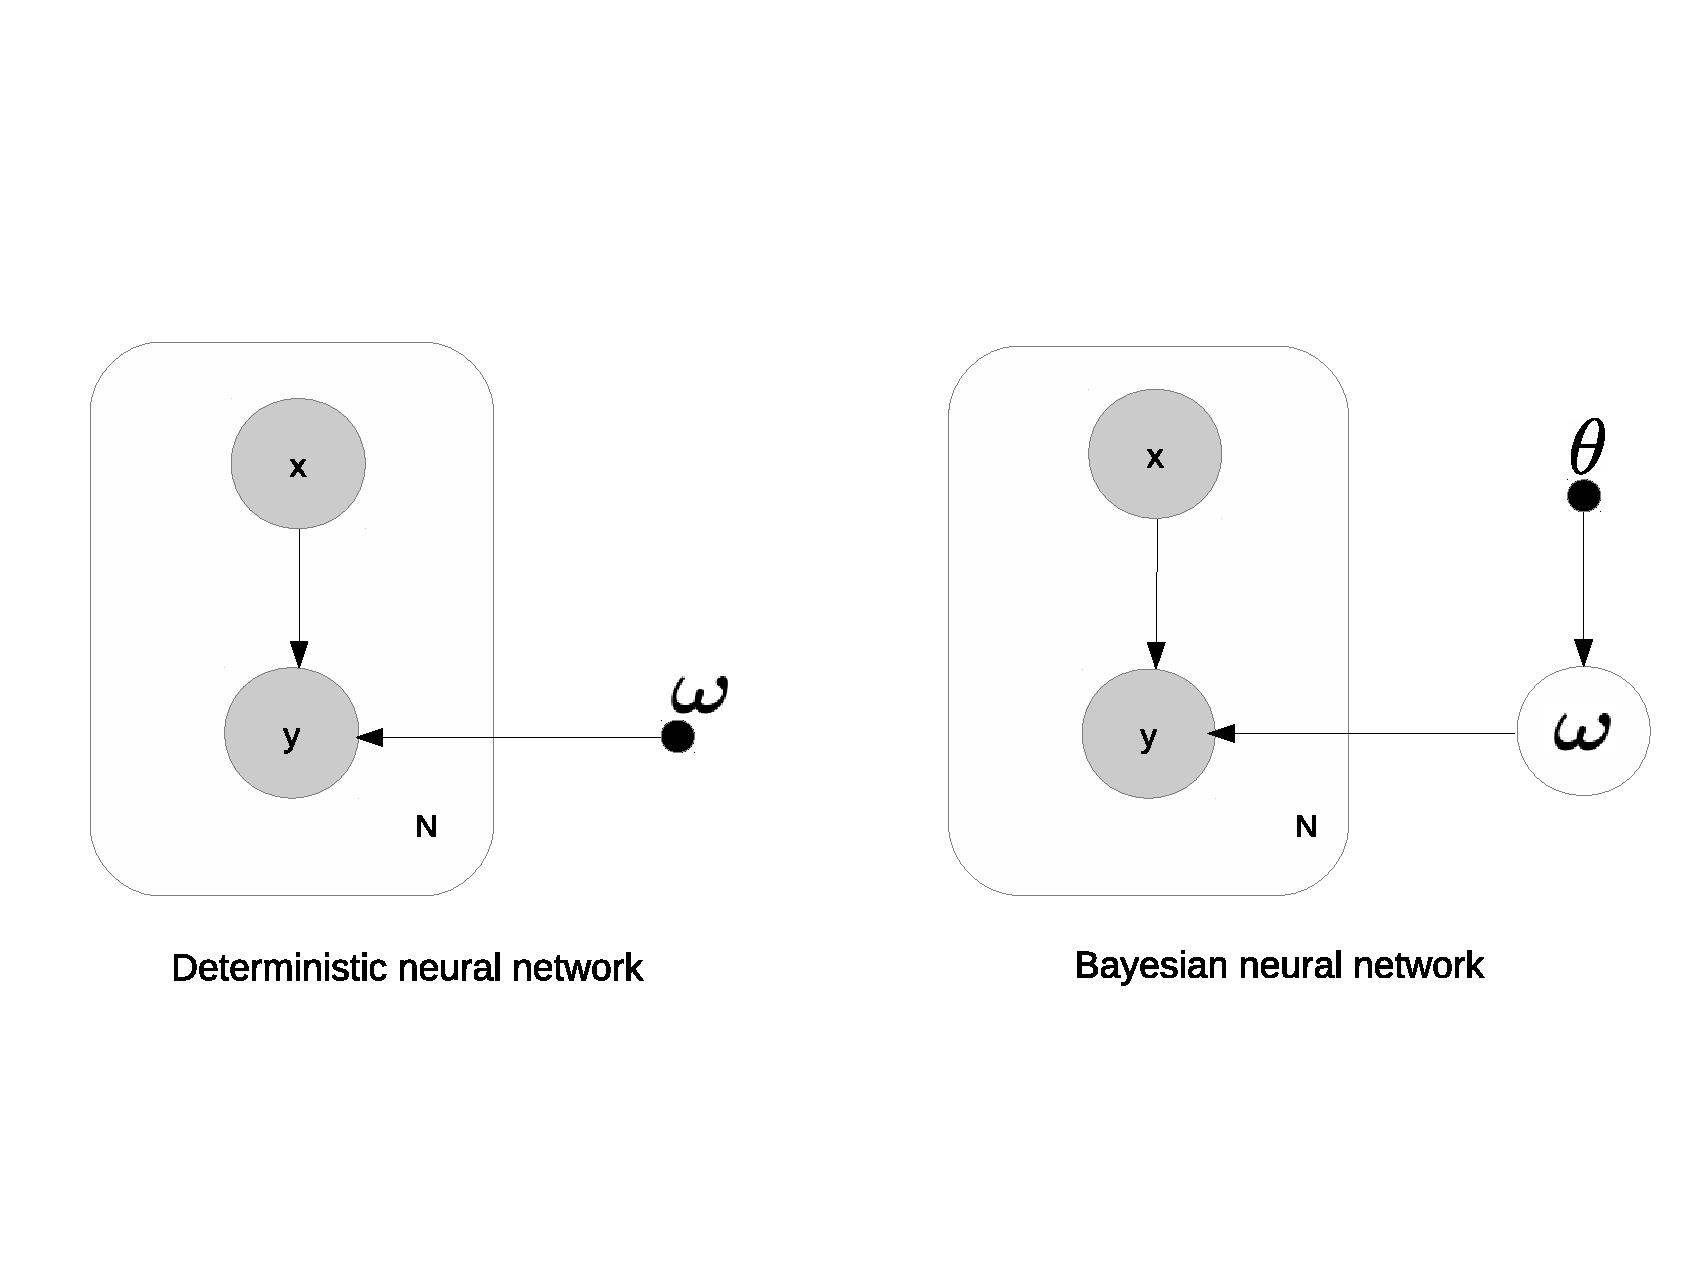
\includegraphics[width=15cm]{dnn_bnn}
		\caption{Difference between parameter estimation of deterministic neural network and Bayesian neural network.}		
		\label{fig:dnn_bnn}
	\end{center}
\end{figure}

\section{Variational inference}
\subsection{Introduction}
As is mentioned above, variational inference cast inference into optimization by minimizing the Kullbach-Leibler divergence between approximate posterior distribution and the real posterior distribution. However, there is no analytical definition of this KL divergence between the real posterior distribution is unkown. We can derive a lower bound which is also called evidence lower bound($ELBO$) which bounds the log marginal likelihood with Jensen's inequality. And from that we know marginal likelihood is the sum of $ELBO$ and KL divergence between approximate posterior and real posterior. The derivation is given in the following:
\begin{equation}\label{2.6}	
\begin{aligned}
	\log(p(\bld{Y}|\bld{X})) & = \log(\int p(\bld{Y}| \bld{X}, \bld{\omega})  p(\bld{\omega})d\bld{\omega}) \\	 
	& = \log(\int{q_{\theta}(\bld{\omega}) \frac{p(\bld{Y}| \boldsymbol{X}, \bld{\omega}) p(\bld{\omega})}{q_{\theta}(\bld{\omega})}d\bld{\omega}}) \\
	& \geq \int q_{\theta}(\bld{\omega}) \log( \frac{p(\bld{Y}| \bld{X}, \bld{\omega}) p(\bld{\omega})}{q_{\theta}(\bld{\omega})}) d\bld{\omega} \\
	& = \mathbb E_{q_{\theta}(\bld{\omega})}[\log(p(\bld{Y}| \bld{X}, \bld{\omega}))] -  KL(q_{\theta}(\bld{\omega}||p(\bld{\omega})))\\
	& = ELBO
\end{aligned}
\end{equation}

where $p(\bld Y| \bld X)$ is the likelihood, $p(\bld \omega)$ is the prior distribution over model parameters, $q_{\theta}(\bld \omega)$ is the approximate posterior distribution over parameters which is parameterized by $\theta$.

We can get log$(p(\bld Y) | \bld X)$ by adding $ELBO$ and KL divergence between approximate posterior $q_{\theta}(\bld \omega)$ and real posterior $p(\bld \omega | \bld X, \bld Y)$:

\begin{equation}\label{2.7}	
\begin{aligned}
 & ELBO + KL(q_{\theta}(\bld{\omega}) || p(\bld{\omega}|\bld{X}, \bld{Y})) \\ 
 & = \int q_{\theta}(\bld{\omega}) \log( \frac{p(\bld{Y}| \boldsymbol{X}, \bld{\omega}) p(\bld{\omega})}{q_{\theta}(\bld{\omega})}) d\bld{\omega} + \int q_{\theta}(\bld{\omega}) \log(\frac{q_{\theta}(\bld{\omega})}{p(\bld{\omega}|\bld{X}, \bld{Y})}) d\bld{\omega} \\
 & = \int q_{\theta}(\bld{\omega}) \log(p(\bld{Y} | \bld{X}))d\bld{\omega}\\
 & = log(p(\bld{Y}|\bld{X})) 
\end{aligned}
\end{equation}

When we maximize the $ELBO$ w.r.t the parameters of approximate posterior $\theta$, it's equivalent to minimizing the KL divergence because the log marginal likelihood is not a function of $\theta$. Then we have a well-defined objective which is the $ELBO$, in which the first term is called expected log likelihood which ensures the model can explain the data well and the second term is called regularization term which ensures the approximate posterior does not deviate too far from the prior distribution.
Now we have cast an inference problem into an optimization problem:

\begin{equation}\label{2.8}	
\begin{aligned}
\theta^{\star} = argmin_{\theta} [KL(q_{\theta}(\bld \omega)||p(\bld \omega | \bld X, \bld Y))]
\end{aligned}
\end{equation}

which is equivalent to 

\begin{equation}\label{2.9}	
\begin{aligned}
\theta^{\star} = argmax_{\theta} [ELBO]
\end{aligned}
\end{equation}

However, there are still some difficulties if we want to solve this optimization with this objective. The first one is to deal with large size dataset, which induces large computation in the expected log likelihood term. \cite{graves2011practical} shows that this can solved by data subsampling which is also called stochastic optimization. Another one is that we need to obtain the derivatives of $ELBO$ w.r.t. approximate parameter $\theta$. Since the model parameters are samples from approximate distribution, good estimator for the derivatives is required which will be introduced in next subsection. 


\subsection{Dropout variational inference}
\subsubsection{Dropout}
Dropout\cite{srivastava2014dropout} is originally introduced as regularization approach in training deep neural network which can improve the generalization performance. Although the author said this idea is inspired from human beings sexual reproduction, there are different interpretations trying to explain why it can work such as ensemble perspective and Bayesian perspective. In this subsection, the Bayesian interpretation of dropout is introduced and used for improving the uncertainty estimation of neural network. 

The mechanism of dropout is simple, each units of specific layer is multiplied by a random variable under Bernoulli distribution with $1-p$ as its parameter, where $p$ is dropout rate. In each iteration of training, dropout is turned on, which means each unit is multiplied by the sample drawn from Bernoulli distribution in forward propagation which is kept in  derivatives back propagtion during current iteration. In testing, the sampling phase is turned off, only one forward propagation is needed to obtain predictions. Normally, in order to avoid rescaling weights in testing, which is used to keep the output magnitudes in the same scale when dropout is off, rescaling of the output of dropout is always done in training. In figure \ref{fig:dropout}, there are two figures about that dropout is on and off. 
\begin{figure}[h!]
	\begin{center}
		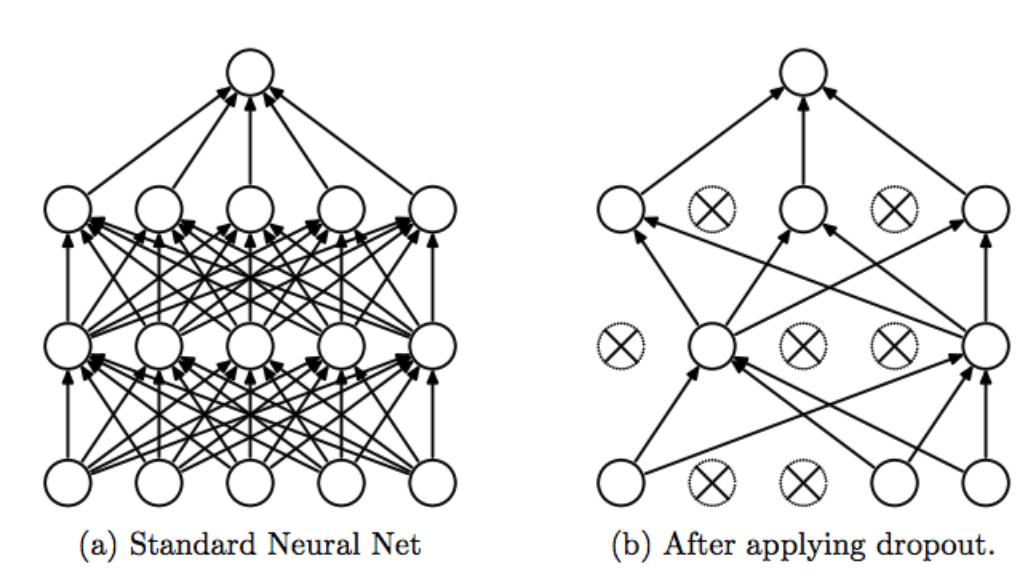
\includegraphics[width=13cm]{dropout}
		\caption{How dropout works\cite{srivastava2014dropout}.}		
		\label{fig:dropout}
	\end{center}
\end{figure}


\subsubsection{Bayesian interpretation of dropout}
As is mentioned in the last subsection, in variational inference, we want to minimize the KL divergence between approximate distribution and the real posterior distribution over the model parameters, which turns out to be maximization of evidence lower bound($ELBO$). When dropout is interpreted in Bayesian way, the distribution over hidden units is reformulated as distribution over weight matrices. The training objectives of neural network with dropout is proved to be similar as the $ELBO$ of Bayesian neural network with Bernoulli distribution factorized over the input dimension of weight matrix. In the following, we will explain this interpretation including key factors such as \textbf{approximate distribution}, \textbf{training objective}, \textbf{marginalization in testing} by using one simple example in {classification} case in \ref{fig:dropout_inference}, in which we define the hidden layer as the first layer and output layer as the second layer and assume that we use L2 regularization and put a prior distribution of fully factorized Gaussian over weights initially, which can be generalized to multi-layer neural network easily.


\begin{figure}[h!]
	\begin{center}
		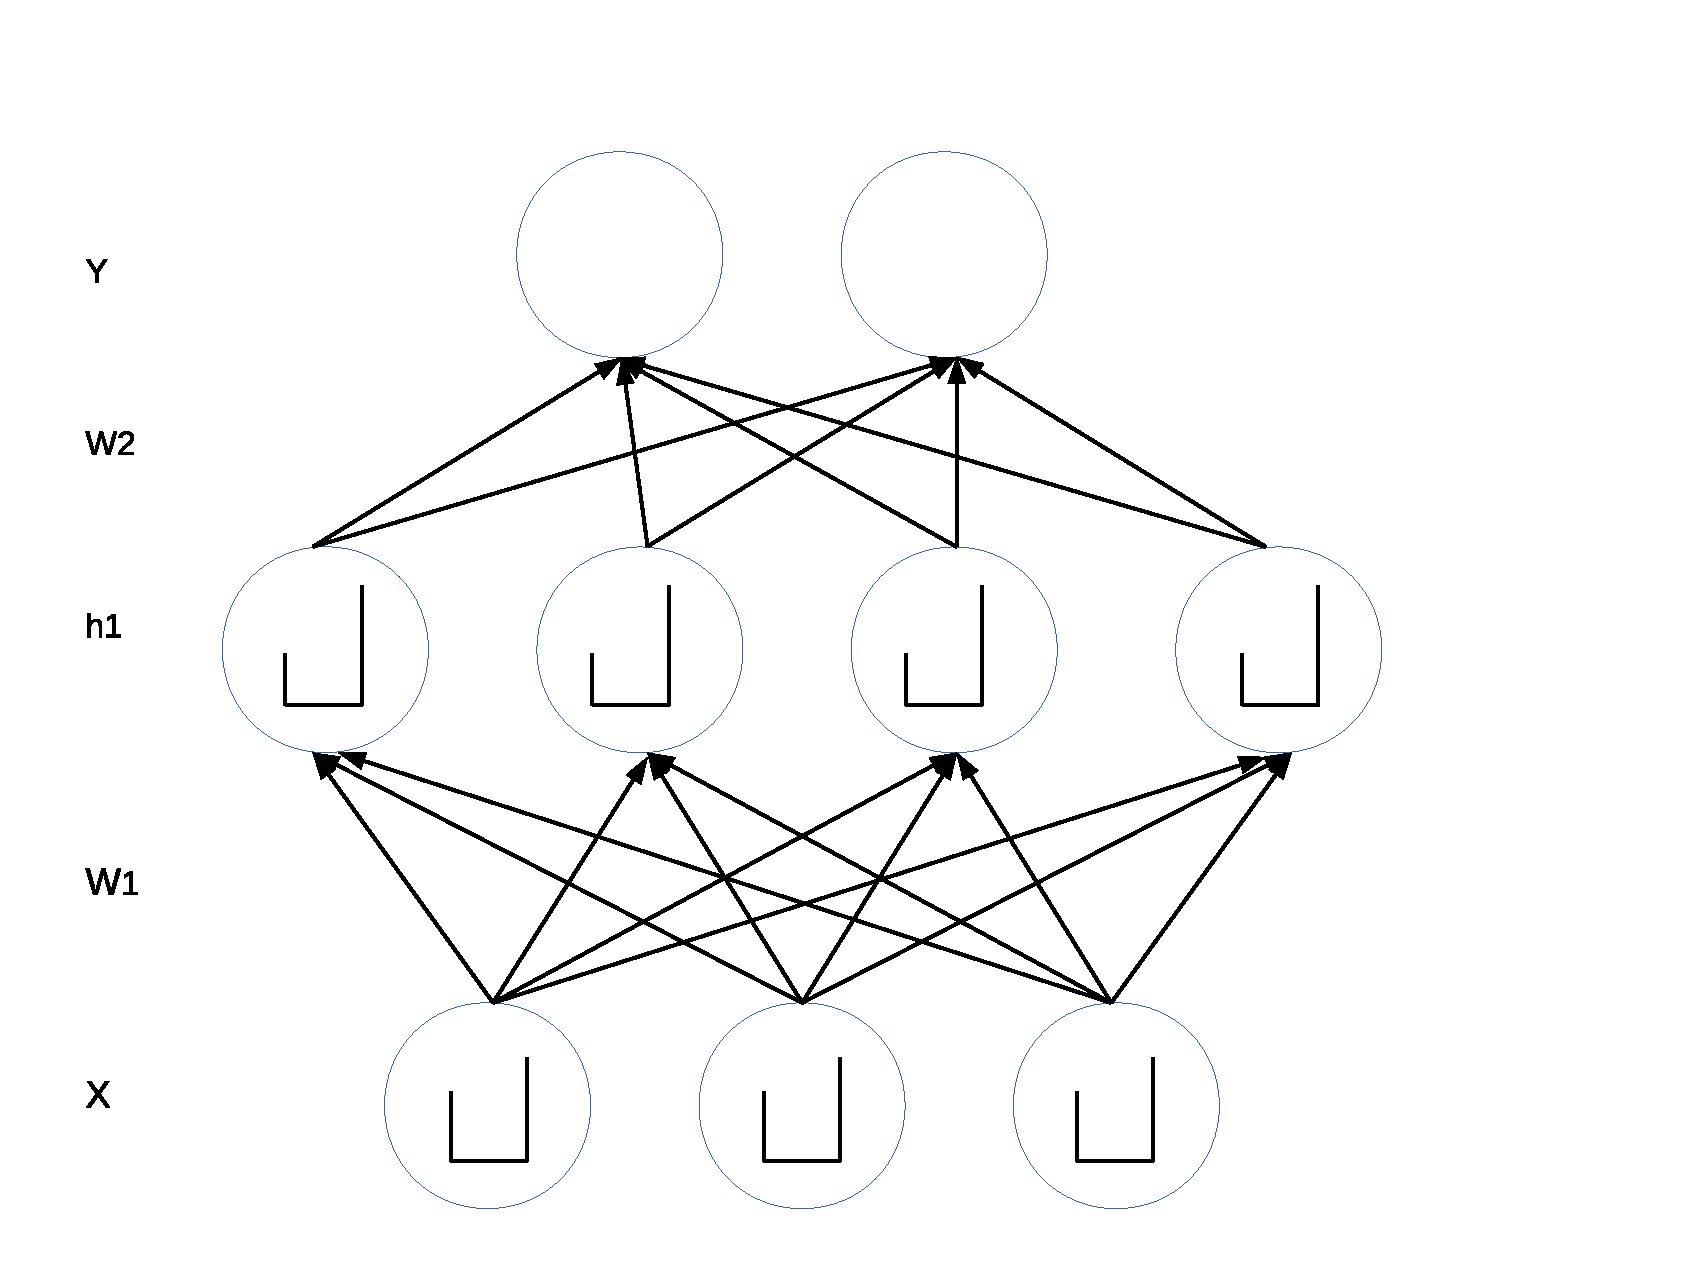
\includegraphics[width=10cm]{dropout_inference}
		\caption{A two layer neural network example of dropout inference, a Bernoulli random variable is imposed on each unit of input layer and hidden layer.}		
		\label{fig:dropout_inference}
	\end{center}
\end{figure}

\newpage
\paragraph{Approximate distribution}
Let's denote $\bld y\in \mathbb R ^{m \times D_{2}}$ as output, $\bld x \in \mathbb R^{m \times D_{0}}$ as input, $\bld h_{1} \in \mathbb R^{D_{1}}$ as the response of hidden layer, where $m$ represents number of data instances, $D_{i}$ is dimensionality of $i$-th layer, where $0$-th layer represents input layer and $i \in \{1,..,L\}$, $L=2$ in this example. Further we define $\bld \omega = \{ (\bld W_{i})_{i=1}^{L}  \}$ as model parameters, and $\bld \epsilon_{i} \in \mathbb R^{D_{i-1}}$ as the Bernoulli distributed random vector parameterized by $\bld p_{i} \in \mathbb R^{D_{i-1}}$, for $i$-th layer. In normal dropout, elements in vector $\bld p_{i}$ have same values $p_{i}$, which means that there is one keep rate or ($1-$dropout rate) for each layer. In the following, we will use $\bld p_{i}$ and $p_{i}$ interchangeably depending on the context if there is no special specification. To note that since weight matrix is treated as random variable, we use $\bld M_{i} \in \mathbb R^{D_{i-1} \times D_{i}}$ to denote position of non-zero element in Bernoulli distribution for $\bld W_{i}$. To note that bias $\bld b_{i} \in \mathbb R^{D_{i}}$ is absorbed into $W_{i}$ by appending a new row at the end of weight matrix and 1 at the end of each data input vector, which is also called homogeneous coordinate. We also assume that approximate weight distribution is factorized over layer, which yields
\[
q_{\theta}(\bld \omega) = \prod_{i=1}^{L}q_{\theta}(\bld W_{i}). 
\]

To start with the formulation of dropout, we model likelihood of output conditioned on input with softmax scores of neural network in classification case:
\begin{equation}
	\begin{aligned} \label{dropout_form}
	p(\bld y| \bld x, \bld \omega) & = \sigma((\bld h_{1} \odot \bld \epsilon_{2}) \bld M_{2})\\
		   & = \sigma(\bld h_{1} (diag(\bld \epsilon_{2}) \bld M_{2})) \\
		   & = \sigma(\bld h_{1} \bld W_{2}) \\
		   & = \sigma(a(\bld x (diag(\bld \epsilon_{1}) \bld M_{1})+ \bld b_{1}) \bld W_{2}) \\
		   & = \sigma(a(\bld x \bld W_{1})\bld W_{2})
	\end{aligned}
\end{equation}

where $\odot$ is Hadamard product(element-wise product), $\sigma(a_{j}) = \frac{exp({a_{j}})}{\sum_{k}exp({a^{k}})}$ is softmax function, $a(\cdot)$ is non-linear activation function such as rectified unit function.
  
From the equation above, we have 

\[
\bld W_{i} = g(\bld M_{i}, \bld \epsilon_{i})= diag(\bld \epsilon_{i}) \bld M_{i} 
\]
\[ 
\text{ with } \bld \epsilon_{i} \sim p(\bld \epsilon_{i}) = Bernoulli(\bld p_{i}) 
\]

which means weight matrix $\bld W_{i}$ is a random variable whose probability density function is parameterized by $\bld p_{i}$ and $\bld M_{i}$, which are denoted by $\theta = \{ (\bld M_{i}, \bld p_{i})_{i=1}^{L} \}$ in equation \ref{2.8}, where $i = {1,..,L}$ denotes $i$-th layer of the network, and $L = 2$ in this example. 
The expression of approximate posterior distribution is not obvious, but we can define the its form as 

\begin{equation}
\begin{aligned} \label{appro_dist_form}
q_{\theta}(\bld \omega) &= \prod_{i=1}^{L} q_{\theta}(\bld W_{i})\\
&= \prod_{i=1}^{L}\int q_{\theta}(\bld W_{i} | \bld \epsilon_{i})p(\bld \epsilon_{i}) d\bld \epsilon_{i} 
\end{aligned}
\end{equation}
with

\begin{equation}
\begin{aligned} \label{appro_cond_dist_form}
q_{\theta}(\bld W_{i}|\bld \epsilon) &= \delta(\bld W_{i} - g(\bld M_{i}, \bld \epsilon_{i}))  \\
& = \delta(\bld W_{i} - diag(\bld \epsilon_{i})\bld M_{i})
\end{aligned}
\end{equation}

As we can see, the approximate posterior distribution over the parameter matrix puts a same Bernoulli distribution over the input dimension of parameter matrix, which is the row dimension in this example.  Meanwhile each element of the same row is multiplied with same realization of the random variable but with different non-zero position, which is corresponding to different expectation of each row element and thus induces correlations between row elements. To make this definition more clear, based on the computation of expectation and variance of Bernoulli distribution, we can write down the first and second moment of the approximate distributed random variables in the following:

\begin{equation}
\begin{aligned} \label{appr_expectation}
\mathbb E_{q_{\theta}}(\bld W_{i}) & = \bld M_{i} \odot \bld P_{i}
\end{aligned}
\end{equation}

where $\bld P_{i} = [\bld p_{i}, ..., \bld p_{i}] \in \mathbb R^{D_{i-1} \times D_{i}}$.

Covariance matrix of parameter matrix is:

\begin{equation}
\begin{aligned} \label{appr_covariance}
 \big[Cov_{q_{\theta}}(vec(\bld W_{i}))\big]_{jk}   = \mathbbm{1} \big[l=m\big] m^{i}_{lq}*m^{i}_{mn}*p_{i}*(1-p_{i})
\end{aligned}
\end{equation}

where 
\[ j = l*D_{i-1} + q\],
\[ k = m*D_{i-1} + n\],
which is the linear mapping between element index before and after matrix vectorization. $m^{i}_{lq}$ is the element of $l$-th row and $q$-th column in matrix $\bld M_{i}$, which applies to $m^{i}_{mn}$ as well. $\mathbbm 1 \big[i=j\big]$ denotes indicator function, which is equal to 1 only when $i$ is equal to $j$ and otherwise 0. Because $vec(\cdot)$ operation converts matrix $\bld W_{i} \in \mathbb R^{D_{i-1} \times D_{i}}$ into column vector $ vec(\bld W_{i}) \in \mathbb R^{D_{i-1}D_{i} \times 1}$ by stacking the columns of matrix on top of one another. Then it's easy to see that covariance matrix $Cov_{q_{\theta}}(vec(\bld W_{i})) \in \mathbb R^{D_{i-1}D_{i} \times D_{i-1}D_{i}} $. 

From equation \ref{appr_covariance}, we can see that the entire covariance matrix is consisting of $D_{i} \ast D_{i}$ diagonal sub-matrices whose dimensionality are $D_{i-1} \times D_{i-1}$.
When observing covariance matrix of parameter matrix $\bld W_{i}$ w.r.t. approximate posterior distribution $q_{\theta}({\bld W_{i}})$, we know that samples of row vectors in weight matrix are drawn independently and thus covariance between rows are zero. On the other hand, samples for different weights in the same row are drawn at the same time because they are multiplied by the same realization of $\epsilon_{i}$, from which covariances between weights within the same row are induced. Therefore, by fitting this approximate distribution to the real posterior distribution weights within the same row can be learned. This means that the approximate distribution family have more flexibility to approximate the real posterior distribution when compared with other common approximate posterior distribution family that assumes distribution for each parameter is independent such as fully factorized Gaussian.


\paragraph{Training objective} Up to now, we have only analyzed the approximate distribution of dropout inference. As is mentioned in introduction section of this chapter, we know that we perform optimization of $ELBO$ w.r.t. the approximate distribution parameters, in order to obtain a good approximation to the true posterior distribution over parameters, which we can use in testing to obtain more reliable uncertainty estimation. In the following, we will show that training a neural network with dropout is equivalent to optimizing the $ELBO$ w.r.t. approximate distribution parameters.

At first, let's define the training objective of neural network with dropout, which is cross entropy between predictive distribution and target distribution plus L2 regularization:

\begin{equation}
\begin{aligned} \label{dropout_loss}
L_{dropout}   = \sum_{i=1}^{N}\big[-log(p(\bld y_{i}| \bld x_{i}, \bld \omega))\big] + \lambda(\sum_{i=1}^{L} ||\bld W_{i}||^{2})
\end{aligned}
\end{equation}

where $N$ represents the size of entire dataset, $\lambda$ is L2 regularization coefficient. We want to maximize the likelihood over the entire dataset w.r.t. the model parameter $\bld \omega$, which is known as maximum likelihood estimation. Equipped with L2 regularization and Gaussian prior over parameters, we can obtain a max-a-posterior estimation by minimizing equation \ref{dropout_loss}. 

Normally we use gradient descent to tune our parameters in training, which requires first derivative of objective w.r.t. model parameters $\bld \omega$. Since nowadays large size of dataset is ubiquitous, which means $N$ in equation \ref{dropout_loss} is too large, we could not obtain exact gradient of entire batch with efficient computation. Therefore we use data of mini-batch to estimate gradient, which is so called stochastic gradient descent(SGD). Apart from making computation tractable, noise of gradient estimation in each mini-batch is helpful for optimization procedure to escape the poor local minimum. The expression of gradients required in each iteration of SGD is given in the following:

\begin{equation}
\begin{aligned} \label{dropout_grad}
\frac{\partial L_{dropout}}{\partial \bld \omega} &=\frac{1}{K}\sum_{i \in S}\big[-\frac{\partial log(p(\bld y_{i}| \bld x_{i}, \bld \omega))}{\partial \bld \omega}\big] + \lambda\frac{\partial (\sum_{i=1}^{L} ||\bld W_{i}||^{2})}{\partial \bld \omega}
\end{aligned}
\end{equation}

where $S$ is one random subset of entire dataset, and $|S| = K$.

On the other hand, let's have a look at $ELBO$ in equation \ref{2.6}, if we want to maximize $ELBO$, which is equivalent to minimize negative $ELBO$ w.r.t. the approximate distribution parameters $\theta$, with SGD. The gradients are computed with the following expression:

\begin{equation}
\begin{aligned} \label{elbo_grad}
\frac{\partial (-ELBO)}{\partial \theta} &=\frac{1}{K}\sum_{i \in S}\big[-\frac{\partial \mathbb E_{q_{\theta}(\bld \omega)} \big[log(p(\bld y_{i}| \bld x_{i}, \bld \omega))\big]}{\partial \theta}\big] + \frac{\partial KL(q_{\theta}(\bld \omega)||p(\bld \omega))}{\partial \theta}
\end{aligned}
\end{equation}

In order to calculate two terms in equation \ref{elbo_grad}, we need to introduce one technique called re-parameterization trick\cite{kingma2013auto} for the first term and one condition called KL condition\cite{gal2016uncertainty} for the second term in the following.

\subparagraph{Re-parameterization trick:} when we take a close look at the first term in equation \ref{elbo_grad}, we know that we need to compute the gradients of expectation w.r.t. the parameters of distribution to which this expectation is subject. That means, we need to estimate the gradients of those parameters because our objective is generated from these parameters randomly. Fortunately, there are different approaches to estimate the gradients of this kind of parameters such as score function or REINFORCE estimator\cite{williams1992simple}, re-parameterization trick \cite{kingma2013auto} and so on. As is stated in \cite{kingma2013auto}, re-parameterization trick has lower variance than score function estimator and is also unbiased. Let's have a quick recap of this technique and see it's already a built-in part in neural network with dropout.

To identify the problem, we can write a more general form of calculus we want to solve in the following:

\begin{equation}
\begin{aligned} \label{repa}
I(\theta) = \frac{\partial}{\partial \theta} \mathbb E_{p_{\theta}(x)} \big[ f(x)\big]= \frac{\partial}{\partial \theta} \int f(x) p_{\theta}(x) dx
\end{aligned}
\end{equation} 

Assume that $p_{\theta}(x)$ can be re-parameterized as $p(\epsilon)$ which is a parameter-free distribution such that random variable $x$ can be generated from a deterministic differentiable function with $\theta$ and $\epsilon$ as arguments, that is

\[
x = g(\theta, \epsilon)  \text{ with } \epsilon \sim p(\epsilon)
\]

Then we can derive the estimator of the gradients w.r.t. distribution parameters $\theta$ with $p(x|\epsilon) = \delta(x-g(\theta,\epsilon))$:
\begin{equation}
\begin{aligned} \label{repa1}
I'(\theta) &= \frac{\partial}{\partial \theta} \int f(x) p_{\theta}(x) dx \\
&= \frac{\partial}{\partial \theta} \int f(x)(\int p_{\theta}(x|\epsilon)p(\epsilon)d\epsilon) dx \\
&= \frac{\partial}{\partial \theta} \int (\int f(x) p_{\theta}(x|\epsilon)dx) p(\epsilon) d\epsilon \\
&= \frac{\partial}{\partial \theta} \int (\int f(x)\delta(x-g(\theta,\epsilon))dx) p(\epsilon) d\epsilon \\ 
&= \frac{\partial}{\partial \theta} \int f(g(\epsilon, \theta)) p(\epsilon) d\epsilon \\
&= \int \frac{\partial}{\partial \theta} f(g(\epsilon, \theta)) p(\epsilon) d\epsilon \\
&= \int f'(g(\epsilon, \theta))\frac{\partial}{\partial \theta}g(\theta, \epsilon) p(\epsilon) d\epsilon \\
&= \mathbb E_{p(\epsilon)}\big[ f'(g(\epsilon, \theta))\frac{\partial}{\partial \theta}g(\theta, \epsilon)\big] 
\end{aligned}
\end{equation} 
From practical point of view, the expectation of last line in expression \ref{repa1} can be approximated with Monte Carlo integration. In dropout inference, we know that if we fix the dropout rate which is equal to $1- p_{i}$ in equation \ref{appro_cond_dist_form} in training. Then $\bld \epsilon_{i}$ in equation \ref{appro_cond_dist_form} is a parameter free random variable and $g(\cdot)$ is a differentiable function w.r.t. parameter $\bld M_{i}$. And the approximate distribution parameter $\theta$ only contains $\{(\bld M_{i})_{i=1}^{L} \}$, which are exactly the weights to be learned in training neural network with dropout. As a result, if we estimate the gradient of $ELBO$ w.r.t. approximate distribution parameters $\{(\bld M_{i})_{i=1}^{L}\}$, that is the first term in \ref{elbo_grad}, it's equivalent to calculate the gradient of dropout loss w.r.t. model parameters $\bld \omega$ which is the first term in equation \ref{dropout_grad}.

\subparagraph{KL condition:} The second term in equation \ref{elbo_grad} is proved to be equivalent to the second term in equation \ref{dropout_grad}
for a large enough number of hidden units when we specify the model prior to be a product of independent Gaussian distributions over each weight with prior length scale $l$, that is:
\[p(\bld \omega) = \prod_{i=1}^{L}(p(\bld W_{i})) \]
with
\[
p(vec(\bld W_{i})) = \mathcal N(0, l^{-2}\bld I_{D_{i-1} D_{i}})
\]

To establish this condition, we need to make a approximation of the approximate posterior distribution $q_{\theta}(\bld \omega)$ in equation \ref{appro_dist_form}, where we approximate $q_{\theta}(\bld W_{i}|\bld \epsilon_{i})$ in equation \ref{appro_cond_dist_form} as a narrow Gaussian with a very small standard deviation. As we know, $q_{\theta}(\bld W_{i})$ factorizes over each row of the weight matrix. Then that means $q_{\theta}(\bld \omega)$ is a mixture of two Gaussians with small standard deviations, and one component fixed at zero:
\begin{equation}\label{appro_dist_guassian}
\begin{aligned}
	q_{\theta}(\bld \omega) &= \prod_{i=1}^{L}q_{\theta}(\bld W_{i}) \\
	&=\prod_{i=1}^{L}\prod_{j=1}^{D_{i-1}}q_{\theta}(\textbf{w}_{i,j}) \\
	&= \prod_{i=1}^{L}\prod_{j=1}^{D_{i-1}} \big[ p_{i} \mathcal N(\textbf{m}_{i,j},\sigma^{2} \bld I_{D_{i}}) + (1-p_{i})\mathcal N(\bld 0, \sigma^{2} \bld I_{D_{i}})\big]
\end{aligned}
\end{equation}
where $\textbf{w}_{i,j} \in \mathbb R^{D_{i}}$ is the $j$-th row of weight matrix $\bld W_{i}$ and $p_{i}$ is the parameter of Bernoulli distributed random variable of $i$-th layer. With this, the KL divergence between approximate posterior and prior is KL divergence between mixture of Gaussian and a single Gaussian. In order to keep this report as self-contained as possible, we attach the derivation of KL divergence between mixture of Gaussian and single Gaussian in appendix \ref{appendix:kl_condition}. Then we have KL condition in the following:

\begin{equation}
\begin{aligned} \label{kl_condition}
KL(q_{\theta}(\bld \omega) || p(\bld \omega)) \approx \sum_{i=1}^{L} \sum_{j=1}^{D_{i-1}}
\big[
\frac{p_{i}}{2}(l^{2}\bld m_{i,j}^{T} \bld m_{i,j} + D_{i}( \sigma^{2} -\text{log}(\sigma^{2}) -2\text{log} l- 1) - \mathcal H (\bld p_{i}) 
\big] 
\end{aligned} 
\end{equation}
with 
\[
\mathcal H(\bld p_{i}) = D_{i-1}(-p_{i}\text{log}p_{i} - (1-p_{i})\text{log}(1-p_{i}))
\]
for large enough $D_{i}$. If we fix dropout rate in training and compute the gradients of KL divergence w.r.t. model parameters $\theta = \{(\bld M_{i})_{i=1}^{L} \}$. We can see that, if we choose $\lambda = \frac{l^{2}p_{i}}{2}$, then it's equivalent to the gradients of regularization term in dropout loss function(cf. \ref{dropout_grad}):

\begin{equation} 
\begin{aligned}\label{KL_grad}
\frac{\partial KL(q_{\theta}(\bld \omega)||p(\bld \omega))}{\partial \theta} \approx \frac{\partial \sum_{i=1}^{L}\lambda||\bld M_{i}||^{2}}{\partial \theta}
\end{aligned}
\end{equation}

With aforementioned re-parameterization trick and KL condition, we know that the computation of gradients of objective function w.r.t. model parameters in equation \ref{dropout_grad} is equivalent to those of $ELBO$ w.r.t. approximate distribution parameters in equation \ref{elbo_grad}. That means if we train a neural network with dropout, we can obtain the approximate posterior distribution over model parameters defined in equation \ref{appro_dist_form}.

\paragraph{Marginalization in testing}
After we have obtain the parameters $\theta$ of approximate posterior distribution over model parameters $q_{\theta}(\bld \omega)$, we can marginalize all possible parameters over approximate posterior to get final predictive distribution of output, similar to equation \ref{2.4} but with approximate posterior. Because the integration is hard to evaluate analytically. In practice, we always use Monte Carlo integration:

\begin{equation}
\begin{aligned} \label{marginalization_test}
p(\bld y^{\star}| \bld x^{\star},\mathcal D) &= \int p(\bld y^{\star} | \bld x^{\star}, \bld \omega) p(\bld \omega |\mathcal D)d\bld \omega \\
&\approx \int p(\bld y^{\star} | \bld x^{\star}, \bld \omega) q_{\theta}(\bld \omega)d\bld \omega \\
&\approx \frac{1}{K}\sum_{i=1}^{K} p(\bld y^{\star} | \bld x^{\star}, \bld{\hat \omega_{i}}) 
\end{aligned}
\end{equation}

where $\bld \omega \sim q_{\theta}(\bld \omega)$ and $\bld{\hat \omega_{i}}$ is one of $K$ realizations of $\bld \omega$, which is equivalent to turning on dropout in testing time. This is also called \textbf{MC-dropout} in the literatures.

\subsection{Concrete dropout and Multi-Drop}
\paragraph{Concrete dropout} 
Based on the aforementioned description of dropout inference, we can see that if we fix dropout rate in training, then parameters of approximate distribution $\theta$ only contains $\{\bld M_{i}\}_{i=1,...,L}$, which is equivalent to $\bld \omega = \{\bld W_{i}\}_{i=1,...,L}$ in neural network with dropout. Therefore optimising any neural network with dropout is equivalent to a form of approximate inference in a probabilistic interpretation of the model. This means that the optimal weights found through the optimization of a neural network with dropout are the same as the optimal variational parameters in a Bayesian neural network with the same structure. 

However, fixing dropout rate in train is not a trivial task for several reasons. Firstly, as is shown in \cite{srivastava2014dropout}, different dropout rates have different impact on model capacity and thus model performance. To choose an optimal dropout rate manually requires repeating tedious experiments and thus waste of time and computation effort. Secondly, if we want our model not only to achieve satisfied performance but also to possess reliable uncertainty estimation, the dropout rate matters a lot because it belongs to variational parameter $\theta$ and further influences the flexibility of approximate distribution family from the perspective of Bayesian interpretation.

Accordingly, one direct counter measure is to learn dropout rate from the data \cite{gal2017concrete}. One major difficulty to learn dropout rate from the data in gradient-based optimization is that it's not trivial to estimate gradients of expectation w.r.t. parameters of the distribution when this distribution is discrete. Before in case of continuous distribution, we estimate this gradient with help of re-parameterization trick. As introduced in the last section, re-parameterization trick requires re-parameterizing model parameters by a differential function with variational parameters and a parameter-free random variable as input arguments. For continuous distribution, this function can be found easily if they have tractable inverse cumulative density function or functional form like Gaussian\cite{kingma2013auto}. For most of discrete distributions such as Bernoulli distribution or categorical distribution, they lack useful reparameterizations
due to the discontinuous nature of discrete states \cite{maddison2016concrete}. 

Faced with this issue, \cite{jang2016categorical} and \cite{maddison2016concrete} come up with one approach that replaces "max" operation in Gumbel-Max trick with softmax function, which can yields a practical re-parameterization for discrete random variable. With this method, gradients w.r.t. parameters of discrete distribution can be computed and used in gradient-based optimization. In this subsection, a quick recap of this method is given in the following.

\subparagraph{Re-parameterization of Bernoulli distribution}
Firstly, Gumbel-Max trick\cite{maddison2014sampling} is introduced in figure \ref{gumbel_max}, which is used for drawing samples from a discrete distribution which is parameterized by set of unnormalized probability $\{\alpha_i\}_{i=1}^{n}$ via inverse cumulative distribution function of Gumbel distribution, where $\alpha_i \in \mathbb R_{>0}$ and $n$ denotes the number of class. Assuming that we use one-hot encoding vector for the class representation, that is $\bld d \in \{0,1\}^n $ and $\sum_{i=1}^{n}d_i = 1$. The Gumbel-Max trick proceeds as follows(cf. figure \ref{gumbel_max}):
\begin{itemize}
	\item sample $G_i \sim \text{Gumbel}(0,1) = -\text{log}(-\text{log}(\text{Uniform}(0,1)))$, for $i=1,..,n$
	\item compute $x_i = $log($\alpha_i$) + $G_i$, for $i=1,..,n$
	\item set $d_k = 1$, where $k=argmax_i\{x_i\}_{i=1,..n}$, and $d_i = 0$ for $i \neq k$
\end{itemize}
Then we obtain one sample from this discrete distribution and the probability for specific class.

\begin{figure}[h!]
	\begin{center} \label{gumbel_max}
		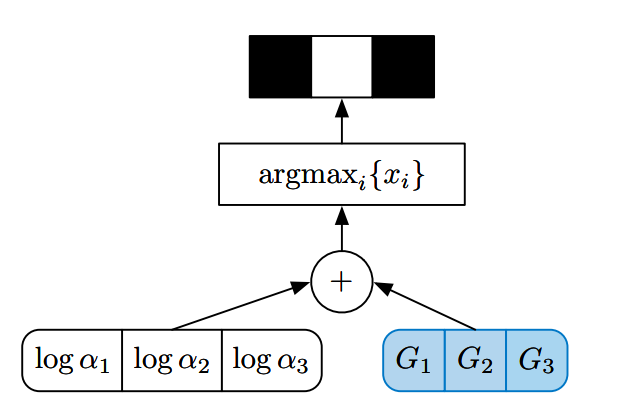
\includegraphics[width=9cm]{gumbel_max}
		\caption{Example of Gumbel-max trick for drawing samples from a discrete distribution whose random variable has 3 states and $\{\alpha_{i}\}_{i=1,2,3}$ as class parameters representing the possibility of occurrence of that class. $\{G_{i}\}_{i=1,2,3}$ are i.i.d Gumbel$(0,1)$ \cite{maddison2016concrete}.}		
		\label{fig:gumbel_max}
	\end{center}
\end{figure}

As observed in Gumbel-Max trick, the sampling step is re-paramterized by one function with distribution parameters and parameter-free random variable as arguments. This function is componentwise addition of two input arguments followed by $argmax$ operation. However, $argmax$ operation is not differential w.r.t. distribution parameter $\alpha_i$. Fortunately, this operation can be approximated by a continuous function, $softmax$, which is also differential w.r.t. distribution parameters. With this replacement, we can obtain a continuous approximation to $\bld d$ on the simplex $\triangle^{n-1} = \{\bld x \in \mathbb R^n | x_k \in [0,1], \sum_{i=1}^{n} x_i = 1 \}$:

\begin{equation} \label{gumbel_softmax}
\begin{aligned}
x_{k} = \frac{\text{exp}((\text{log}\alpha_k + G_k)/\lambda)}{\sum_{i=1}^{n}\text{exp}((\text{log}\alpha_i + G_k)/\lambda)}
\end{aligned}
\end{equation}

The sampling steps are similar to Gumbel-Max trick, but with smoothed $softmax$ operation instead of $argmax$(cf. figure \ref{fig:gumbel_softmax}). When $\lambda \rightarrow 0$, the $softmax$ function is recovered to $argmax$ operation, when $\lambda \rightarrow \infty$, this operation generates uniform vector instead of one-hot encoded vector.

\begin{figure}[h!]
	\begin{center}
		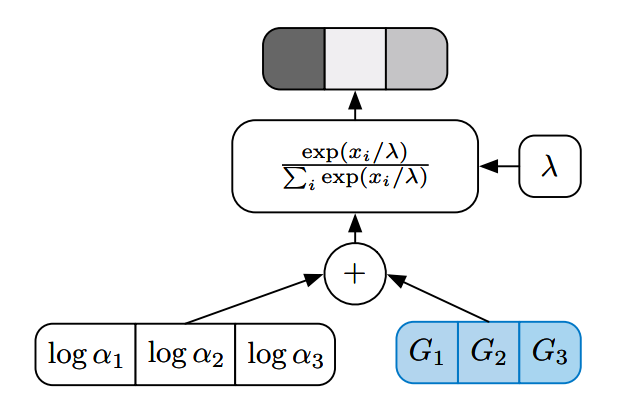
\includegraphics[width=9cm]{gumbel_softmax}
		\caption{Example of continuous approximation to Gumbel-max trick for drawing samples from a discrete distribution whose random variable has 3 states and $\{\alpha_{i}\}_{i=1,2,3}$ as class parameters representing the possibility of occurrence of that class. $\{G_{i}\}_{i=1,2,3}$ are i.i.d Gumbel$(0,1)$\cite{maddison2016concrete}.}		
		\label{fig:gumbel_softmax}
	\end{center}
\end{figure}

When it comes to Bernoulli discrete distribution in our case, it becomes similar because there are only two states in this distribution and samples live in two dimensional simplex. On the other hand, the difference of two Gumbels distributed random variable is similar to a logistic distributed random variable.  With the probability of state 1 which can be expressed by:

\[
\begin{aligned}
\mathbb P(d_1 = 1) &= \mathbb P(\text{log} \alpha_1 + G_1 >\text{log} \alpha_2 + G_2)\\
&=\mathbb P(\text{log} \alpha_1 - \text{log} \alpha_2 + G_1 - G_2 > 0)
\end{aligned}
\] 

where $G_1 - G_2 = \text{log}(\text{Uniform}(0,1)) - \text{log}(1-\text{Uniform}(0,1))$, which is the inverse cumulative density function of Logistic(0,1).
Then we can infer the re-parameterization of Bernoulli distributed variable with $p$ as parameter as follows:

\begin{equation}\label{bern_repa}
	\begin{aligned}
	x_1 = \text{sigmoid}\big(
	\frac{1}{\lambda} (\text{log}p - \text{log}(1-p) + \text{u} - \text{log}(1-u)) 
	\big)
	\end{aligned}
\end{equation}

where $u \sim \text{Uniform}(0,1)$. 

In order to make explanation more clear and validate this re-parameterization, there is one plot in the following (figure \ref{fig:bern_repa}) showing the relationship between average values of 100 samples drawn from this continuous approximation of Bernoulli distribution with different probability. We can see that the samples drawn from equation \ref{bern_repa} distributed similar to the Bernoulli distribution, while most of samples lie on the boundary of range $[0,1]$ and only few of them lie in the interior.
\begin{figure}[h!]
	\begin{center}
		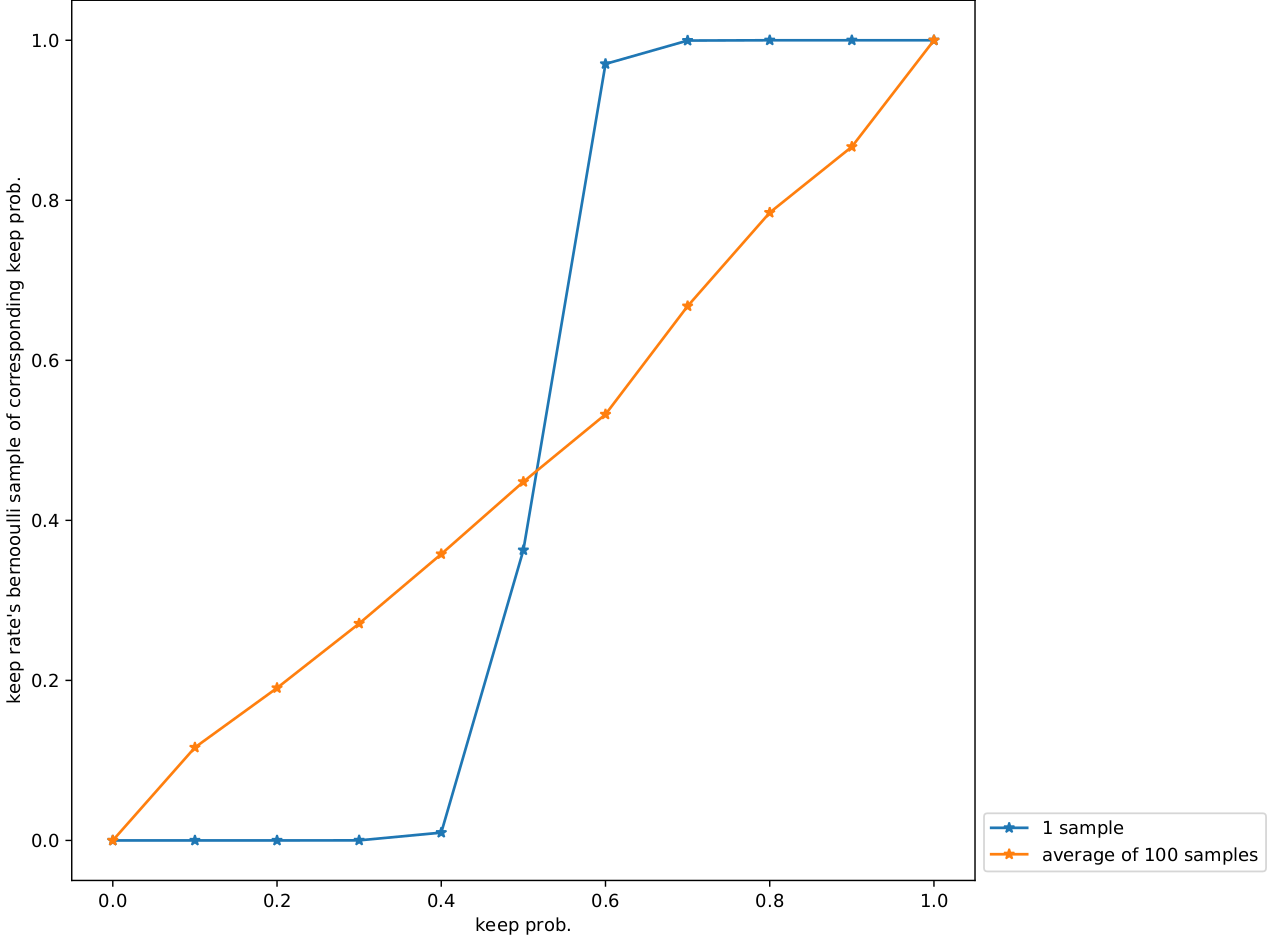
\includegraphics[height=7cm, width=13cm]{bern_repa}
		\caption{One sample and average value of 100 samples drawn from continuous approximation of Bernoulli distribution with parameter $p = [0.1, 0.2, ..., 1.0]$ and temperature $ \lambda =0.1$.}		
		\label{fig:bern_repa}
	\end{center}
\end{figure}

\subparagraph{Dropout regularization}
Because keep rate of dropout is optimized now, the parameters of approximate distribution $\theta$ contains both $\{ (\bld M_i)_{i=1}^{L} \}$ and $\{(\bld p_i)_{i=1}^{L} \}$. In order to compute gradients of ELBO in equation \ref{elbo_grad}, we employ categorical re-parameterization to estimate the gradients w.r.t. Bernoulli distribution parameter $\bld p_i$ in the first term, for the second term, we could not ignore the term with $\bld p_i$ in KL condition \ref{kl_condition}, which is the entropy term. Consequently, unlike equation \ref{KL_grad}, the KL divergence term should be:

\begin{equation} 
\begin{aligned}\label{KL_grad_concrete}
\frac{\partial KL(q_{\theta}(\bld \omega)||p(\bld \omega))}{\partial \theta} 
&\approx \frac{\partial \sum_{i=1}^{L}\lambda||\bld M_{i}||^{2}- \mathcal H(\bld p_{i})}{\partial \theta}  \\
&= \frac{\partial}{\partial \theta} \big( \sum_{i=1}^{L}\lambda||\bld M_{i}||^{2}- D_{i-1}(-p_{i}\text{log}p_{i} - (1-p_{i})\text{log}(1-p_{i}))\big)
\end{aligned}
\end{equation}

From the equation above, we can see that this term maximize the entropy of Bernoulli distribution, which means this term pushes $\bld p_i$ to 0.5. The coefficient of the dropout regularisation term means that large models will push the dropout probability towards 0.5 much more than smaller models, but as the amount of data N increases the dropout probability will be pushed towards 1 because of the expected log likelihood in the first term. One of reasons behind could be pushing $\bld p_i$ to 0.5 would decrease the capacity of the model which will decrease the expected log-likelihood. 

\paragraph{Multi-Drop}
From figure \ref{fig:dropout} and expression of approximate distribution in equation \ref{appro_dist_form}, we choose one probability of Bernoulli distributed random variable for each layer, therefore random vector $\bld p_i = [p_i]^{D_{i-1}}$. While the dropout regularization term push the probability of Bernoulli to 0.5, the expected likelihood term tries to increase the probability. An equilibrium state between them should be achieved in training. With concrete dropout introduced above, we could extend dropout for each hidden units instead of each layer(cf. figure \ref{fig:multi-drop}), which means random vector $\bld p_i = [p_i^k]_{k=1}^{D_{i-1}}$. While the first term in gradients computation stays the same, the second term should be modified to:
\begin{equation} 
\begin{aligned}\label{KL_grad_multi}
\frac{\partial KL(q_{\theta}(\bld \omega)||p(\bld \omega))}{\partial \theta} 
&\approx \frac{\partial \sum_{i=1}^{L}\lambda||\bld M_{i}||^{2}- \mathcal H(\bld p_{i})}{\partial \theta}  \\
&= \frac{\partial}{\partial \theta} \big( \sum_{i=1}^{L}\lambda||\bld M_{i}||^{2}- \sum_{k=1}^{D_{i-1}}(-p_i^k\text{log}p_i^k - (1-p_i^k)\text{log}(1-p_i^k))\big)
\end{aligned}
\end{equation}  

The intuition behind multi-drop is that if same dropout rate for all hidden units of each layer is optimal, this can be recovered by training. Otherwise, it's optimal to assign different dropout rate for different hidden units. Thus the flexibility of approximate distribution family is extended.  

\begin{figure}[h!]
	\begin{center}
		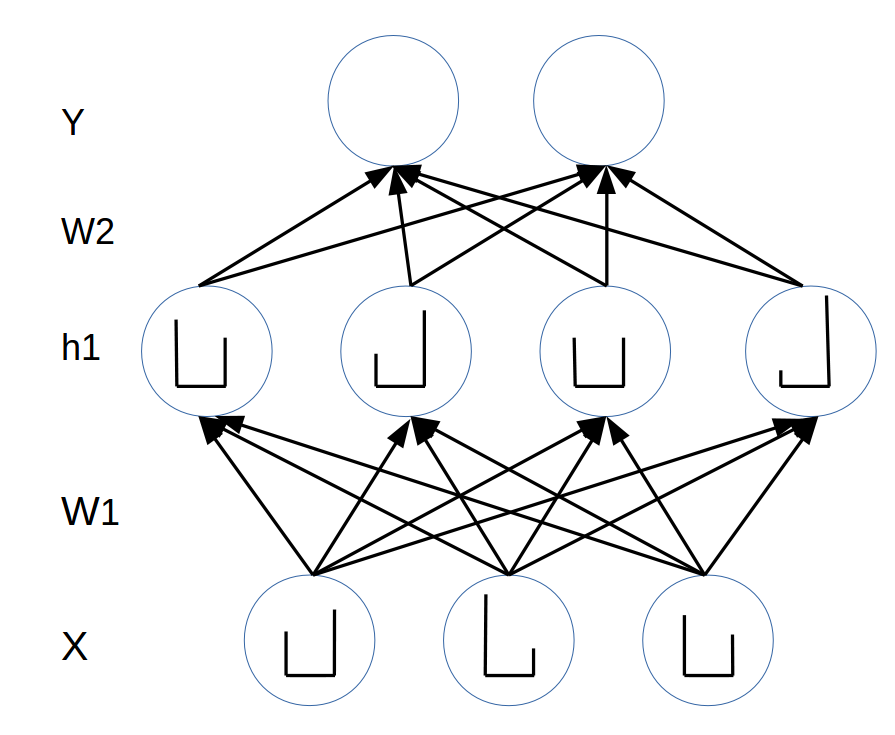
\includegraphics[width=9cm]{multi-drop}
		\caption{Different dropout rates for different hidden units in multi-drop.}		
		\label{fig:multi-drop}
	\end{center}
\end{figure}

\newpage
\subsection{Modified network architecture}
After introducing dropout and concrete dropout variational inference, we will describe the modified network architecture in this subsection. The fundamental task in this work is object classification. We choose ResNet50\cite{he2016deep} pre-trained on ImageNet as backbone for fine-tuning because of its strong ability to learn powerful representation for images. However, there is no dropout in original version of ResNet50. If we want to employ dropout variational inference to obtain reliable uncertainty estimation, dropout should be inserted into the network. In this work, we add three fully connected layer with 1024 hidden units , which are initialized from scratch, before the output layer whose dimension needs to be set to the number of classes. Then we add concrete dropout at flatten layer, and these three new added fully connected layer, respectively.
There are three reasons why we modify the network in this way:
\begin{itemize}
	\item Because we initialize major parts of network with pre-trained weights, inserting dropout in layers initialized with pre-trained weights would destroy pre-trained features. This would lead to significant drop of performance after fine-tuning. 
	\item According to the suggestions from \cite{srivastava2014dropout}, insertion of dropout reduces the capacity of the model and thus a model with	dropout should have larger capacity than one without dropout. Therefore we add three more fully connected layers to make sure that our model possesses large enough model capacity.
	\item As we have introduced in previous sub-sections, weights are major part of variational parameters. Therefore to have more weights can enhance the flexibility and capacity of approximate distribution family, which improves the quality of approximation.  
\end{itemize}

From figure \ref{fig:modified_net}, we can see the sketch of our modified network architecture. More concretely, we can interpret major parts of network, which do not have dropout inserted, as a deterministic feature extractor. On the other hand, for layers with dropout inserted work as a probabilistic classifier based on aforementioned Bayesian interpretation of dropout. In training, these two parts are trained jointly in order to achieve a better balance and more optimal results. In testing, we need to marginalize possible parameters according to posterior distribution. Layers with dropout should be sampled and run multiple times to produce a predictive distribution of output class.
\begin{figure}[h!]
	\begin{center}
		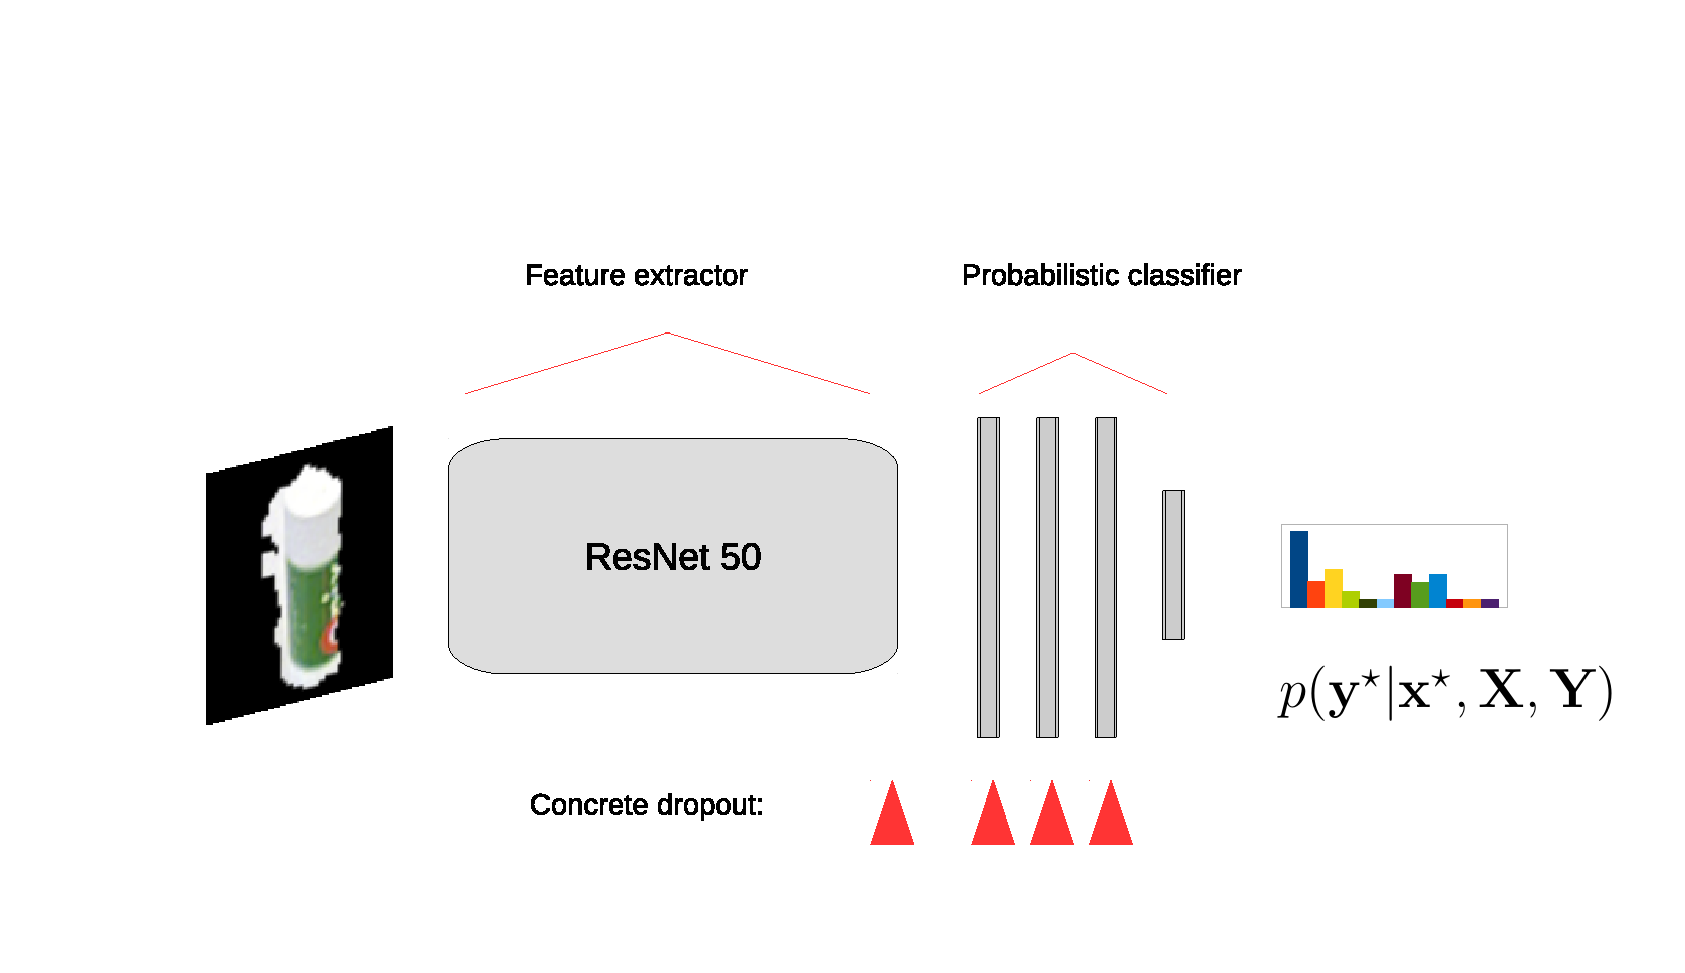
\includegraphics[height=7.5cm, width=16cm]{network}
		\caption{Modified network architecture.}		
		\label{fig:modified_net}
	\end{center}
\end{figure}


\newpage
\section{Laplace approximation}
\subsection{Introduction}
In this section, we introduce another method to approximate the real posterior distribution over weights of deep neural nets. This method is called Laplace approximation\cite{bishop2006pattern}, which is one deterministic approximation because only point estimation of model parameters instead of the learned variational parameters is required. The idea behind that is to put a Gaussian approximation on the maximum a posterior point estimate of the model parameters, which is one mode of posterior distribution. The reasons why we consider this method are as following:
\begin{itemize}
	\item it has easy compatibility to existing network. To perform Laplace approximation, we only need one point estimation of model parameters which is already available for most of architectures. That also means, we do not need modify the training phase and we can have approximation of the true posterior for all trained models.
	\item it can capture relationship between model parameters. As is mentioned in the first chapter, most of approximation approaches make assumption that parameters are independent to each other for simplicity and computation burden. That could be a quite strong restrictions on the approximation leading to bad performance.
\end{itemize}

In the following, we introduce the basic idea of Laplace approximation and further introduce its scalable version for deep neural network based on Kronecker factor approximation.

Assume we have a point estimate of model parameters via maximum a posterior estimation:
\begin{equation}
\begin{aligned} \label{point estimate}
\bld \omega^\star &= argmax_{\bld \omega}\{p(\bld \omega|\bld Y,\bld X)\} \\
&= argmax_{\bld \omega}\{\frac{p(\bld Y|\bld X, \bld \omega) p(\bld \omega)}{p(\bld Y | \bld X)}\} \\
&= argmax_{\bld \omega}\{p(\bld Y|\bld X, \bld \omega) p(\bld \omega)\}
\end{aligned}
\end{equation}


After taking a second order Taylor expansion of the logarithm of of posterior distribution $p(\bld \omega | \bld Y, \bld X)$ around its mode $\bld \omega^\star$, we have:

\begin{equation}
\begin{aligned} \label{taylor expansion}
\text{log} p(\bld \omega| \bld Y, \bld X) &\approx 
\text{log}p(\bld \omega^\star|\bld Y, \bld X) + \\
&(\bld \omega - \bld \omega^\star)^T\frac{\partial \text{log} p(\bld \omega| \bld Y, \bld X)}{\partial \bld \omega} + \\
&\frac{1}{2}(\bld \omega - \bld \omega^\star)^T\frac{\partial^2\text{log} p(\bld \omega |\bld Y, \bld X)}{\partial \bld \omega^2}(\bld \omega - \bld \omega^\star)\\
&= \text{log}p(\bld \omega^\star|\bld Y, \bld X) - \frac{1}{2}(\bld \omega - \bld \omega^\star)^T\bld H(\bld \omega - \bld \omega^\star)
\end{aligned}
\end{equation}


where 
\[
\begin{aligned}
\bld H &= -\frac{\partial^2\text{log} p(\bld \omega|\bld Y, \bld X)}{\partial \bld \omega^2}\\
&=-\frac{\partial^2\text{log}\big(p(\bld Y|\bld X, \bld \omega)\big)}{\partial \bld \omega^2} - \frac{\partial^2p(\bld \omega)}{\partial\bld \omega^2}
\end{aligned}
\]

which is negative Hessian of the log posterior. The first order term in equation \ref{taylor expansion} vanishes because we expand the function around a local maximum $\bld \omega^\star$, where the first derivative is zero. If we exponentiate this equation, we can get the following Gaussian-like functional form: 

\begin{equation}
\begin{aligned}\label{gaussian form}
p(\bld \omega | \bld Y, \bld X) \propto p(\bld \omega^\star|\bld Y, \bld X)\exp\{-\frac{1}{2}(\bld \omega - \bld \omega^\star)^T\bld H (\bld \omega - \bld \omega^\star)\}
\end{aligned}
\end{equation}

which means $\bld \omega \sim \mathcal N(\bld \omega^\star, \bld H ^{-1})$. Therefore, we can obtain a Gaussian approximate distribution with local maximum $\bld \omega^\star$ as mean and inverse of negative Hessian as covariance matrix.

We assume a Gaussian prior for weights. Then it's easy to know that the second order derivative of prior distribution term $\frac{\partial^2p(\bld \omega)}{\partial\bld \omega^2}$ is a identity matrix multiplied by regularization coefficient. And the non-trivial part is the first term, second derivatives of log likelihood. To make the explanation uncluttered, we define the Hessian of log likelihood with $\bld{\hat{H}}$ instead:

\[
\bld{\hat{H}} = -\frac{\partial^2\text{log}\big(p(\bld Y|\bld X, \bld \omega)\big)}{\partial \bld \omega^2}
\] 

However, we should note that for a large training set, it's always infeasible to analyze the gradients or Hessian exactly. To resolve this, normally we estimate the expectation of gradients or Hessian in each mini-batch. That means we need to estimate Hessian with empirical average Hessian computed in mini-batches:
\[
\bld{\hat H} \approx N\mathbb E_{p(\bld Y, \bld X)}[\bld{\hat{H}}]
\]
where $N$ is size of training samples, and 
\begin{equation} \label{expected hessian}
\mathbb E_{p(\bld Y, \bld X)}[\bld{\hat{H}}] \approx -\frac{1}{K}\sum_{k}\big[\frac{1}{M}\sum_{i}\frac{\partial^2\text{log}\big(p(y_{ik}|\bld x_{ik}, \bld \omega)\big)}{\partial \bld \omega^2}\big]
\end{equation}

where $K$ is total number of mini-batch, and $(y_{ik}, \bld x_{ik})$ is the $i$-th training data sample in $k$-th mini-batch. 

\paragraph{Fisher information matrix} is equivalent to the expected negative Hessian of exponential family log probability. Therefore we can use Fisher information matrix as replacement of expected Hessian for the log likelihood term. The derivation of equivalence between expected Hessian and Fisher matrix is straightforward. We define Fisher matrix $\bld F$ in the following:
\begin{equation}
\begin{aligned}\label{Fisher}
\bld F &= \mathbb E_{p(\bld Y, \bld X)}\big[\frac{\partial}{\partial \bld \omega}\text{log}p(\bld Y|\bld X,\bld \omega)\frac{\partial}{\partial \bld \omega}\text{log}p(\bld Y|\bld X,\bld \omega)^T\big] \\
&\approx \frac{1}{K}\sum_{k}\big[\frac{1}{M}\sum_{i}
\big(\frac{\partial}{\partial \bld \omega}\text{log}p(y_{ik}|\bld x_{ik},\bld \omega)\frac{\partial}{\partial \bld \omega}\text{log}p(y_{ik}|\bld x_{ik},\bld \omega)^T\big)\big]
\end{aligned}
\end{equation}

We include the derivation of equivalence between negative expected Hessian and Fisher matrix for case that parameter is scalar in appendix \ref{appedix:fisher_matrix}, which can be generalized to case for vector.
Therefore we can obtain 

\begin{equation} \label{fisher hessian}
\bld{\hat H} \approx N\bld F
\end{equation}

Actually, to compute outer product of gradients is feasible. But to compute the empirical average of outer product we need to save values with amount quadratic to the number of model parameters which induces large storage overhead. More than that, to inverse this matrix, the computation complexity is cubic of dimensionality of this matrix which is the number of model parameters which is also infeasible because the number of parameters in deep neural nets can reach million easily. Therefore an efficient approximation for Fisher matrix is required. 

\subsection{Scalable Laplace approximation for neural network}
In order to mitigate the computational burden in Laplace approximation above, \cite{ritter2018scalable} proposes to use Kronecker-factored approximation curve(KFAC) in \cite{martens2015optimizing} to approximate the Fisher matrix and perform Laplace approximation for neural network.




\chapter{Conditional random field}
Graphical models allow us to encode relationships between multiple variables using a concise, well-defined language. Because it's hard to solve the problems deterministically in real world. \textit{Probabilistic graphical model}(PGM)\cite{koller2009probabilistic} can assist in this case by encoding a joint or conditional probability distribution with graph, which means that PGM can encode the relationships between multiple random variables. 

The various types of PGM differ by the graph structure and the conditional independence assumptions. There are mainly two types, directed and undirected graph. Directed graphical model which is also called Bayesian network, specifies the family of distributions by means of directed acyclic graph and its joint distribution is factorized over each node which is a random variable with probability distribution conditioned on its parents. On the other hand, undirected graphical model, also known as Markov random field has undirected acyclic or cyclic graph. Its joint distribution is factorized over cliques, which is a fully-connected subgraph within the graph. This means, the marginal probability distribution in undirected graphical model is not normalized over nodes, but over cliques. 

In a object recognition task, the input is set of images and output is set of predicted labels. Because the dimensionality of input is always large so that it's difficult to model it directly. Nevertheless, we want to exploit the contextual relationship between different objects. To this end, it's better to just model the relationship between output random variables, which obey the conditional distribution of output given input. \textit{Conditional random field}(CRF), first proposed by \cite{lafferty2001conditional}, is a suitable model for this purpose. In this chapter, a concise introduction of CRF is given, including definition, learning and inference in the following subsection.
 
\section{Definition}
CRF can model the conditional distribution of a set of output random variables $\bld y$ given a set of inputs $\bld x$, that is $p(\bld y | \bld x)$. In the scope of scene object recognition problem, assume we have multiple objects in one scene denoted by $\bld x = [x_1, ..., x_n]$ and their labels $\bld y = [y_1, ..., y_n]$. We want to learn $p(\bld y | \bld x)$ with CRF and make predictions for unseen data.  

To formulate the problem clearly, we denote the set of output random variables by $\bld y$ and overall output domain by $\mathcal{Y}$. CRF for one scene $\bld x$ is defined by a graph $\mathcal{G} = (\mathcal{V}, \mathcal{E})$, where a set of nodes $\mathcal{V}$ representing the random variables in $\bld y$, and a number of undirected edges $\mathcal{E}\subseteq\mathcal{V}\times\mathcal{V}$ representing the dependencies between random variables. The output domain of CRF is the product of individual variable domains $\mathcal{Y}_i$ so that we have $\mathcal{Y} = \underset{i\in V}{\times} \mathcal{Y}_i$, where $\mathcal{Y}_i = \mathcal{L}$, which is a set of all possible labels. With these notations, we can define the probability distribution of $\bld y$ conditioned $\bld x$ with model parameter $\bld \theta$ as 
\begin{equation}
\label{crf}
\begin{aligned}
p(\bld y|\bld x; \bld \theta) = \frac{1}{Z(\bld x, \bld \theta)}\prod_{c\in\mathcal{C}}\psi_{c}(y_c, x_c, \bld \theta)
\end{aligned}
\end{equation}
where $\mathcal{C}$ is the set of cliques of graph $\mathcal{G}$, and $Z(\cdot)$ is normalizer to make sure $\sum_{\bld y \in \mathcal{Y}}p(\bld y | \bld x; \bld \theta) = 1$, which is also called partition function. $\bld \theta$ stands for the parameters of CRF to be tuned during training phase. $\psi_c(\cdot)$ is called potential function or factor which encodes the contribution of clique $c$ to the total density. The order of number of random variables in clique $c$ can be arbitrary number. However, for computational reason, we only consider factor with number of random variables up to two in normal case. The first order potential is called \textit{unary} potential which means that the clique of this kind of potential contains only one random variable, that is $\psi_i(y_i, x_i, \bld \theta)$. Unary potential can be treated as the likelihood that a label is assigned to this random variable independently to others. The second order potential is called pairwise potential $\psi_{i,j}(y_i,y_j, x_i, x_j, \bld \theta)$ characterized by edges in the graph. This kind of potential states the compatibility of two random variables $(y_i,y_j)$ being assigned to a certain pair of categories. 

To make the explanation more clear, we illustrate a simple example in figure \ref{crf}, we ignore $\bld \theta$ here and explain it later and use $\psi_{i,j}$ for $\psi_{i,j}(y_i,y_j,x_i,x_j)$ to make expression of conditional probability uncluttered:

\[
\begin{aligned}
p(y_1, y_2, y_3, y_4) &= \frac{1}{Z(x_1, x_2, x_3, x_4)}\psi_1\psi_2\psi_3\psi_4\psi_{1,4}\psi_{1,2}\psi_{2,3}\psi_{2,3}\psi_{1,2,4} \\
&=\frac{1}{Z(x_1, x_2, x_3, x_4)}\psi_1\psi_2\psi_3\psi_4\psi_{1,4}\psi_{1,2}\psi_{2,3}\psi_{2,3}
\end{aligned}
\]

where the transformation from first line to second line comes from the ignorance of potentials with order higher than two.
\begin{figure}[H]
	\begin{center}
		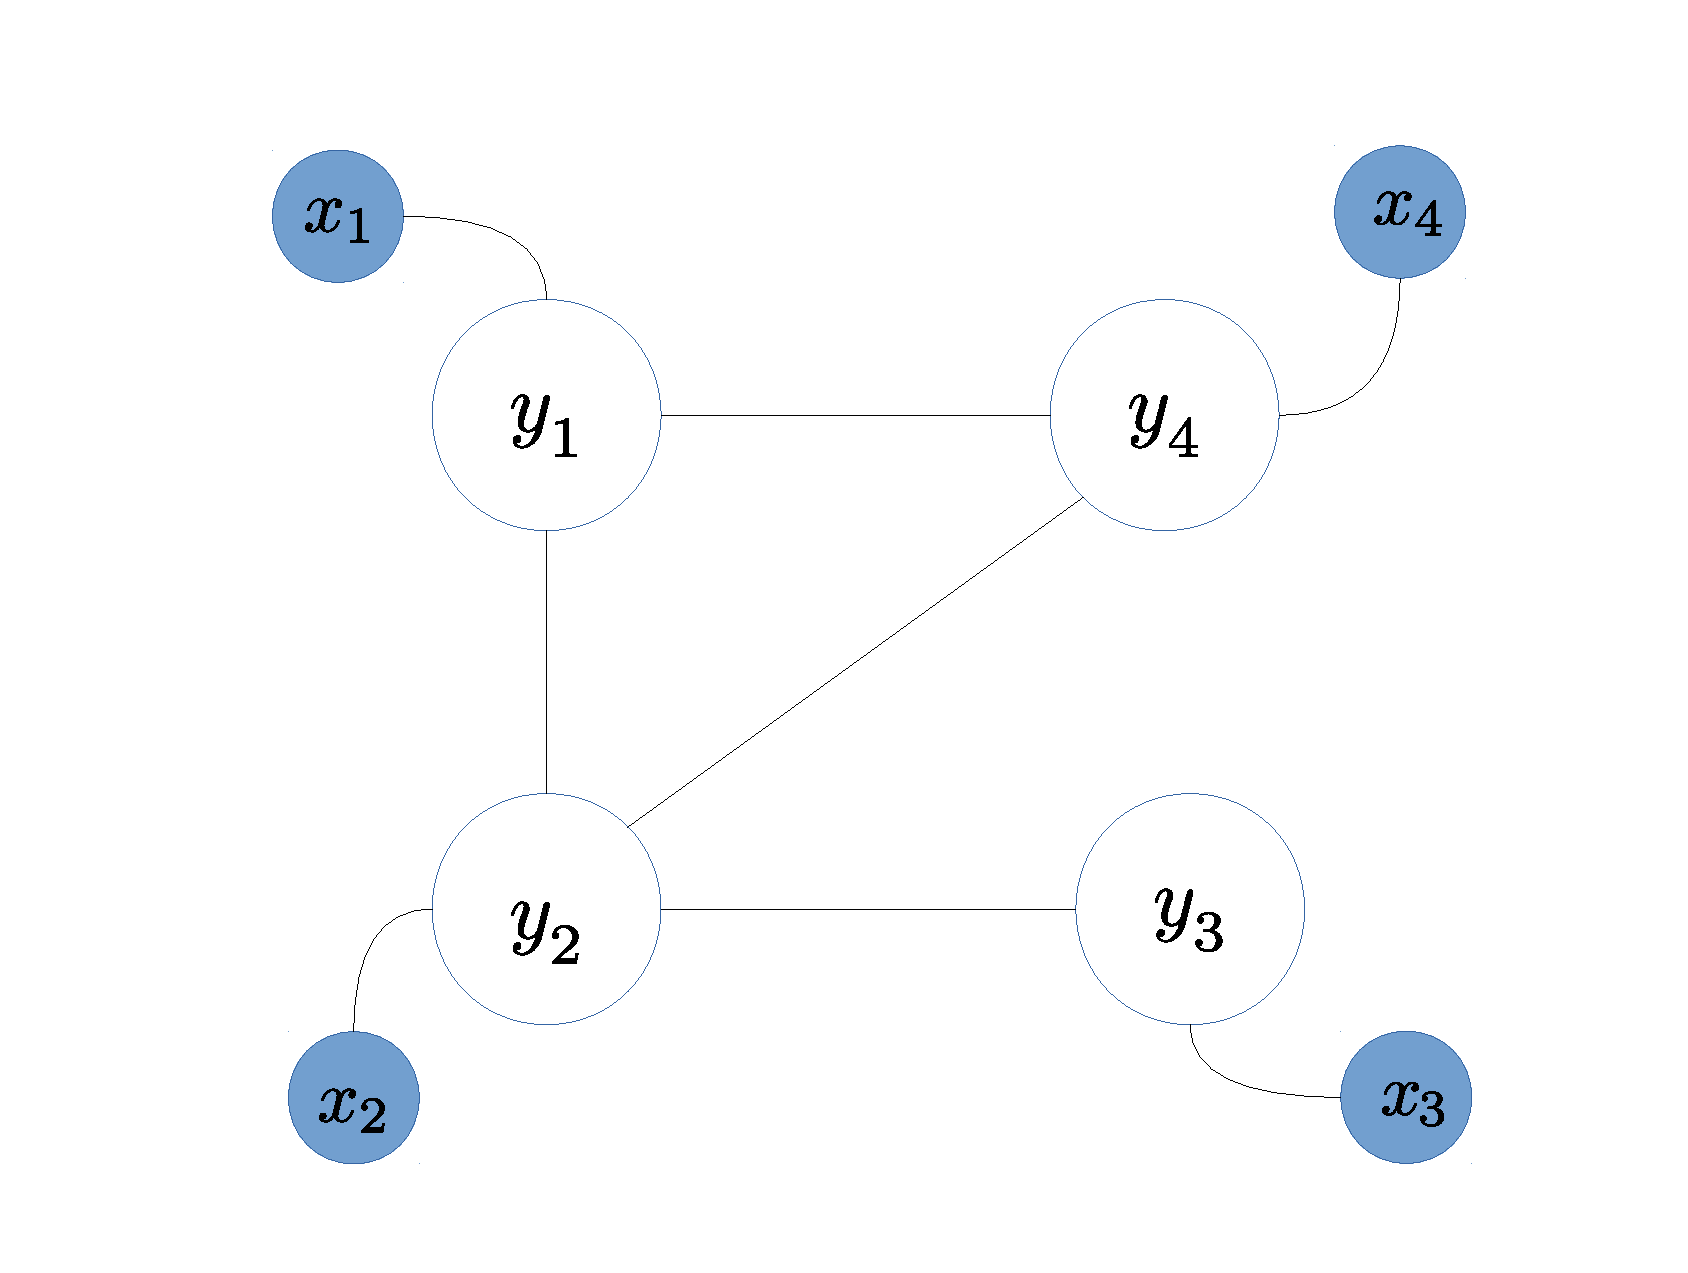
\includegraphics[height=8.5cm, width=11.5cm]{crf.eps}
		\caption{Simple example of conditional random field.}		
		\label{crf}
	\end{center}
\end{figure} 
According to Hammersley-Clifford theorem \cite{hammersley1968markov}, the the factors must be always positive, we can employ log-linear models for the potential functions, which results in:
\begin{equation}
\label{crf_potential}
\begin{aligned}
p(\bld y | \bld x; \bld \theta) &= \frac{1}{Z(\bld x, \bld \theta)}\prod_{c\in \mathcal{C}}\exp(\langle\phi(x_c, y_c), \bld \theta\rangle)\\
&=\frac{1}{Z(\bld x, \bld \theta)}\exp(\sum_{i\in V}\langle\phi_u(x_i, y_i), \bld{\theta}_u\rangle + \sum_{(i,j)\in \mathcal{E}}\langle\phi_p(x_i, x_j, y_i, y_j), \bld{\theta}_p\rangle)
\end{aligned}
\end{equation}
being $\langle \cdot, \cdot \rangle$ the inner product, and $\phi(x_c, y_c)$ the sufficient statistic of the factor over clique $c$. Because we consider the potentials up to second order, only feature function for unary potential $\phi_u(\cdot)$ and feature function for pairwise potential $\phi_p(\cdot)$ are considered here. This function can also be treated as feature function which extracts feature of the data over clique. 

Now we have made assumptions of graph structure and conditional dependency for the graph. This can be interpreted as a filter of a probability distribution family. Only the class of probability distribution that satisfies these assumptions such as up to second order potentials can be expressed and learned with this graph. To further identify different probability distribution in this class, we need to parameterize it and identify it with specific parameters which can learned during training. 

\paragraph{Parametrization} of the probability distribution is expressed explicitly in Eq.\ref{crf_potential}. This means that the dimension of the parameter in each kind of potential should be the same as the dimension of feature function. In this work, the feature function should be a function of input and class label, while the feature function can also be the function of only input and weight should be defined as matrix whose output dimension is the number of class serving as a linear mapping. In this work, we only consider the former case.

Regarding \textbf{unary feature}, we utilize the probability vector $p(y_i|x_i)$ which is predictive likelihood from a discriminative classifier which is a deep neural network in this work. 

\paragraph{Pairwise feature} in this work is quite simple context cue in the scene which is defined as binary co-occurrence matrix $\bld H(y_i,y_j)$. If one category occurs with another category in the same scene, then the corresponding entry in the matrix is filled with 1, otherwise 0. 

Although obtaining this pairwise feature requires knowing the ground truth labels of objects in the scene, it still makes sense in the application of this work. Because we use T-LESS dataset which will be introduced in the experiment part, each of scene images in this dataset contains multiple industrial-relevant texture-less objects, some of them are combination of objects of other categories. We want to simulate the situation that, we treat each scene as one product which is composed of multiple sub-parts. Because we know the product, and thus we also know the real labels of components of this product which is corresponding to the co-occurrence of objects in this scene and our goal is to classify the components with help of this contextual information.

Based on these two kinds of features, we have the formulation of likelihood function of CRF model for one scene as follows:
\begin{equation}
\label{crf_used}
p(\bld y|\bld x; \bld \theta) = \frac{1}{Z(\bld x, \bld \theta)}\exp(\theta_u\sum_{i\in V}p(y_i|x_i) + \theta_p\sum_{(i,j)\in \mathcal{E}}\bld H(y_i,y_j))
\end{equation}
where $\bld \theta = \{\theta_u, \theta_p\} \in \mathbb{R}^2$.

\section{Learning}
The most popular approach is estimate $\bld \theta$ is maximum likelihood estimate(MLE). The likelihood for one scene is defined in Eq.\ref{crf_used}. Normally we have large size of scenes in training set where each of them contains multiple objects. We denote training set by $\mathcal{D} = [d_1, ..., d_m]$, where each scene is represented by $d_i = (\bld x^i, \bld y^i)$. For each scene, we create a CRF model for it. Therefore we can denote the whole set of graph by $\bld{\mathcal{G}}=[\mathcal{G}_1, ..., \mathcal{G}_m]$, where $\mathcal{G}_i = (V_i, \mathcal{E}_i)$. This is consistent to previous notations when we make little modifications for $\bld x$ and $\bld y$: $\bld x^i = [x^i_1, ..., x^i_n,]$ and $\bld y^i = [y^i_1, ..., y^i_n]$. For computational convenience and stability, negative log likelihood as objective function is always employed. The objective in MLE on training set is defined as fallows:
\begin{equation}
\label{crf_obj}
\mathcal{NLL}(\bld \theta; \mathcal{D}) = -\sum_{i=1}^{m}\big(\theta_u\sum_{j\in V_i} p(y_j^i|x_j^i) + \theta_p\sum_{(j,k)\in\mathcal{E}_i}\bld H(y_j^i, y_k^i)  - Z_l(\bld x^i; \bld \theta)\big)
\end{equation}     
where 
\begin{equation}
\label{log_partition_func}
Z_l = \log
\big(
\sum_{\bld y^i \in \mathcal{Y}} 
\big( 
\theta_u\sum_{j\in V_i}p(y_j^i|x_j^i) + \theta_p\sum_{(j,k)\in \mathcal{E}_i}\bld H(y_j^i, y_k^i) 
\big) 
\big)
\end{equation}

With this expression, our problem is defined in the following form with MLE:
\begin{equation}
\label{crf_nll_opt}
\bld \theta^\star = \underset{{\bld \theta}}{argmin} \big[\mathcal{NLL(\bld \theta; \mathcal{D})}\big]
\end{equation}

The log likelihood function of CRF is proved to be concave \cite{koller2009probabilistic}, which means the local optimizer is also the global optimizer although it's not unique. To optimize this objective w.r.t. the model parameters on dataset with large size, we can employ stochastic gradient descent (SGD), which requires to calculate the gradient of object w.r.t. the model parameters $\bld \theta$. The gradients can be computed as follows, where we use $\bld \theta$ to represent parameters in order to make the expression clear:
\begin{equation}
\label{crf_grad}
\frac{\partial}{\partial \bld \theta} \mathcal{NLL}(\bld \theta; \mathcal{D}) = -\sum_{i=1}^{m}
\big(
\phi(\bld x^i, \bld y^i) - 
\mathbb{E}_{p(\bld y|\bld x^i;\bld \theta)}
\big[\phi(\bld x^i, \bld y)\big]
\big)
\end{equation}
where the expectation $\mathbb{E}_{p(\bld y|\bld x^i;\bld \theta)}
\big[\phi(\bld x^i, \bld y)\big]$ stands for the partial derivative of the log-partition function, which is retrieved by:
\begin{equation}
\label{exp_log_part}
\mathbb{E}_{p(\bld y|\bld x^i;\bld \theta)}
\big[\phi(\bld x^i, \bld y)\big] = \sum_{\bld y\in\mathcal{Y}}p(\bld y|\bld x^i;\bld \theta)\phi(\bld y, \bld x^i)
\end{equation}
The gradients of parameters corresponds to the difference between the empirical expectation of its associated sufficient statistics (the sufficient statistics of ground truth) and its expectation over the estimated probability distribution $p(\bld y|\bld x; \bld \theta)$. The goal of the optimization is to decrease the gradients until they reach zero, which means that we match of first moment of sufficient statistics over the output distribution. Therefore this way is also called moment matching.

When taking a closer look at Eq. \ref{crf_grad} and Eq. \ref{exp_log_part}, to calculate the gradients in each step of SGD, we need to compute $p(\bld y|\bld x; \bld \theta)$, which requires to compute the partition function $Z(\cdot)$. Because the number of possible assignments grows exponentially in the number of classes, it's infeasible to get a exact solution in practice. This problem also appears when we want to obtain a probability distribution(marginal inference) instead of a single prediction(MAP inference) in testing time. To compute the probability distribution in probabilistic modeling always refers to as inference. There are a bunch of research works focusing on inference. Because the CRF model in this work is fully connected, we adopt a popular and effective approach which is called loopy belief propagation and introduced in next subsection. This approach can provide a approximation to the log-partition function $Z_l(\cdot)$, which is required in \ref{exp_log_part} and to the marginal probability distribution of random variables in $\bld y$ to be plugged in \ref{crf_grad} in the graph with cycles and exact solution in graph without cycle.


\section{Inference}
Loopy belief propagation introduced by \cite{pearl2014probabilistic}, also known as sum-product algorithm, is a popular approach for probabilistic inference in graphical models. Briefly, this approach is based on the exchange of statistical information among the nodes in the graph according to their relationships. The core idea behind that is for each node in the graph to maintain its belief, which is a $k$-dimensional vector $\bld b(y_i)$ if the node is discrete random variable where $k$ is the number of class. The $i$-th entry of this vector indicates the probability that $i$-th class is assigned to this node. The belief of a node evolves as it receives \textit{messages} from it neighbors. A message $\bld m_{ij}(y_j)$ sent from node $y_i$ to node $y_j$ encodes belief of $y_i$ about what class node $y_j$ should belong to. This message, in turn, based on the messages it received from all the other neighbors except for the recipient in a previous time-step.

The algorithm keeps sending messages until the graph is calibrated, which means that the messages of two consecutive iterations are less than one threshold. However, in practice, the algorithm can not calibrate or converge. A maximum number of iteration can be set to obtain satisfactory results. The messages computation is as follows:
\begin{equation}
\label{message}
\bld m_{ij}(y_j) = \sum_{y_i\in \mathcal{Y}_i}\psi_{ij}(y_i, y_j, x_i, x_j, \theta_p)\psi_i(y_i, x_i, \theta_u) \prod_{y_k\in\mathcal{N}(y_i)\backslash y_j}\bld m_{ki}(y_i)
\end{equation}
where $\mathcal{N}(y_i) \backslash y_j$ is the set of node neighbors of $y_i$ except for $y_j$. Once the iteration reaches maximum number or the graph is calibrated, we can compute the belief of each node as follows:

\begin{equation}
\label{belief}
\bld b(y_i) = \frac{1}{Z_i}\psi_i(y_i, x_i, \theta_u) \prod_{y_j\in\mathcal{N}(y_i)}\bld m_{ji}(y_i)
\end{equation}
where $Z_i$ is the normalizer of unnormalized belief of node $y_i$ to ensure the sum of marginal probability of $y_i$ is 1. 

For the implementation, we employ the library in C++ from \cite{Ruiz-Sarmiento-REACTS-2015}. However, the weights in this library are assumed to be category-independent, which means that the weights are defined as weight matrix to build a linear mapping from feature function to potential function. Therefore we need to modify the type of weights in this library in order to incorporate different type of weight defined in Eq. \ref{crf_used}, which serve as coefficient of potential function instead of a linear mapping inside the potential function. To note that the messages are initialized uniformly during loopy belief propagation.




\chapter{Experiments and Discussion}

\section{Introduction}
In this chapter, we perform different experiments for the following purposes:
\begin{itemize}
	\item to evaluate the performance of uncertainty estimation of dropout variational inference and its variants as well as Laplace approximation. Comparisons and analysis towards the results of these two kinds of approach are given.
	
	\item to evaluate performance of training a domain specific classifier, with different strategies for collecting training data including manual labeling and automatic labeling, where the latter one is chosen based on uncertainty estimation.
	
	\item to evaluate performance of classifier including context information via CRF.
\end{itemize}

Before looking into the results, we need to specify the details of experiments such as the dataset, evaluation metrics. Besides, the detailed parameters of the model will be reported in section of each experiment to avoid confusions. Models were implemented in Tensorflow\cite{abadi2016tensorflow}, and optimization was performed using RMSprop with initial learning rate of $1e^{-5}$ and L2 regularization with coefficient of $3.5e^{-6}$ as well dropout regularization with coefficient of $1.0e^{-5}$. We used early stopping with all methods, where the amount of epochs to run was determined based on performance on a validation set. We set the number of maximum epoch as 20.


\subsection{Dataset}
\paragraph{WRGBD\cite{lai2011large}} This dataset is a large-scale dataset of 300 household objects captured from multi-viewpoint. The objects are organized into 51 categories, some of categories and their subtrees. To note that category level recognition involves classifying objects with similar semantic appearance such as cereal boxes with different texture into same category, instead of just physical appearance. Instance level recognition is to classify objects with similar physical appearance to the same category. Therefore the overlapping of features between classes in category recognition is larger than that in instance recognition. More abstract and semantic concepts are expected to be learned in category recognition. Each object was placed on a turn table and captured from a systematically sampled view hemisphere with $15^{\circ}$ step in elevation (from $30^{\circ}$to $60^{\circ}$) and $2^\circ$ step in azimuth (from $0^\circ$ to $360^\circ$) (cf. figure \ref{fig:wrgbd2}). The total size of entire dataset is around $160.9\times10^3$. 

\paragraph{UniHB} To simulate application-specific situation in deployment of robots, we recorded a similar dataset by putting objects on a turn table in front of the robot and recording partial views of objects. We follow the same methodology as \cite{lai2011large} suggests for WRGBD, but with only one object instance for each category in the dataset. This analogue of WRGBD dataset is called the IAI-ODU dataset of UniHB. The size of data with elevation $45^\circ$ is around $8.6\times10^3$ and that of data with elevation $30^\circ$ and $60^\circ$ is around $17.1\times10^3$.

While the UniHB dataset's setup strives to mimic the WRGBD one, the differing capturing conditions such as different equipment and light conditions even appearances of objects, result in obvious changes in feature space, thus yielding a significant drop on classification accuracy. In addition to the existing 51 categories, there are 28 novel objects(cf. figure \ref{fig:not_in_wrgbd}) that do not belong to the 51 categories and these objects are treated as out-of-distribution(OOD) data for testing uncertainty estimation of the model. To note that data of these novel objects are recorded in a slight different way, that is, their view points are sampled with $15^{\circ}$ step in elevation (from $30^{\circ}$to $60^{\circ}$) and $5^\circ$ step in azimuth (from $0^\circ$ to $360^\circ$). The size of this OOD dataset is around $6.0\times10^3$.

% and are captured from a systematically sampled view sphere with $10^{\circ}$ step in elevation (from $85^\circ$ to $-85^\circ$) and $5^\circ$ step in azimuth

%Each test scene is captured from a systematically sampled view hemisphere with $10^{\circ}$ step in elevation (from $75^{\circ}$ to $15^{\circ}$) and $5^{\circ}$ step in azimuth.

\paragraph{T-LESS\cite{hodan2017tless}} This dataset features 30 commodity electrical parts which have no significant texture, discriminative color or distinctive reflectance properties, and often bear similarities in shape and/or size. Furthermore, a unique characteristic of the objects is that some of them are parts of others. All images were captured systematically sampled from a view sphere, resulting in around $38.0\times10^3$ training and $10.0\times10^3$ test images (cf. figure \ref{fig:tless_test}). The training images depict objects in isolation with a black background, while the test images are from twenty table-top scenes with arbitrarily arranged objects placed on table. In this work we only consider the cropped images of objects in testing scenes, resulting a testing set with size $69.5\times10^3$, while the scene context information can be exploited with conditional random field in the final experiment.

Because objects in test scenes are mostly occluded and have different background and reflectance. Therefore we employ data augmentation to improve the performance of classifier (cf. figure \ref{fig:tless_train}). Since collecting real data requires much manual effort, we want to first train classifier on synthetic data which are augmented images from 3D reconstructed CAD models(cf. figure \ref{fig:tless_train}). By comparing the real object and synthetic image, there is significantly large domain gap such as texture and details on the object, which can decrease the performance on test set greatly. Based on improved uncertainty estimation we can collect labeled data automatically, which is used to train a more accurate classifier.


 \begin{figure}[H]
 	\begin{center}
 		\includegraphics[height=9.5cm, width=16cm]{domain_diff}
 		\caption{Example of masked images of objects from 51 categories in WRGBD and UniHB dataset. In each category, the left is from WRGBD and the right is from UniHB. We randomly pick one instance for the objects of WRGBD. We can see some light and appearance difference between objects in these two datasets.}		
 		\label{fig:wrgbd2}
 	\end{center}
 \end{figure}

\begin{figure}[H]
	\begin{center}
		\includegraphics[height=6cm, width=12cm]{not_in_wrgbd}
		\caption{Example of masked images of objects from 28 categories which are not belonging to WRGBD categories, which are treated as OOD data samples.}		
		\label{fig:not_in_wrgbd}
	\end{center}
\end{figure} 

\begin{figure}[H]
		\centering
		\includegraphics[height=9cm, width=16cm]{tless_domain_diff}
		\caption{Example of object of each category after augmentation. In each thumbnail, the left image is real augmented object and the right image is synthetic augmented object.}		
		\label{fig:tless_train}
\end{figure} 

\begin{figure}[H]
	\begin{center}
		\includegraphics[height=8.2cm, width=14cm]{tless_trn_test}
		\caption{Example of object of each category in original training set and test set. In each thumbnail, the left image is real single object with black background and the right image is cropped image of object in test scene.}		
		\label{fig:tless_test}
	\end{center}
\end{figure} 

\subsection{Uncertainty measures}
For each prediction, we can obtain one predictive probability distribution from our model with equation \ref{marginalization_test}. In order to quantify uncertainty of the prediction, there are different metrics to measure the uncertainty of prediction, which are introduced in the following. We define $x^\star$ as one test data sample and $\mathcal D$ as our training set. 
\paragraph{Confidence} is defined as the maximum probability of the output predictive distribution, whose index is the class prediction.

\begin{equation}\label{confidence}	
\begin{aligned}
conf = \max_c \big[ p(y=c|x^\star, \mathcal D) \big]
\end{aligned}
\end{equation}
where $conf \in [0,1]$, $c \in \mathcal P = \{0,...,|\mathcal P|-1\}$, and $\mathcal P$ represents output space in which label is expressed as number index which is transformed into one-hot representation in computation of objective function. The larger this quantity is, the less uncertain the prediction is. 

\paragraph{Predictive entropy} is quantity that captures the average amount information contained in predictive distribution\cite{shannon1948mathematical}: 
\begin{equation}\label{entropy}	
\begin{aligned}
\mathcal H[p(y|x^\star, \mathcal D)] = -\sum_{c}p(y=c|x^\star, \mathcal D)\text{log}p(y=c|x^\star, \mathcal D)
\end{aligned}
\end{equation}
where $c$ is the possible class $y$ can take, $\mathcal H(\cdot) \in [0, \text{log}{|\mathcal P|}]$, the larger this quantity is, the more uncertain the prediction is.

\paragraph{Mutual information}
Mutual information between the prediction $y$ and the weights posterior offers a different uncertainty measure when compared with the aforementioned ones. This measure is widely used in active learning tasks\cite{houlsby2011bayesian}, which is also called Bayesian active learning disagreement(BALD). The definition of this measure is as follows:
\begin{equation}\label{mi}	
\begin{aligned}
\mathcal I[y,\bld \omega|x^\star, \mathcal D] &= \mathcal H[y|x^\star, \mathcal D] - \mathbb E_{p(\bld \omega| \mathcal D)}\big[\mathcal H[y|x^\star, \bld \omega] \big] \\
&= -\sum_{c}p(y=c|x^\star, \mathcal D)\text{log}p(y=c|x^\star, \mathcal D) \\ &+ \mathbb E_{p(\bld \omega|\mathcal D)}[-\sum_{c}p(y=c|x^\star, \bld \omega)\text{log}p(y=c|x^\star, \bld \omega)] \\
&\approx -\sum_{c}p(y=c|x^\star, \mathcal D)\text{log}p(y=c|x^\star, \mathcal D) \\ &+ \mathbb E_{q(\bld \omega)}[-\sum_{c}p(y=c|x^\star, \bld \omega)\text{log}p(y=c|x^\star, \bld \omega)]
\end{aligned}
\end{equation}
where $\mathcal I(\cdot) \in [0,\text{log}{|\mathcal P|}]$.
This quantity considers the effect of approximate posterior distribution more directly. Compared with aforementioned uncertainty measures, this one should be able to capture the model uncertainty more accurately. To think about it intuitively, this quantity measures the information gain between the entropy of predictive output distribution and the expected entropy of output distribution wr.t. weights posterior. It will be low only if the predictive distribution agrees with most of possible models(weights realizations), which means that the model is sure about its prediction. Otherwise, it will be high because most of possible models do not agree with the other models and thus the predictive distribution will be more uniform and thus has higher entropy.

\subsection{Evaluation metrics}
As is stated in \cite{gneiting2007probabilistic}, the goal of probabilistic prediction is to maximize the sharpness of predictive distribution subject to calibration. Calibration refers to the statistical consistency between the predictive probability and the occurrence of observations, which is the frequency of the event. Therefore we employ different metrics including both the accuracy and other quantities related to calibration as well as summary of accuracy and calibration. Additionally, we also employ histogram and diagram to express the results visually. While the visual one can show us the results more intuitively, the quantitative one can allow us to evaluate the results more objectively. The comparison between them may help us to examine if visual metrics are corresponding to the numerical metrics, which may provide more insights in evaluating uncertainty estimation. 

\paragraph{Uncertainty histogram} is a intuitive visual tool for analyzing the statistics of the uncertainty estimation. Compared with normal histogram, there is one difference to stress on. In order to make visual effect more clear and hence the analysis easier, \textbf{normalizer} of each type of prediction is the size of this type of predictions instead of size of all predictions. In detail, we have three types of prediction for plotting the histogram, which are:
 \begin{itemize}
 	\item \textbf{correct prediction}
 	\item \textbf{miss-classification}
 	\item \textbf{out-of-distribution(OOD)}
 \end{itemize}The range of y axis is $[0,1]$ because we normalize the number in each bin, and range of x axis is set by the range of corresponding type of uncertainty measure.

\paragraph{Reliability diagram(Calibration curve)} is another visual tool for expressing \textbf{calibration} performance of the model\cite{guo2017calibration}, which plots the frequency of success(accuracy of predictions in specific bin) as a function of confidence, which is predictive likelihood of prediction. If the model is perfectly calibrated, this function should be overlapping with the diagonal line exactly. The closer this curve is to diagonal curve, the better the calibration performance is. In order to draw the curve, we firstly group the predictions into $M$ interval bins w.r.t. confidence and then calculate the accuracy of predictions in each bin. We use $M=20$ in this work. To quantify the proximity to the diagonal curve, we use two metrics:
\begin{itemize}
	\item \textbf{Expectation calibration error(ECE)}: in order to obtain a more objective measure of calibration quality, we can compute the \textbf{expected calibration error} by computing the weighted average of difference between accuracy and confidence:
	
	\begin{equation}
	ECE = \sum_{m=1}^{M}\frac{|B_m|}{n}|acc(B_m) - conf(B_m)|
	\end{equation}
	where $n$ is the number of samples, and $acc(B_m)$ represents the accuracy of samples, $conf(B_m)$ the average predicted confidence of samples in $m$-th bin. We can see that this metric measures the inconsistency between the statistics and predictive distribution. To note that this metric only considers the calibration quality instead of accuracy. One drawback of this metric is that, because the weights are computed based on number of samples in each bin, the metric would bias if most of predictions are clustering in few bins. Then the weights of these bins are much larger than other bins and other bins with large error would be ignored. 
	
	\item \textbf{Maximal calibration error(MCE)}:
	Considering the drawback mentioned in ECE, we make use of this metric. Additionally, in high risk applications where reliable confidence measures are absolutely necessary, we may wish to take the worst case into account. It is defined as follows:
	
	\begin{equation}
	MCE = \max_m|acc(B_m) - conf(B_m)|
	\end{equation}
\end{itemize}


\paragraph{Proper scoring rules:} 
Scoring rules provides a \textbf{summary} measure in the evaluation of probabilistic forecasts. It assigns a numerical score based on the difference between predictive distribution and real distribution. 

Because we want to make predictions for the future and also have a suitable measure of the uncertainty associated with them (see \cite{gneiting2007strictly} for a review). We can define the scoring rule as a function $\mathcal S(p(y|\bld x), (y|\bld x))$ that evaluates the quality of predictive distribution $p(y|\bld x)$ relative to an event $y|\bld x \sim q(y|\bld x)$ where $q(y|\bld x)$ represents the true distribution over $(y|\bld x)$. Consequently, the expected scoring rule is:

\begin{equation}\label{scoring rule}
	\mathcal S(p, q) = \int q(y| \bld x) \mathcal S(p,(y|\bld x))dy
\end{equation}

$\mathcal S(p,q)$ is proper if $\mathcal S(p,q) \leq S(q,q)$, with equality holds if and only if $p(y|\bld x) = q(y|\bld x)$. Here we adopt two simple and famous proper scoring rules in which the less it is, the better the performance is:
\begin{itemize}
	\item \textbf{averaged negative log likelihood(NLL)}:NLL is a popular metric for evaluating predictive uncertainty	\cite{quinonero2005evaluating}. This metric considers aforementioned confidence as likelihood. The smaller this metric is, the better the predictive distribution is.
	
	\begin{equation} \label{nll}
		NLL = -\frac{1}{|\mathcal D_{test}|}\sum_{i=1}^{|\mathcal D_{test}|}\text{log}(p(y_i = c_i|\bld x_i))
	\end{equation}
	where $c_i$ is the ground truth label for $\bld x_i$.	
	\item \textbf{Brier score} is the mean squared error between the target distribution(one-hot encoding label) and predictive distribution:
	
	\begin{equation} \label{bs}
	BS = -\frac{1}{|\mathcal D_{test}|}\sum_{i=1}^{|\mathcal D_{test}|}(\bld y^{gt}_i - p(\bld y_i|\bld x_i))^2
	\end{equation}
	where $\bld y^{gt}_i$ is the one-hot encoding ground truth label for $\bld x_i$. 
	
\end{itemize}

\paragraph{Separability metrics:} In addition to the summary metrics of predictive probability. We are also interested in the separability between different types of predictions, which can assist the down-stream tasks if they are highly separable (e.g. separate correct predictions and false predictions or out-of-distribution data to improve robustness of system and provide more safety guarantee). To note that, we treat the correct predictions as positive samples in the two following metrics.
\begin{itemize}
	\item \textbf{Area under Receiver Operating Characteristic curve(AUROC)}:Since one of our goals is to choose automatically labeled data based on uncertainty estimation, it's necessary to evaluate the separability between correct predictions and false predictions or out-of distribution data predictions. ROC curve describes the relationship between true positive rate($tpr=\frac{tp}{tp+fn}$) and false positive rate($fpr=\frac{fp}{fp+tn}$). Moreover, AUROC can be interpreted as the probability that a positive samples has a greater score than a negative samples. However, the drawback of AUROC is that, the normalizers of two kinds of rate in ROC curve are independent to each other. When these two normalizers differs too much. AUROC can provide misleading conclusion. For example, if the number of negative predictions is much higher than positive one, the AUROC could still achieve a relatively high value, while in fact there are already many false positives. 
	
	\item \textbf{Area under Precision Recall curve(AUPR)}: Considering the downside of AUROC, another evaluation metric is employed, that is AUPR. AUPR describes the relationship between precision($pr = \frac{tp}{tp+fp}$) and recall($tpr=\frac{tp}{tp+fn}$), which resolves the problem of different base number. In the previously mentioned case, though the AUROC is high, the AUPR will be low because the precision is low. 
\end{itemize}


\section{Uncertainty estimation experiments}

\subsection{Experiments \RNum{1}}
In this experiments, we want to evaluate our model on a relatively easy task which is instance recognition at first. That means, the appearances of different classes as well as the out-of-distribution data are highly discriminable. To this end, we separate WRGBD dataset into two subsets based on the instance class. Subset \RNum{1} contains objects with instance class from 0 to 199 (assuming that here we use index to denote the instance label) and Subset \RNum{2} contains objects with instance class from 200 to 299. 

We train our model with objects captured in elevation $30^\circ$ and $60^\circ$ of Subset \RNum{1} (in which we split off 20\% of training set as validation set for model selection in training). The size of training set and validation set is around $71.0\times10^3$. Then we test the model on objects captured in elevation $45^\circ$ of both Subset \RNum{1} and Subset \RNum{2}. In this experiment, the objects in Subset \RNum{2} serve as out-of-distribution samples because they are not present during training. The size of test set is around $35.6\times10^3$ and that of OOD dataset is around $17.8\times10^3$. 

In this experiment, we just want to test and compare the performance of different approaches. Because the OOD data is highly different to the training set. The model should express high uncertainty when facing these data. Nevertheless, the miss-classifications should have higher uncertainty than the correct predictions because the model should be confident when it makes predictions correctly. Otherwise the model is overconfident when it's confident with its incorrect predictions, which can induce hazardous consequence in some safety-critical applications. As we can see in the figure \ref{exp1_histo}, the original ResNet50 model is highly overconfident, which assigns high confidence to nearly $50\%$ of miss-classification and nearly $30\%$ of OOD data in the highest bin. While the model with concrete dropout and multi-drop can significantly decrease these two proportions. As we can see, different uncertainty show similar trend in this experiment.

In addition to uncertainty histogram, we also plot the calibration curve of each model evaluated on both test set and OOD dataset in figure \ref{exp1_reliability}. As expected, the calibration performance of original model is much worse than those of the other two models. This result is corresponding to the results in \cite{guo2017calibration}, that the model is highly overconfident. And the concrete dropout and multi-dropout can mitigate the undesired problem significantly.

\begin{figure}[H]
	\begin{center}
		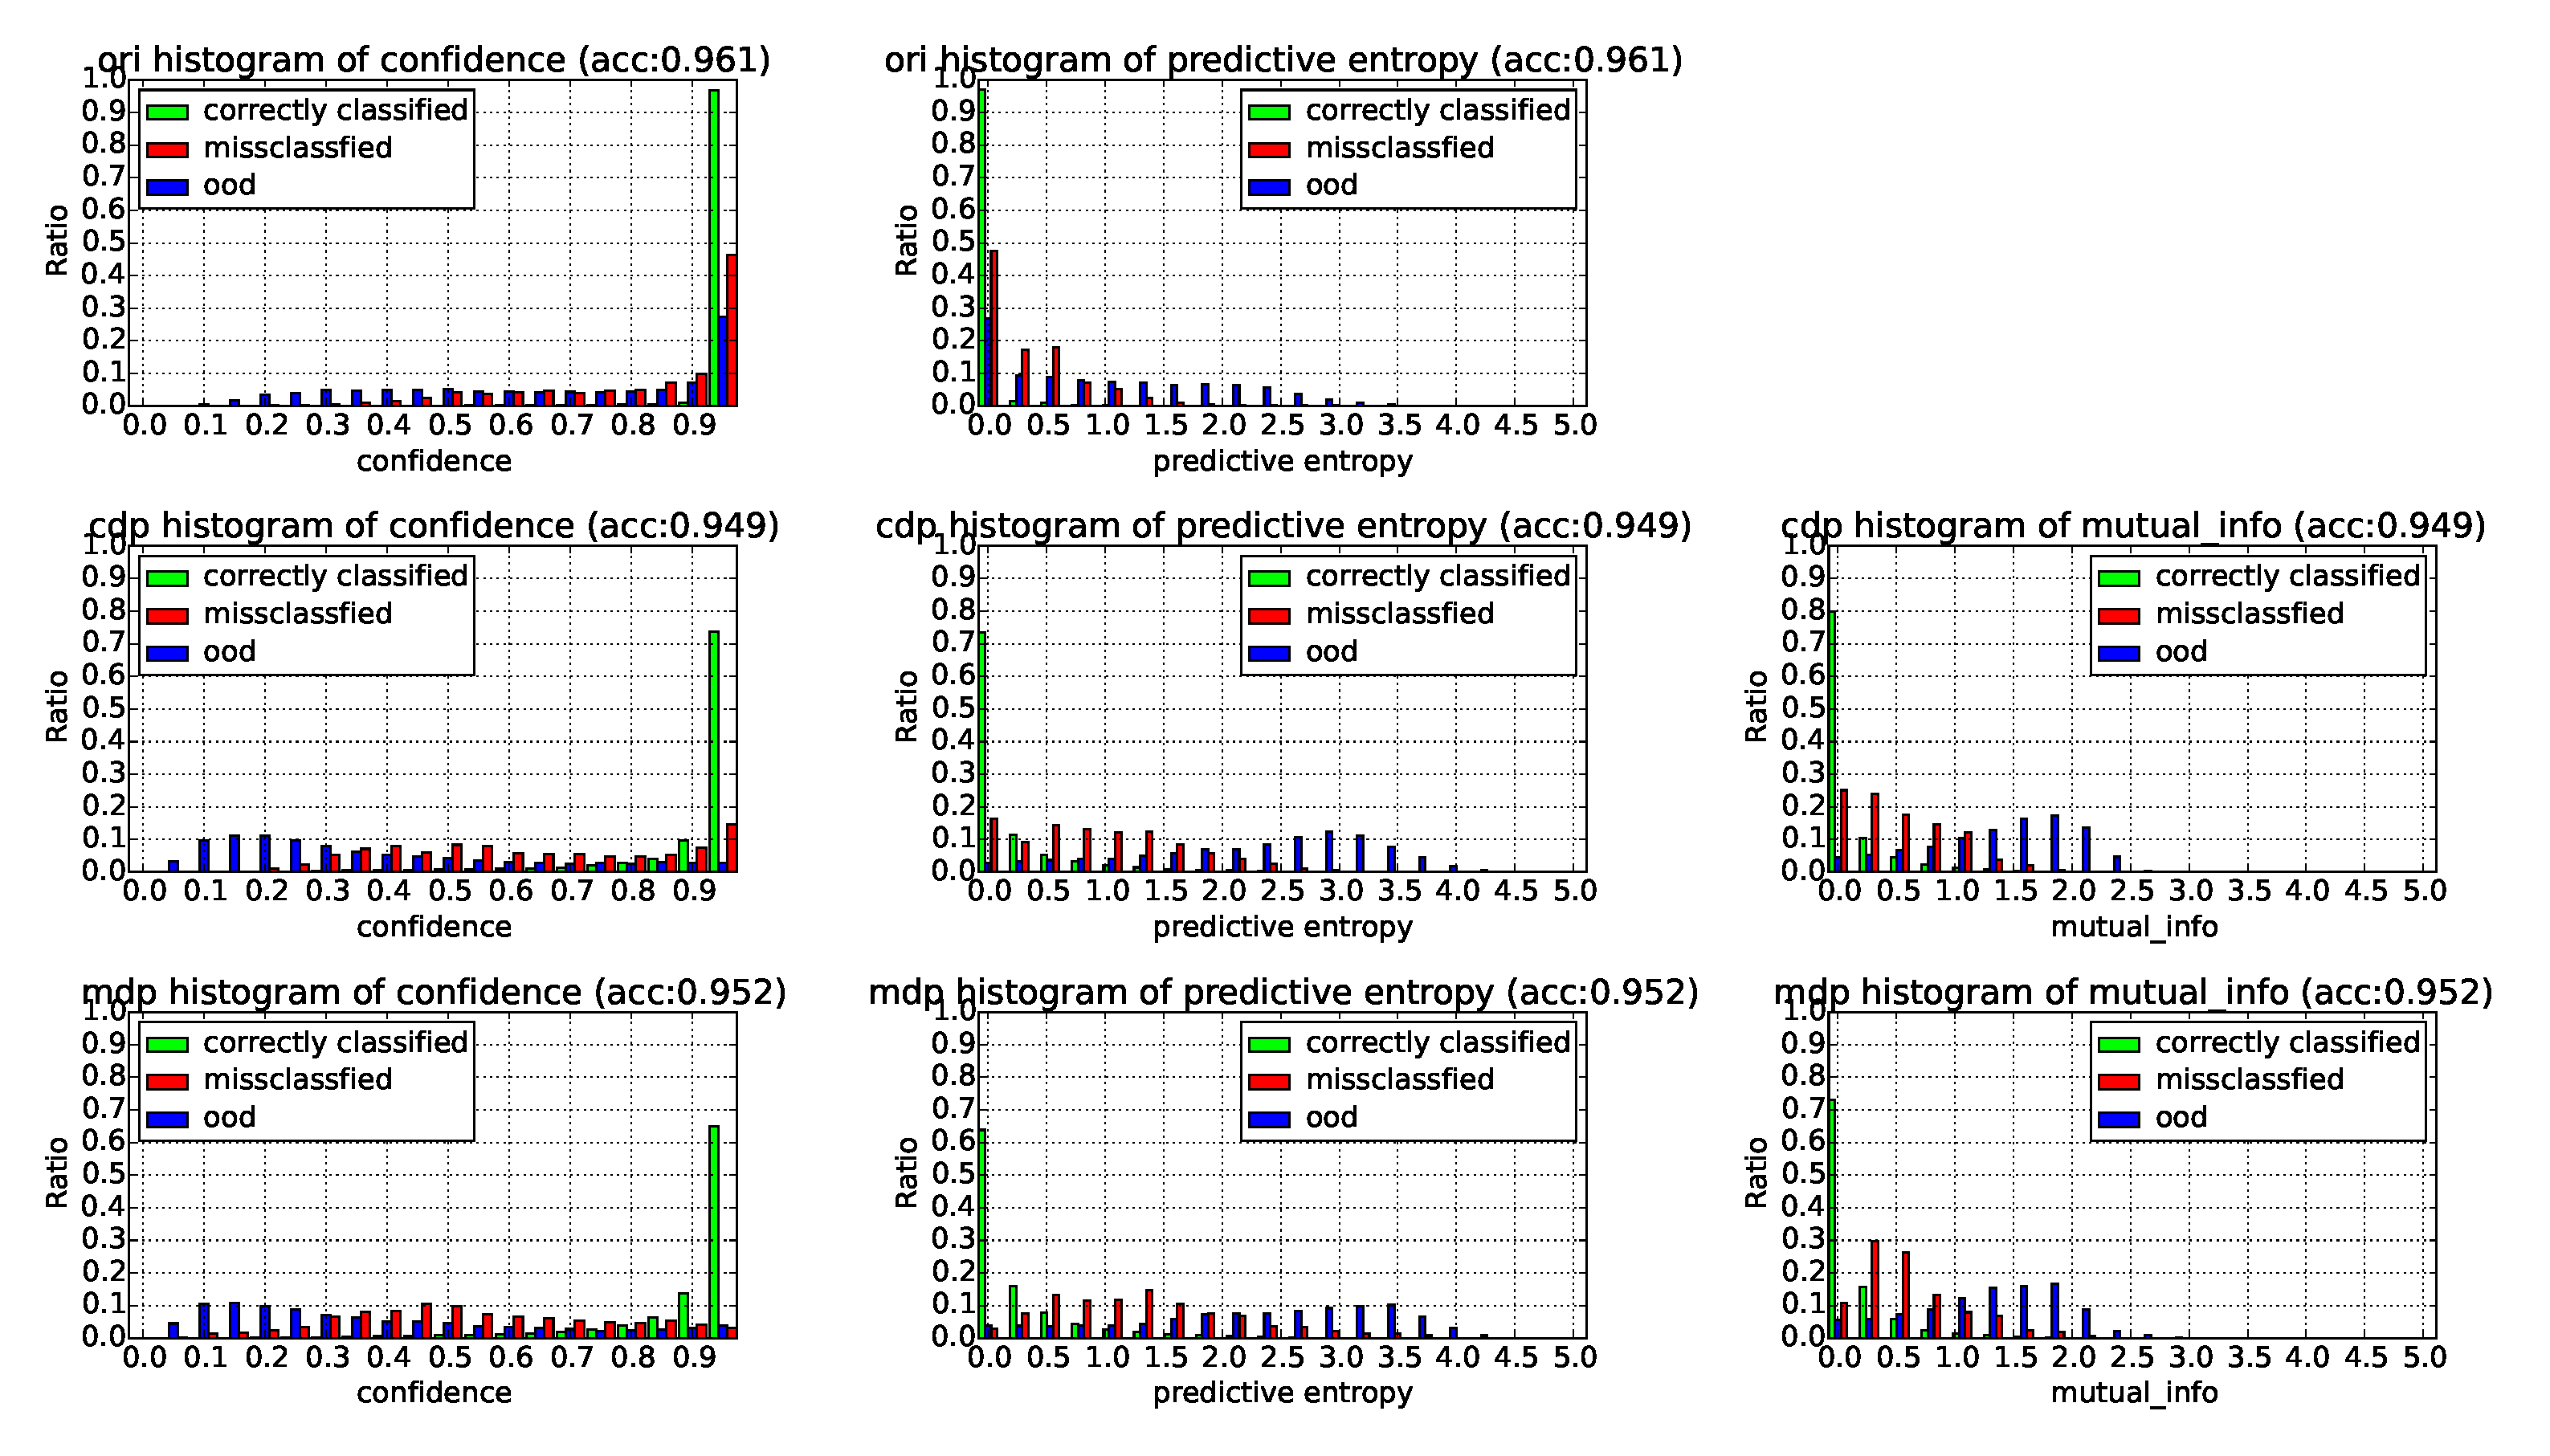
\includegraphics[height=8cm, width=16cm]{uncertainty_estimation/exp1/exp1_histo}
		\caption{Uncertainty(confidence, predictive entropy, mutual information) histograms of original ResNet50, ResNet50 with concrete dropout and ResNet50 with multi-dropout.}		
		\label{exp1_histo}
	\end{center}
\end{figure}
\begin{figure}[H]
	\begin{center}
		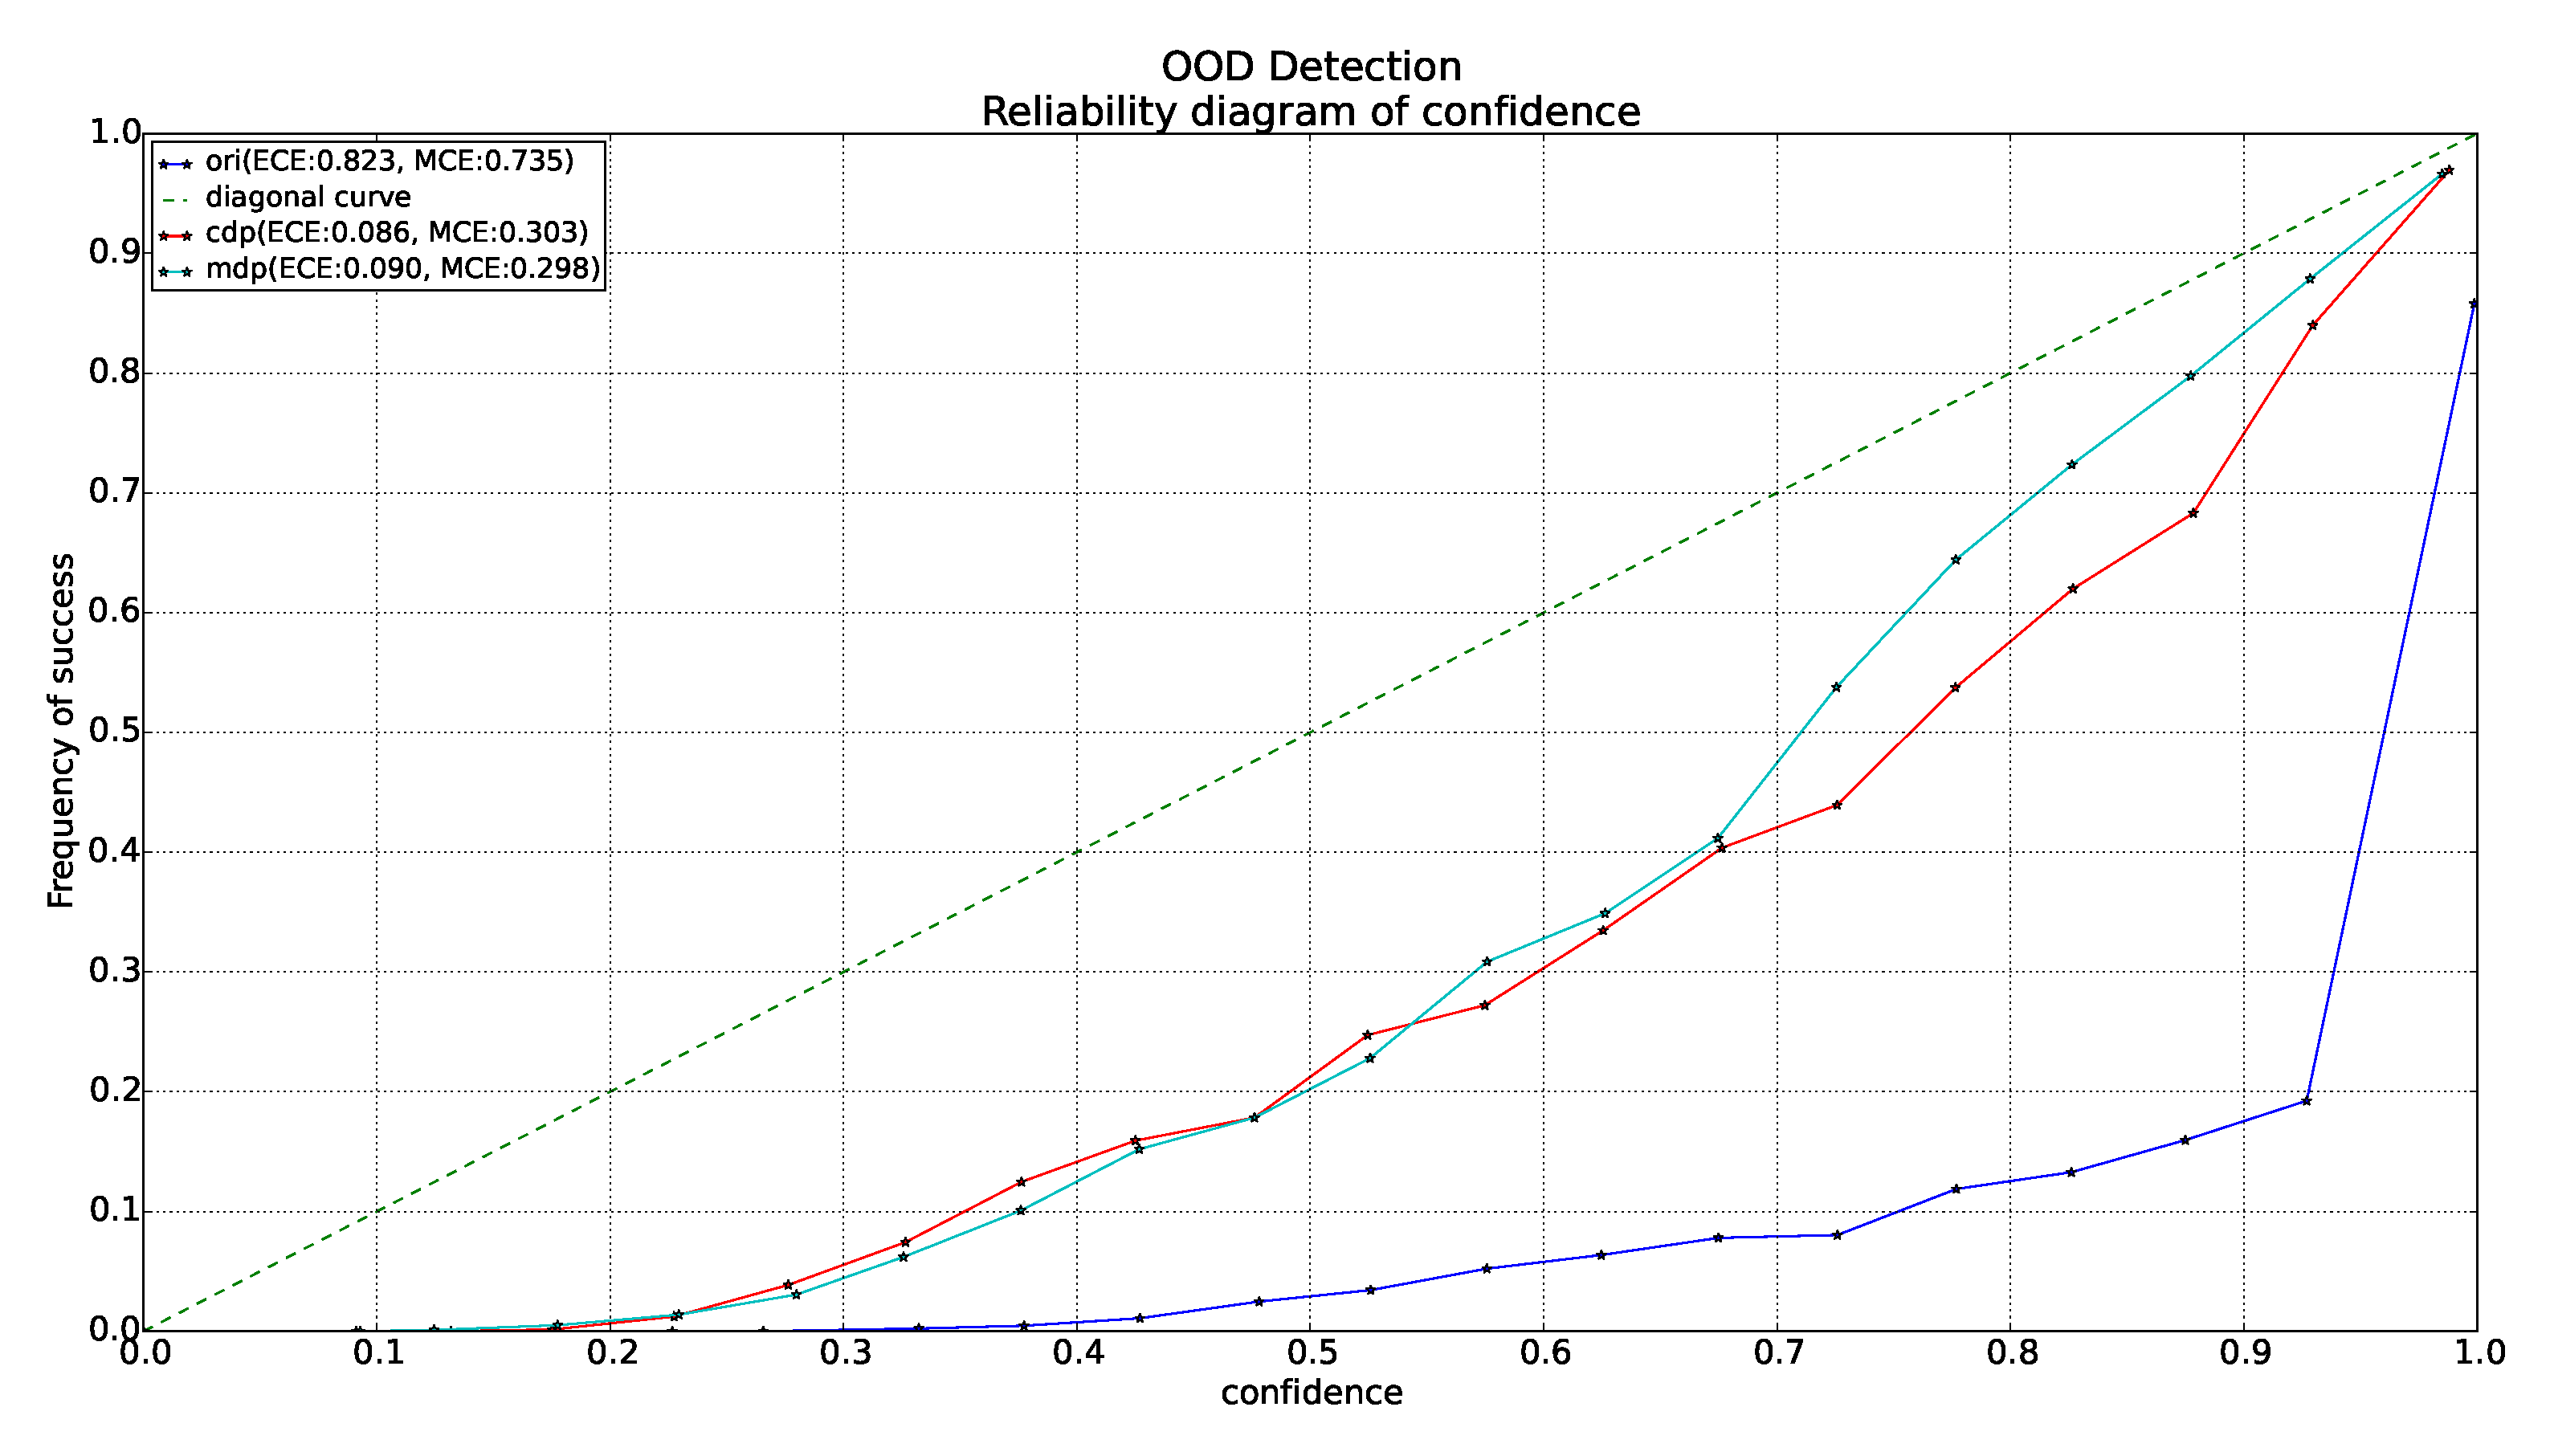
\includegraphics[height=7cm, width=12.5cm]{uncertainty_estimation/exp1/exp1_reliability}
		\caption{Calibration curves of original ResNet50, ResNet50 with concrete dropout and ResNet50 with multi-dropout.}		
		\label{exp1_reliability}
	\end{center}
\end{figure}

\newpage
\subsection{Experiments \RNum{2}}
In this experiment, we evaluate our model on a category recognition task. The difficulties are expressed in two-fold. Firstly, in this task, the model is confronted with classes with more overlapping. Second, because we want to simulate situation of deploying robots in real world scenario and facing data in real world, the UniHB dataset with domain gap(cf. figure\ref{fig:wrgbd2}) to WRGBD is used to achieve this goal. This means, the uncertainty estimation should not only be able to perform well on dataset with exactly same distribution to training set, but also to generalize well to dataset with domain gap which may decrease the accuracy significantly.

Accordingly, we use the entire WRGBD dataset including all view points, whose size is around $160.9\times10^3$, to train our model (in which we split off 20\% of training set as validation set for model selection during training). When it comes to UniHB dataset, we treat objects captured in elevation $30^\circ$ and $60^\circ$ in this dataset as \textbf{adaptation set}, whose size is around $17.1\times10^3$. We test performance of uncertainty estimation on this adaptation dataset. The images of $45^\circ$, whose size is around $8.6\times10^3$ , are used for final evaluation after we fine-tune the model with subset of adaptation set to obtain a domain specific model. The latter part will be experimented in next section. Besides, we also evaluate the uncertainty estimation on OOD dataset(cf. figure \ref{fig:not_in_wrgbd}) whose size is around $6.0\times10^3$. 

We firstly explain protocols in the following for different kinds of metric, which can help understanding the plots and extracting useful information more easily and quickly.  
\begin{itemize}
	\item The following visual metrics are chosen in one of three runs of different random seeds. The average quantitative results are given in tables following the visual metrics.
	\item The calibration curve with title "Classification" on the left is plotted \textbf{only} on predictions of test set. The one with title "OOD detection" on the right is plotted on predictions of \textbf{both} OOD dataset and test dataset.
	\item The ROC curve and PR curve measure the separability between two types of prediction.
	The ones with title "classification" on the left measure the separability between \textbf{correct prediction} and \textbf{miss-classification}. The ones with title "OOD detection" on the right measure the separability between \textbf{correct prediction} and \textbf{OOD prediction}. In all ROC curve and PR curve, correct prediction is always chosen to be positive.
	\item As is shown in uncertainty histogram, we have used three uncertainty measures. Each one has its own ROC curve and PR curve of correct prediction versus miss-classification or OOD prediction. In the following plots of ROC curve and PR curve, we only show the one with highest area under curve. In detail, \textbf{Confidence} is chosen in case of correct prediction versus miss-classification. \textbf{Mutual information} is chosen in case of correct prediction versus OOD prediction.
\end{itemize}   

\subsubsection{Comparison with Ensemble}
In this subsection, we will show the results in not only a qualitative (visual) way, but also in a quantitative way. The approaches we compare here include original version of ResNet50(ori), modified ResNet50 with concrete dropout(cdp), modified ResNet50 with multiple dropout(mdp) as well as their ensemble version. The members in ensemble are just initialized from different random seeds and no other techniques for enhancing the performance are used. In order to quantify the results more objectively, we average the results from three different random seeds and report the mean and the standard deviation.
\paragraph{Uncertainty histogram}
In the following figure \ref{exp2_histo}, we can see uncertainty histograms for different approaches and different uncertainty measures. Firstly, let's compare them vertically. We can see the improvement visually. The original version is still overconfident, which express low uncertainty to more than 50$\%$ of OOD data and nearly 40\% of miss-classification. The  cdp and mdp can lower this percentage to around 10\%, although at the same time the percentage of correct predictions is decreased. But we can know that the predictions for which the model expresses low uncertainty are more likely to be correct. And the ensemble of cdp and mdp can perform even better with miss-classification. However, the ensemble of mdp does not work as well as cdp version on OOD data, which can be seen in the histogram on the last row of the figure. The reason for this will be investigated in a ablation study later. Then we can compare them horizontally, it's shown that different uncertainty measures have similar trends in the histogram. Therefore we need other quantitative metrics for them in order to evaluate different approaches as well as metrics more accurately.  
\paragraph{Reliability diagram}
In the figure \ref{exp2_reliability}, on the left it's figure of calibration curves of different approaches, plotted from predictions on test dataset. We can see that the calibration performance is improved a lot by the cdp and mdp. Additionally, their ensemble versions can give even better results which are tightly overlapping with the diagonal curve. On the right there are curves plotted from predictions on both test dataset and OOD dataset. Similar ranks and trends as the left curves appear here. After adding the OOD data into evaluation, all of the calibration curves are pulled down, which means that the calibration performance get worse. If all OOD data is assigned with low confidence, then curves between left and right should be similar because the accuracy in middle or high confidence interval would not change a lot or be pulled down a lot. By comparison these two figures, we can also see that the robustness against OOD data of cdp, mdp and their ensembles are better than the original version.

\begin{figure}[h!]
	\begin{center}
		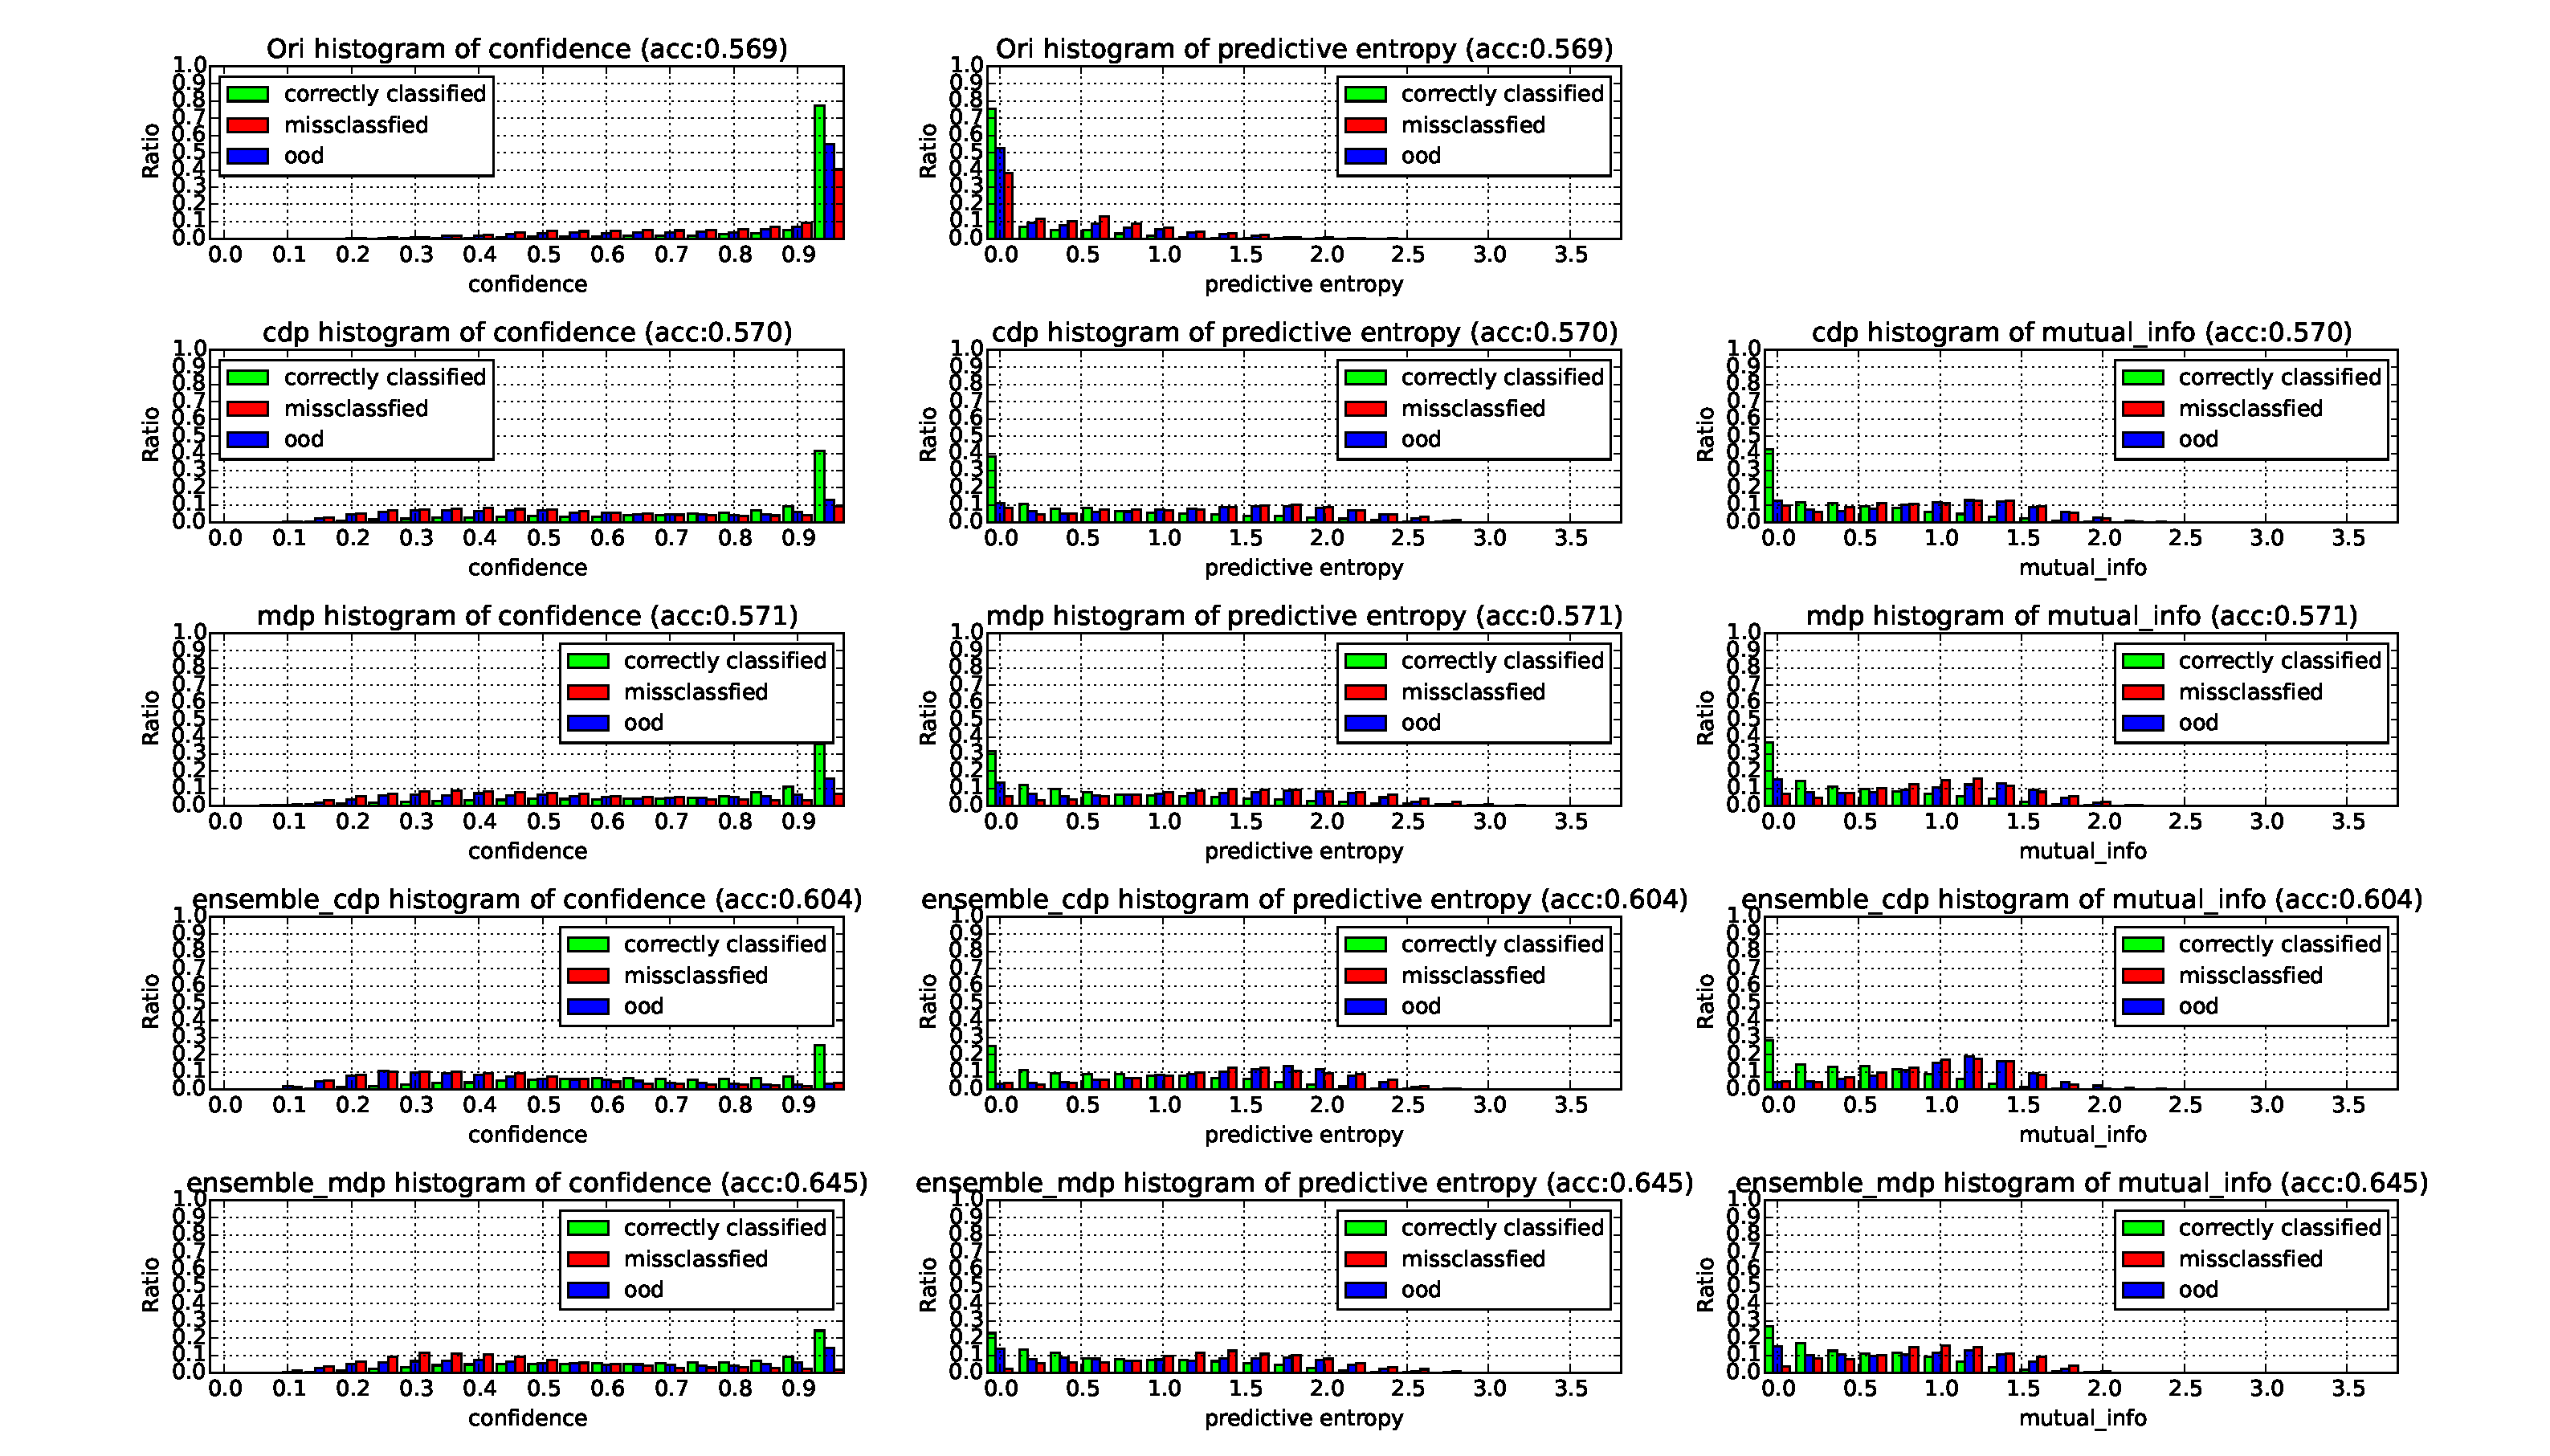
\includegraphics[height=13cm, width=16cm]{uncertainty_estimation/hist_seed3_ensemble}
		\caption{Uncertainty histograms of confidence, predictive entropy, mutual information for ori, cdp, mdp, ensemble of cdp, ensemble of mdp from one of three runs.}		
		\label{exp2_histo}
	\end{center}
\end{figure}
\begin{figure}[H]
	\begin{center}
		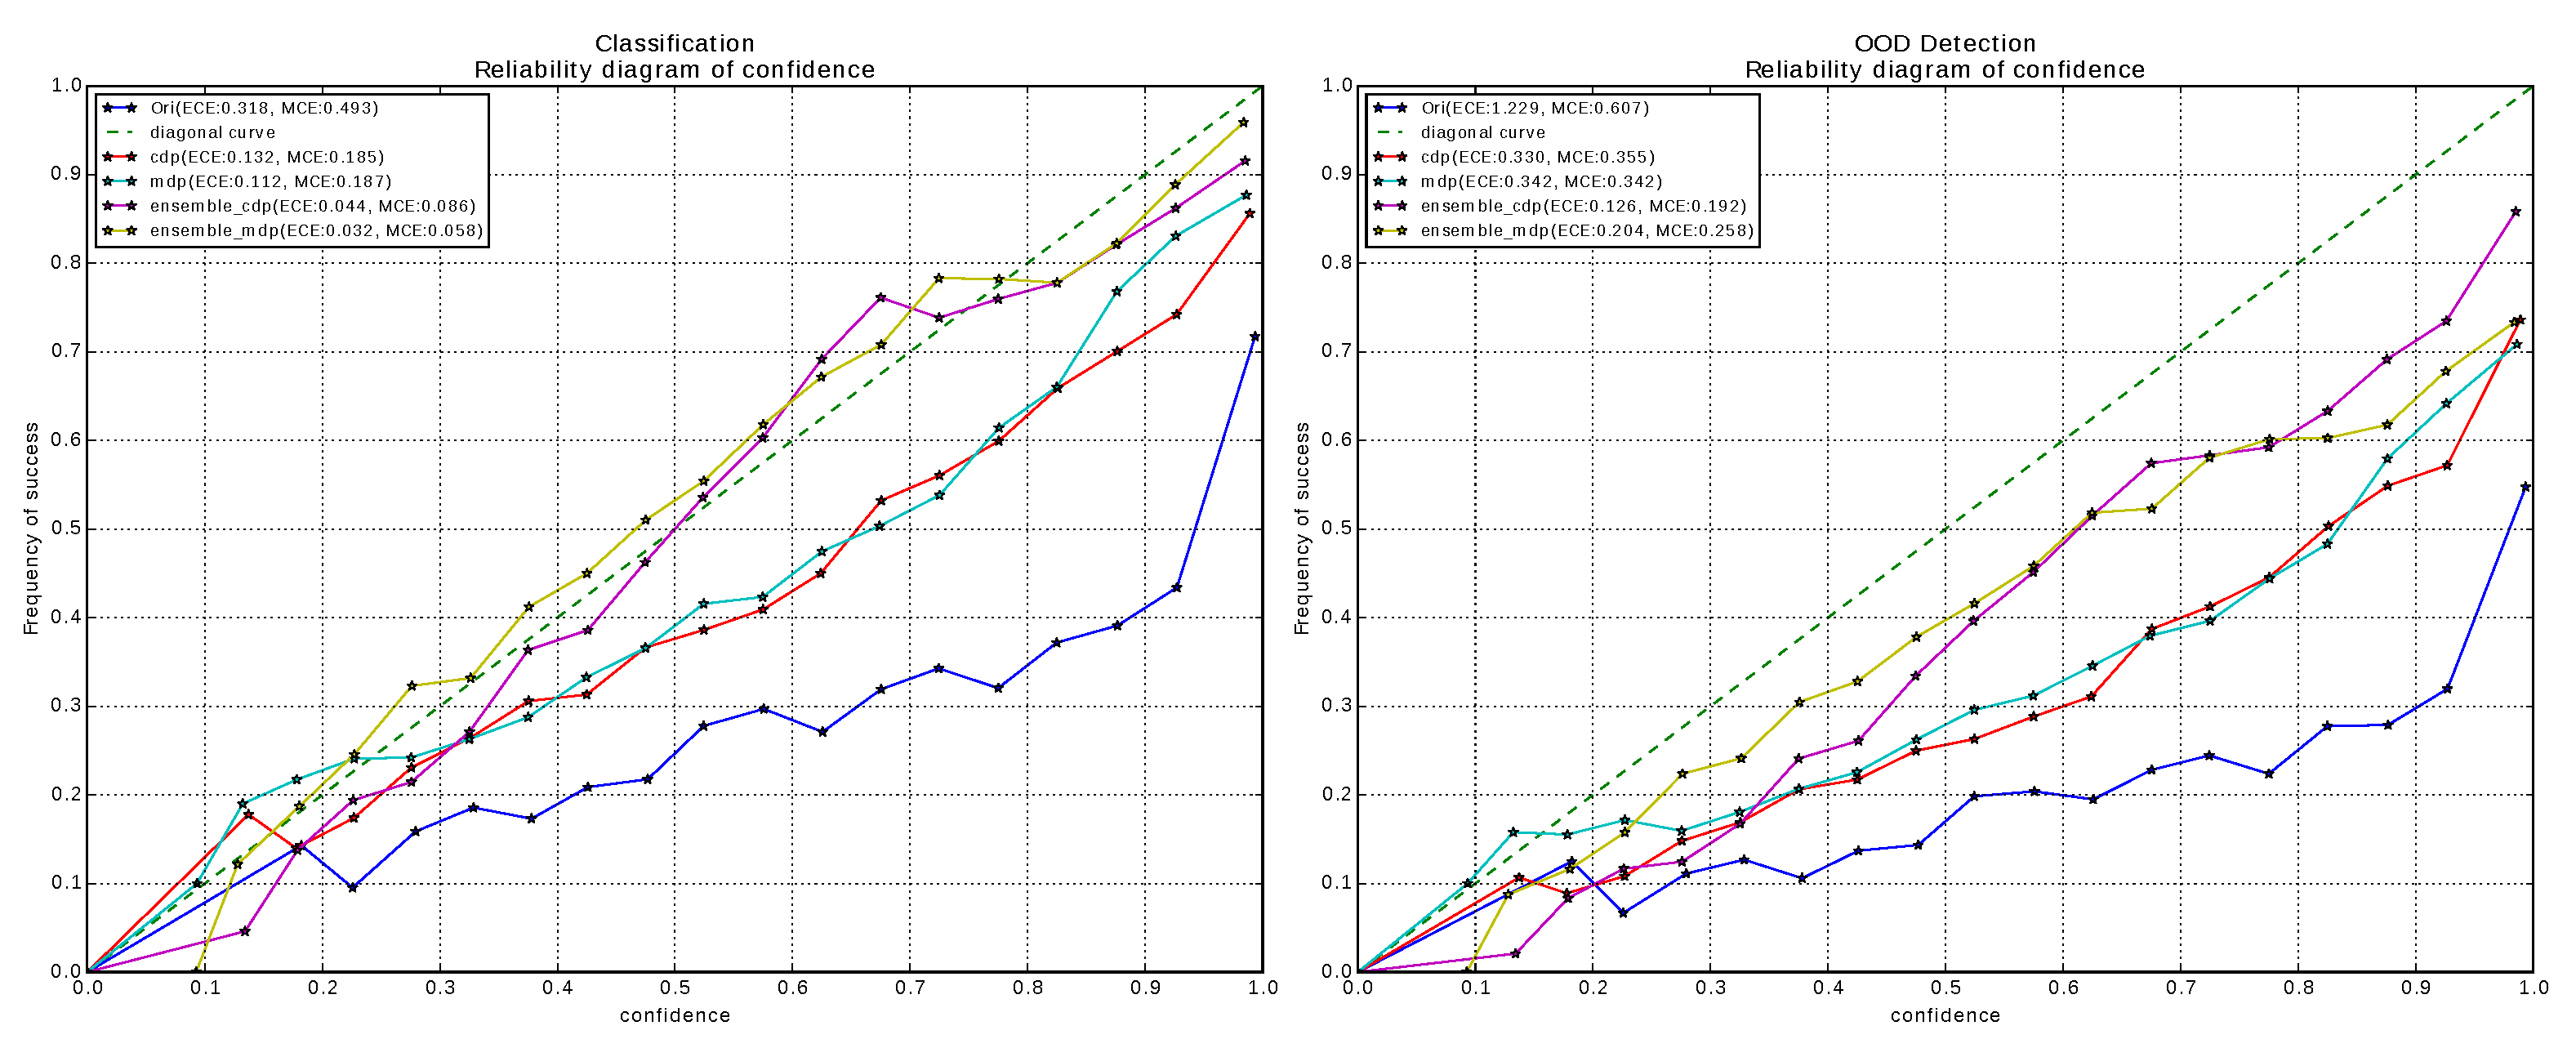
\includegraphics[height=6cm, width=16.5cm]{uncertainty_estimation/reliability_seed3_ensemble_}
		\caption{Calibration curve for ori, cdp, mdp, ensemble of cdp, ensemble of mdp from one of three runs.}		
		\label{exp2_reliability}
	\end{center}
\end{figure}

\paragraph{ROC curve and PR curve}
When it comes to the separability metrics in figure \ref{exp2_roc_pr}, as stated before, we measure separability between correct prediction and miss-classification (on the left) and that between correct prediction and OOD prediction (on the right). On separability between correction prediction and miss-classification, cdp, mdp and their ensemble version can improve the results compared with original version in both ROC curve and PR curve on the left. On the other hand, the improvements on separability between correct prediction and OOD data are more obvious on the right. However, as observed before, the ensemble of mdp does not work well with OOD data, which can be observe with this metrics. We can know more from the curves that the worse performance with OOD data in mdp is enlarged by building ensemble of it.    

\begin{figure}[h!]
	\begin{center}
		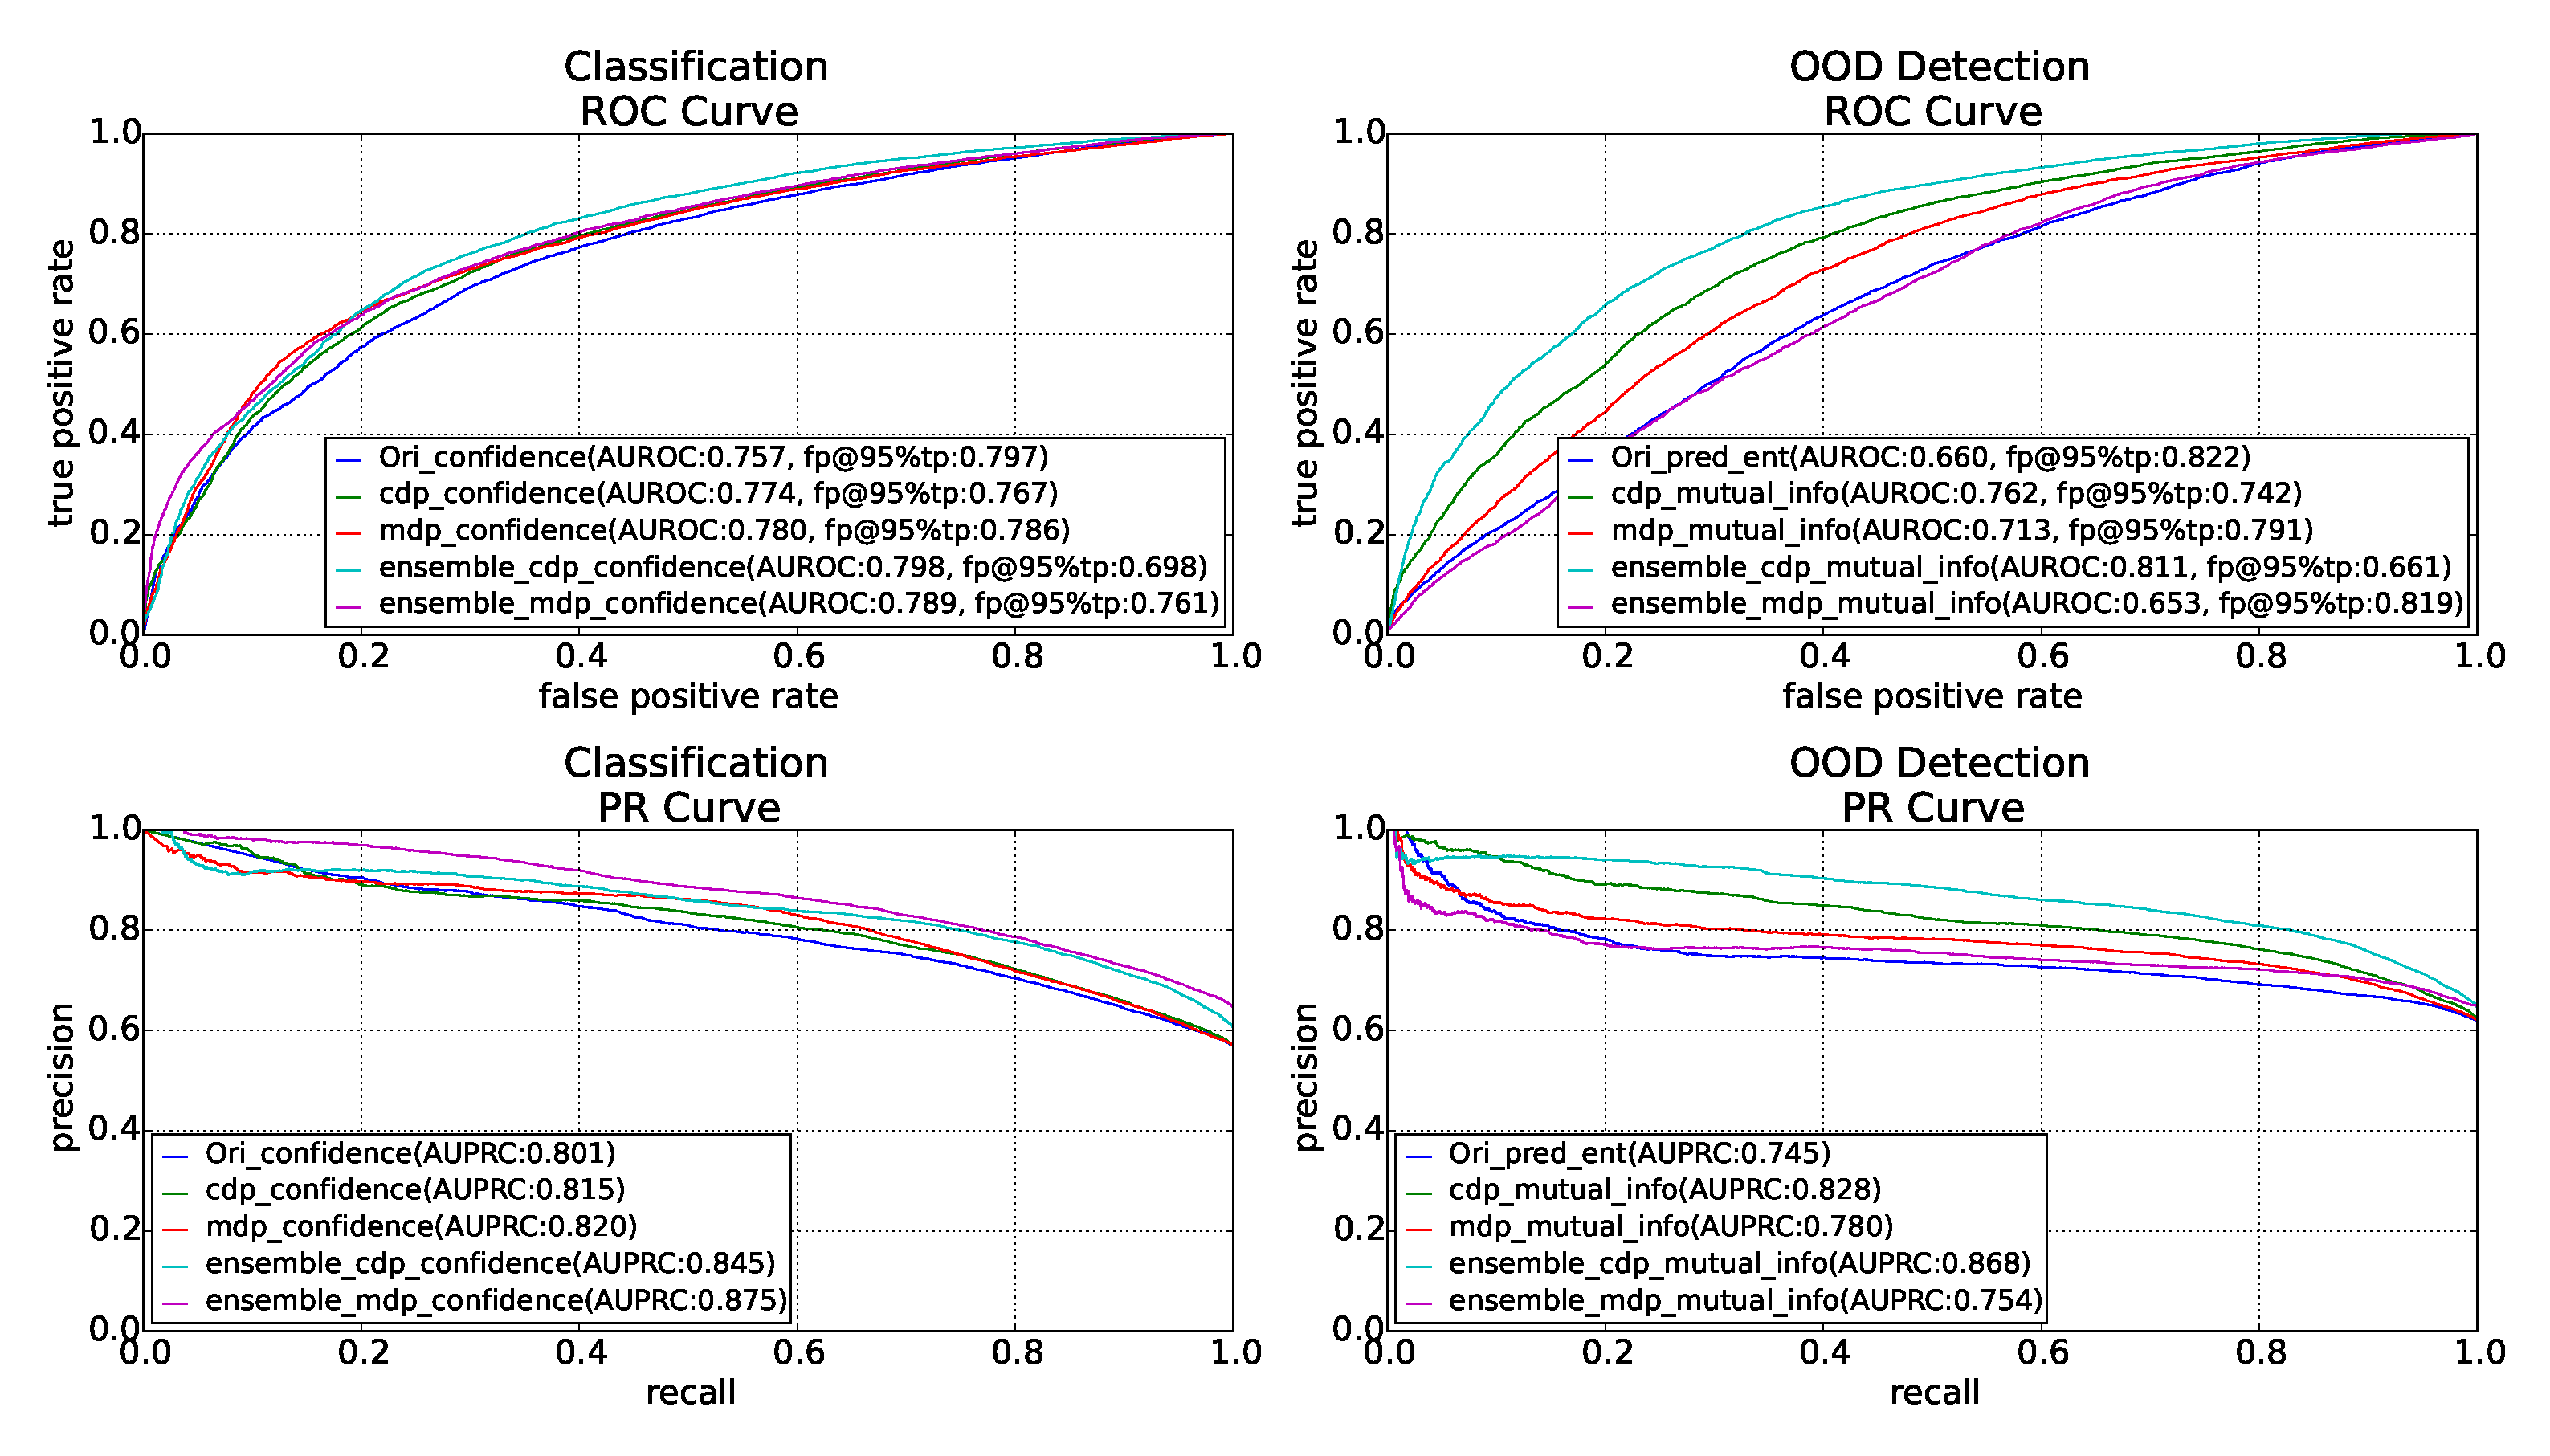
\includegraphics[height=9cm, width=16cm]{uncertainty_estimation/roc_pr_seed3_ensemble}
		\caption{ROC and PR curve of ori, cdp, mdp, ensemble of cdp, ensemble of one of three runs.}		
		\label{exp2_roc_pr}
	\end{center} 
\end{figure}

Before we only show the visual metrics for evaluation, it's better to quantify the performance quantitatively. We adopt different aforementioned metrics to achieve this which are presented in the following table \ref{table:compareWithEnsemble}. In order to exclude the influence of random initialization, we train three models of different random seeds and report the mean and standard deviation for each metric. We can see the improvements by cdp, mdp and their ensemble versions along all the metrics. The phenomenon that mdp does not work well with OOD and this effect enlarged by ensemble is also expressed in the table. Based on these experiment results, we can draw the conclusion that, concrete dropout and multiple dropout can improve both accuracy and calibration performance compared with original ResNet50. While the ensemble of concrete dropout and multiple dropout work even better without OOD data, the ensemble of multiple dropout work worse than that of concrete dropout when considering OOD data in this work. When comparing concrete dropout and multiple dropout, concrete dropout is more robust than multiple dropout because the latter one does not work well with OOD data.

\begin{table}[H]
	\centering
	\caption{Quantitative results of acc, bs, nll, ece, mce, auroc, aupr averaged from 3 different random seeds}
	\begin{tabular}{|l|l|l|l|}
		\hline
		& accuracy$ \boldsymbol\uparrow$     & brier\_score $ \boldsymbol \downarrow$& \begin{tabular}[c]{@{}l@{}}negative\\ log \\ likelihood $ \boldsymbol\downarrow$\end{tabular} \\ \hline
		ori           & 0.568$\pm$0.008 & 0.722$\pm$0.019 & 3.242$\pm$0.340                                                         \\ \hline
		cdp           & 0.577$\pm$0.008 & 0.594$\pm$0.013 & 2.088$\pm$0.181                                                         \\ \hline
		mdp           & 0.599$\pm$0.023 & 0.566$\pm$0.020 & 1.940$\pm$0.064                                                         \\ \hline
		emsemble\_cdp & 0.604        & 0.534        & 1.452                                                                \\ \hline
		emsemble\_mdp & 0.645        & 0.496        & 1.389                                                                \\ \hline
	\end{tabular}
\label{table:compareWithEnsemble}
\end{table}

\begin{table}[H]
	\centering
	% \caption{results of ece, mce, auroc, aupr}
	\begin{tabular}{|l|l|l|l|l|}
		\hline
		& \begin{tabular}[c]{@{}l@{}}expected\\ calibration\\ error(w/o. OOD/\\ w. OOD)$ \boldsymbol\downarrow$\end{tabular} & \begin{tabular}[c]{@{}l@{}}maximal\\ calibration\\ error(w/o. OOD/\\ w. OOD)$ \boldsymbol\downarrow$\end{tabular} & \begin{tabular}[c]{@{}l@{}}area under\\ ROC\\ (vs. Miss-\\ classified/\\ vs. OOD)$ \boldsymbol\uparrow$\end{tabular} & \begin{tabular}[c]{@{}l@{}}area under\\ PR curve\\ (vs. Miss-\\ classified/\\ vs. OOD)$ \boldsymbol\uparrow$\end{tabular} \\ \hline
		ori           & \begin{tabular}[c]{@{}l@{}}0.304$\pm$0.016 /\\ 0.633$\pm$0.065\end{tabular}                      & \begin{tabular}[c]{@{}l@{}}0.461$\pm$0.027 /\\ 0.362$\pm$0.025\end{tabular}                     & \begin{tabular}[c]{@{}l@{}}0.750$\pm$0.007 /\\ 0.664$\pm$0.011\end{tabular}           & \begin{tabular}[c]{@{}l@{}}0.802$\pm$0.008 /\\ 0.751$\pm$0.018\end{tabular}                \\ \hline
		cdp           & \begin{tabular}[c]{@{}l@{}}0.124$\pm$0.023/\\ 0.288$\pm$0.048\end{tabular}                         & \begin{tabular}[c]{@{}l@{}}0.206$\pm$0.015/ \\ 0.374$\pm$0.018\end{tabular}                     & \begin{tabular}[c]{@{}l@{}}0.775$\pm$0.008/ \\ 0.783$\pm$0.022\end{tabular}           & \begin{tabular}[c]{@{}l@{}}0.825$\pm$0.007/ \\ 0.850$\pm$0.022\end{tabular}                \\ \hline
		mdp           & \begin{tabular}[c]{@{}l@{}}0.114$\pm$0.012/ \\ 0.383$\pm$0.046\end{tabular}                      & \begin{tabular}[c]{@{}l@{}}0.199$\pm$0.016/ \\ 0.367$\pm$0.023\end{tabular}                     & \begin{tabular}[c]{@{}l@{}}0.780$\pm$0.011/ \\ 0.709$\pm$0.004\end{tabular}           & \begin{tabular}[c]{@{}l@{}}0.838$\pm$0.013/ \\ 0.788$\pm$0.006\end{tabular}                \\ \hline
		emsemble\_cdp & \begin{tabular}[c]{@{}l@{}}0.044/\\0.042 \end{tabular} 
		 &  \begin{tabular}[c]{@{}l@{}}0.086/\\0.093 \end{tabular}                                                                                    & \begin{tabular}[c]{@{}l@{}}0.798/\\0.811  \end{tabular}                                                                           & \begin{tabular}[c]{@{}l@{}}0.845/\\0.868  \end{tabular}                                                                                \\ \hline
		emsemble\_mdp & \begin{tabular}[c]{@{}l@{}}0.032/\\0.170 \end{tabular}                                                                                       & \begin{tabular}[c]{@{}l@{}}0.058/\\0.227  \end{tabular}                                                                                     & \begin{tabular}[c]{@{}l@{}}0.789/\\0.653 \end{tabular}                                                                            & \begin{tabular}[c]{@{}l@{}}0.875/\\0.754  \end{tabular}                                                                                \\ \hline
	\end{tabular}
\end{table}	

\newpage
\subsubsection{Comparison with Laplace approximation}
Because Laplace approximation requires only MAP point estimate of model parameter. Therefore we take the already trained model of different approaches as our MAP point estimate and compute the approximation of Kronecker factors with half of training set. We set the scale parameter of Kronecker factors $\sqrt{N}$ as $1$ and dump factor $\sqrt{\tau}$ as $15$ in equation \ref{mvg_prior} based on grid search on the validation set.   

In the following figures, we show the histograms, calibration curves, ROC curve and PR curve of cdp, mdp and their Laplace approximation versions. We can see that the Laplace approximation can achieve similar results as the cdp or mdp do in uncertainty histograms, calibration curves as well as ROC curve and PR curve. The histograms of different uncertainty measure show similar trend as before. 

If we compare the Laplace approximation between cdp and mdp, we can see that the result of Laplace approximation is similar to the their dropout versions. This can be observed through that the percentage of OOD prediction with high confidence of Laplace approximation for network trained with mdp is higher than that of Laplace approximation for network trained with cdp in the histogram. Besides, in ROC curve/PR curve on correct prediction vs. OOD data prediction of mdp and cdp, the area under curve of Laplace approximation of mdp is obviously lower than that of cdp. This phenomenon also exists in the histogram and ROC as well as PR curve of mdp and cdp. In the table of quantitative results (cf. \ref{table:lap}), the quantities of different metrics corresponding to the visual metrics. To summarize this, although Laplace can achieve similar results as concrete dropout and multiple dropout do, their performance is highly related to the point estimate of parameter obtained during training.

\begin{figure}[H]
	\begin{center}
		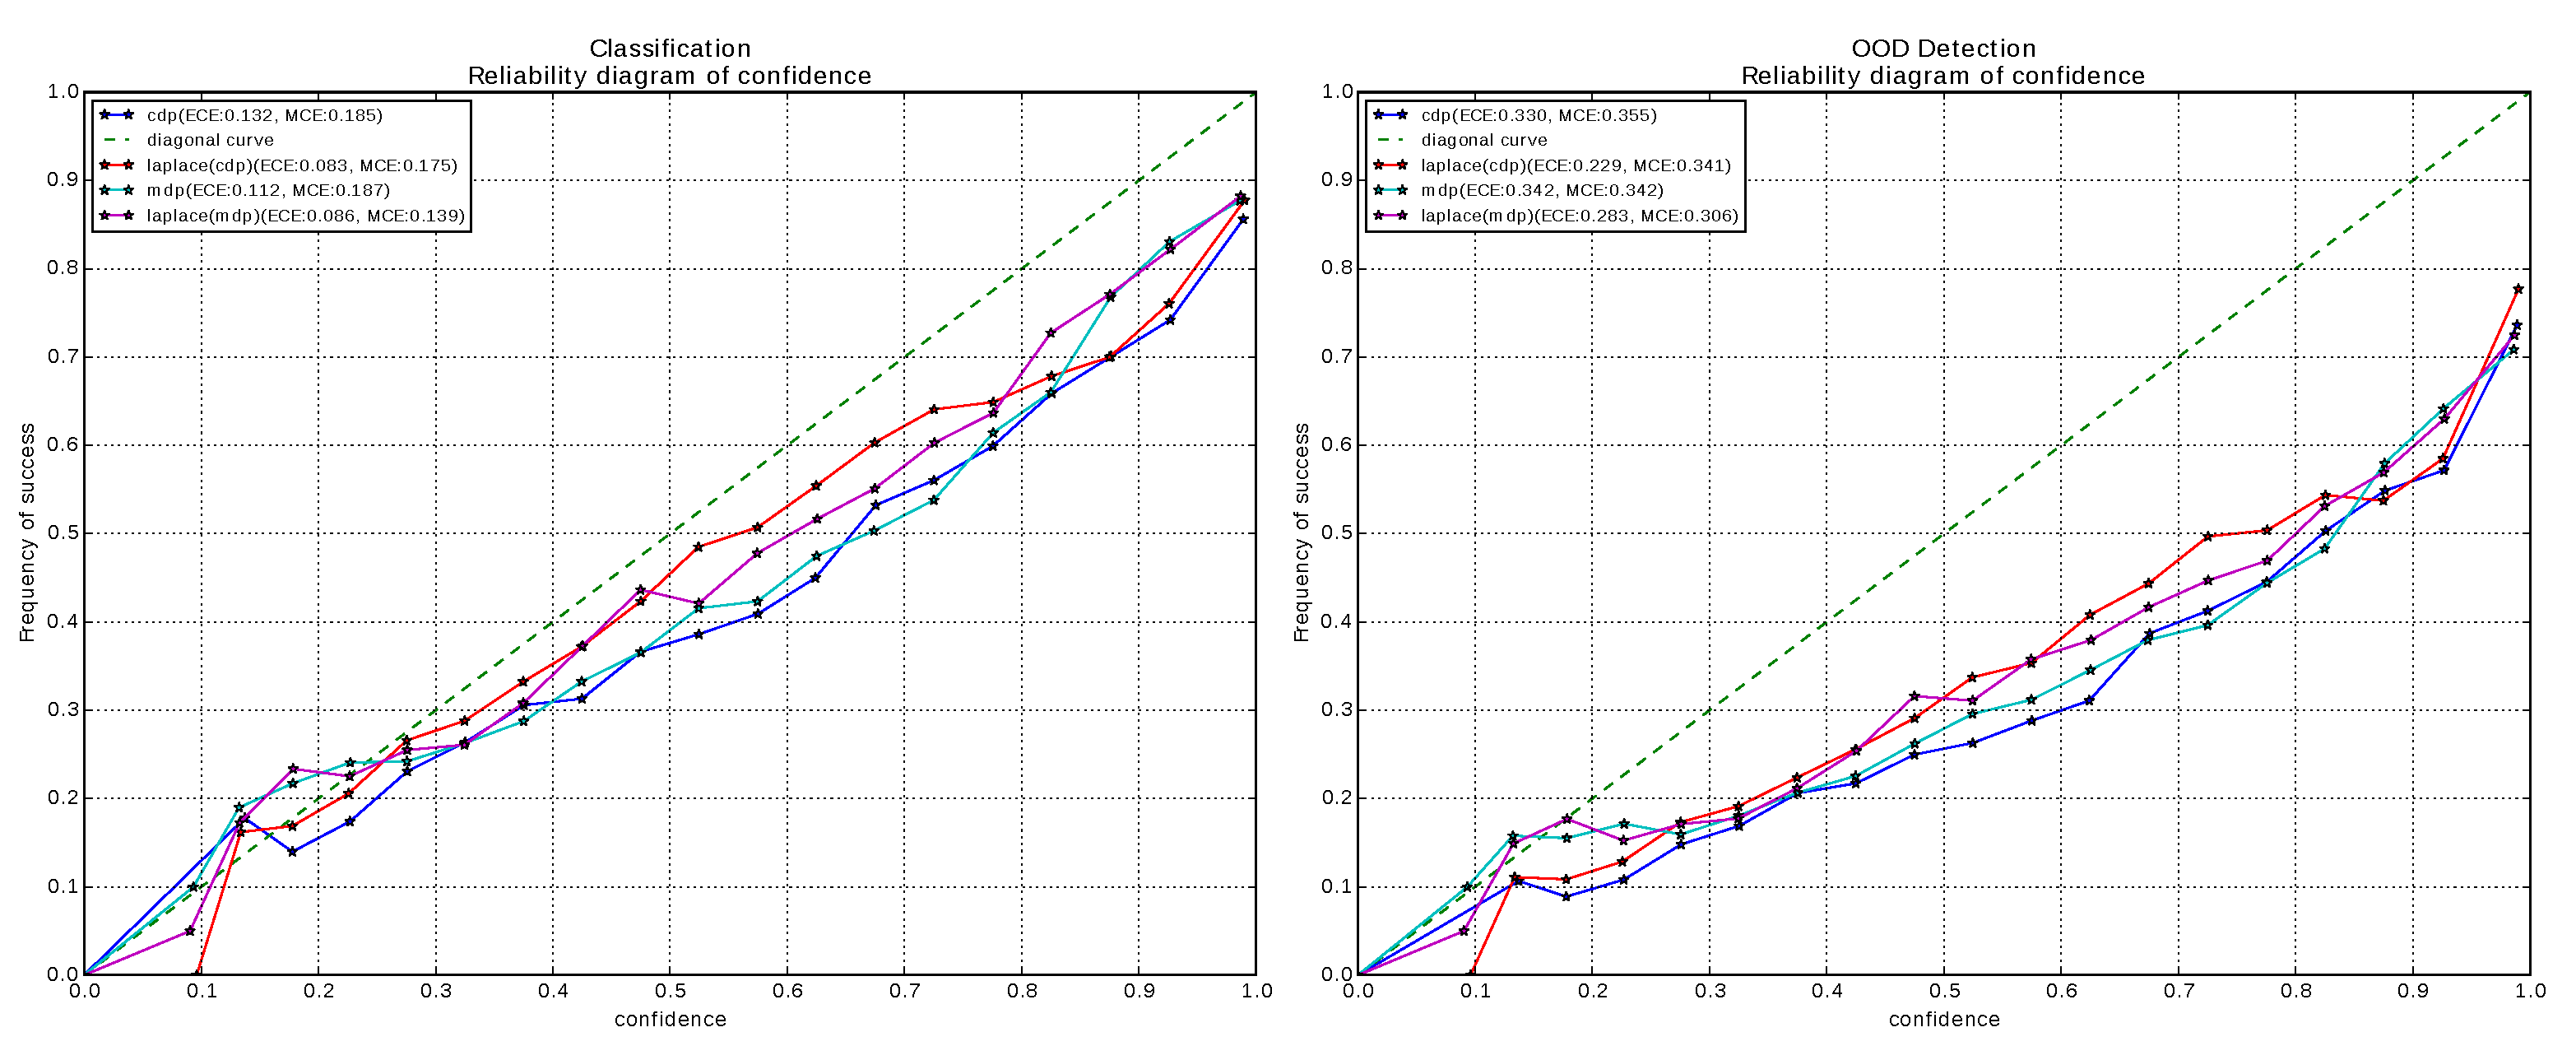
\includegraphics[height=5cm, width=16.5cm]{uncertainty_estimation/laplace/reliabilty_seed3_}
		\caption{Calibration curve of cdp, mdp and their Laplace approximation versions from one of three runs.}		
		\label{lap_calibration}
	\end{center}
\end{figure}

\begin{figure}[h!]		
	\centering
	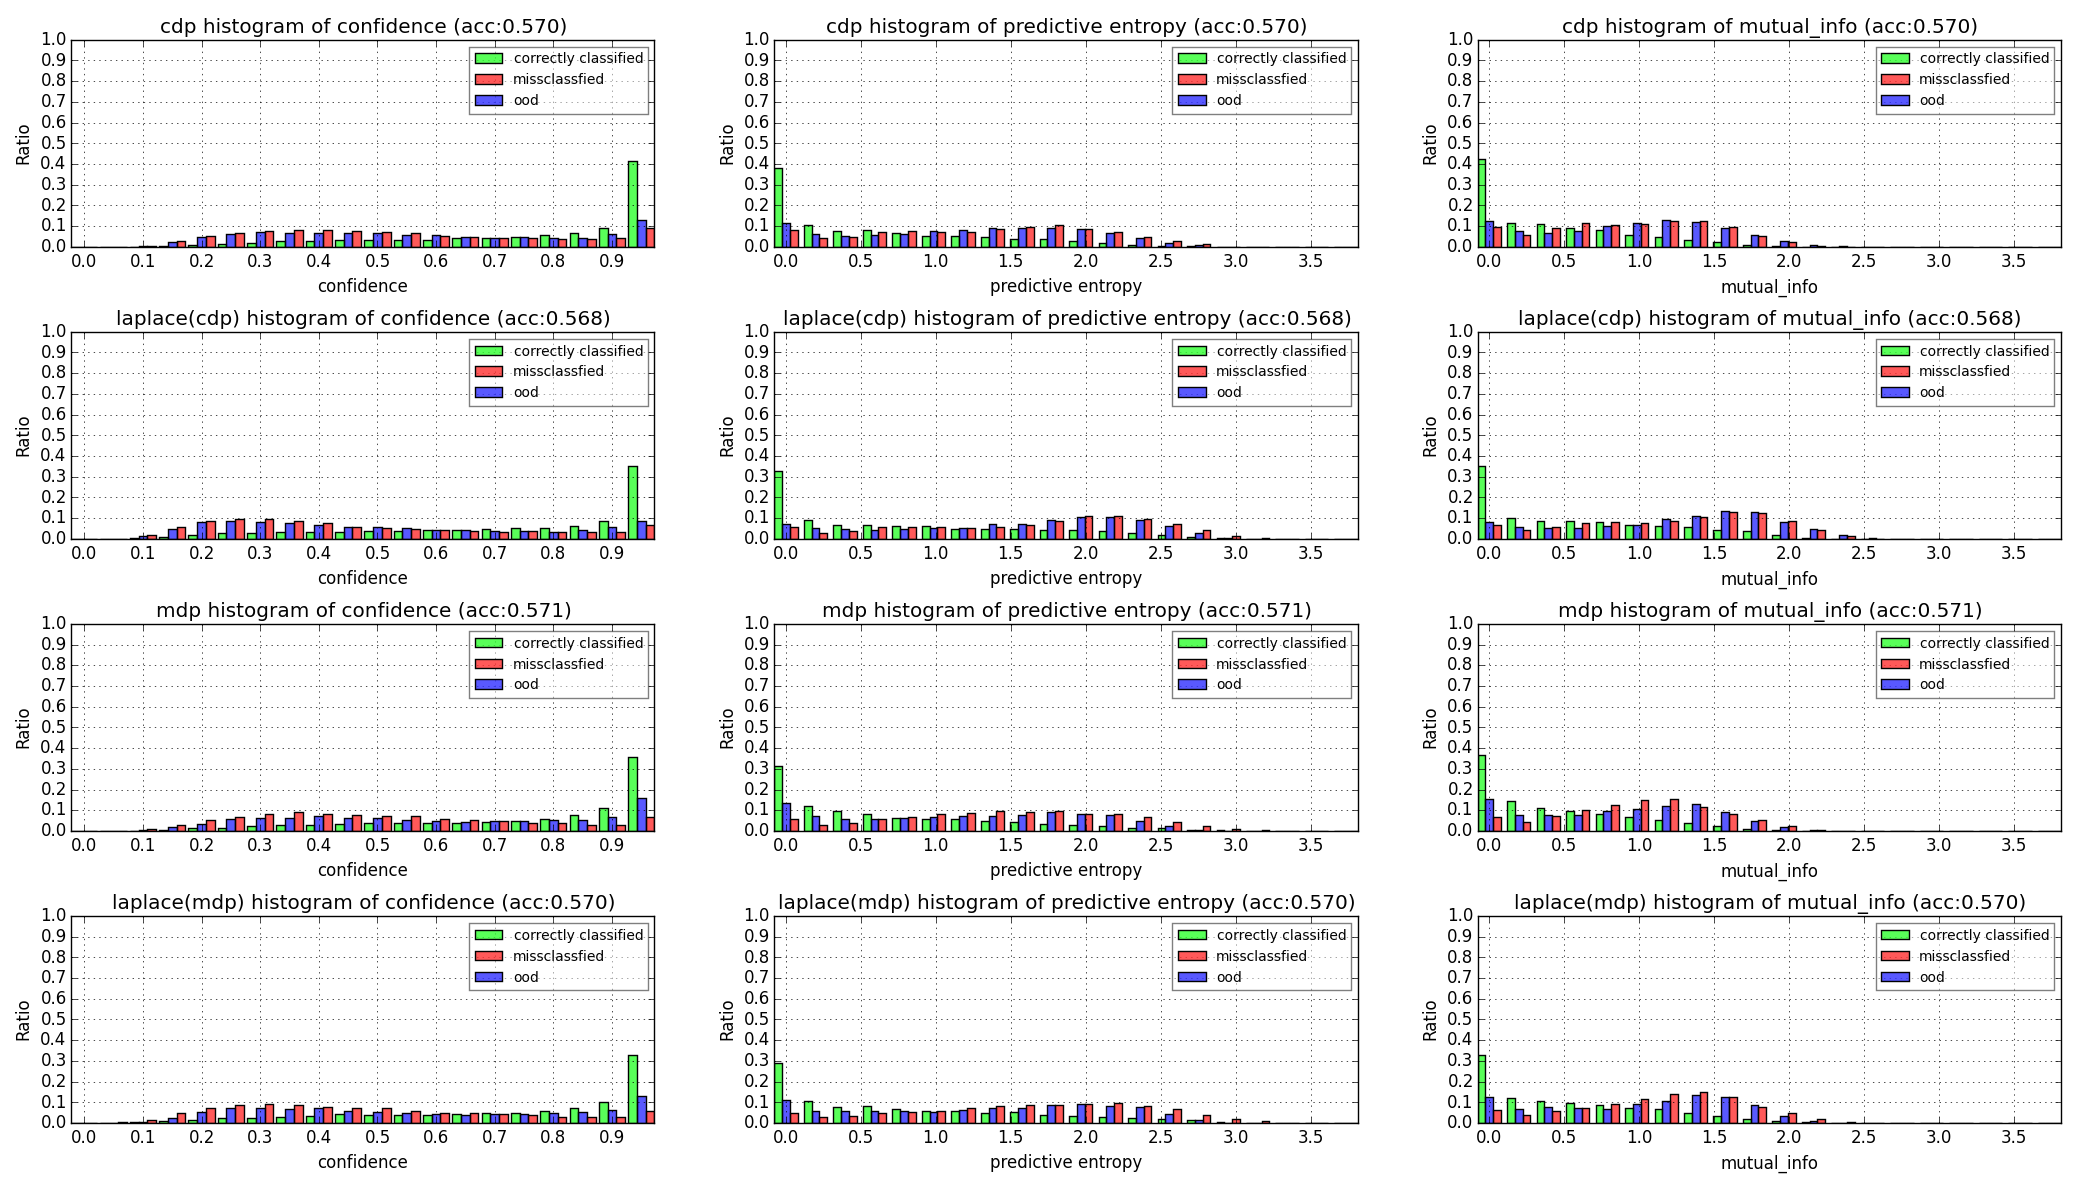
\includegraphics[height=10cm, width=16cm]{uncertainty_estimation/laplace/histo_ood_seed3}
	\caption{Uncertainty histogram of cdp, mdp and their Laplace approximation versions with confidence, predictive entropy and mutual information as uncertainty measure in one of three runs.}
	\label{figure:lap_hist}	
\end{figure}


\begin{figure}[H]
	\begin{center}
		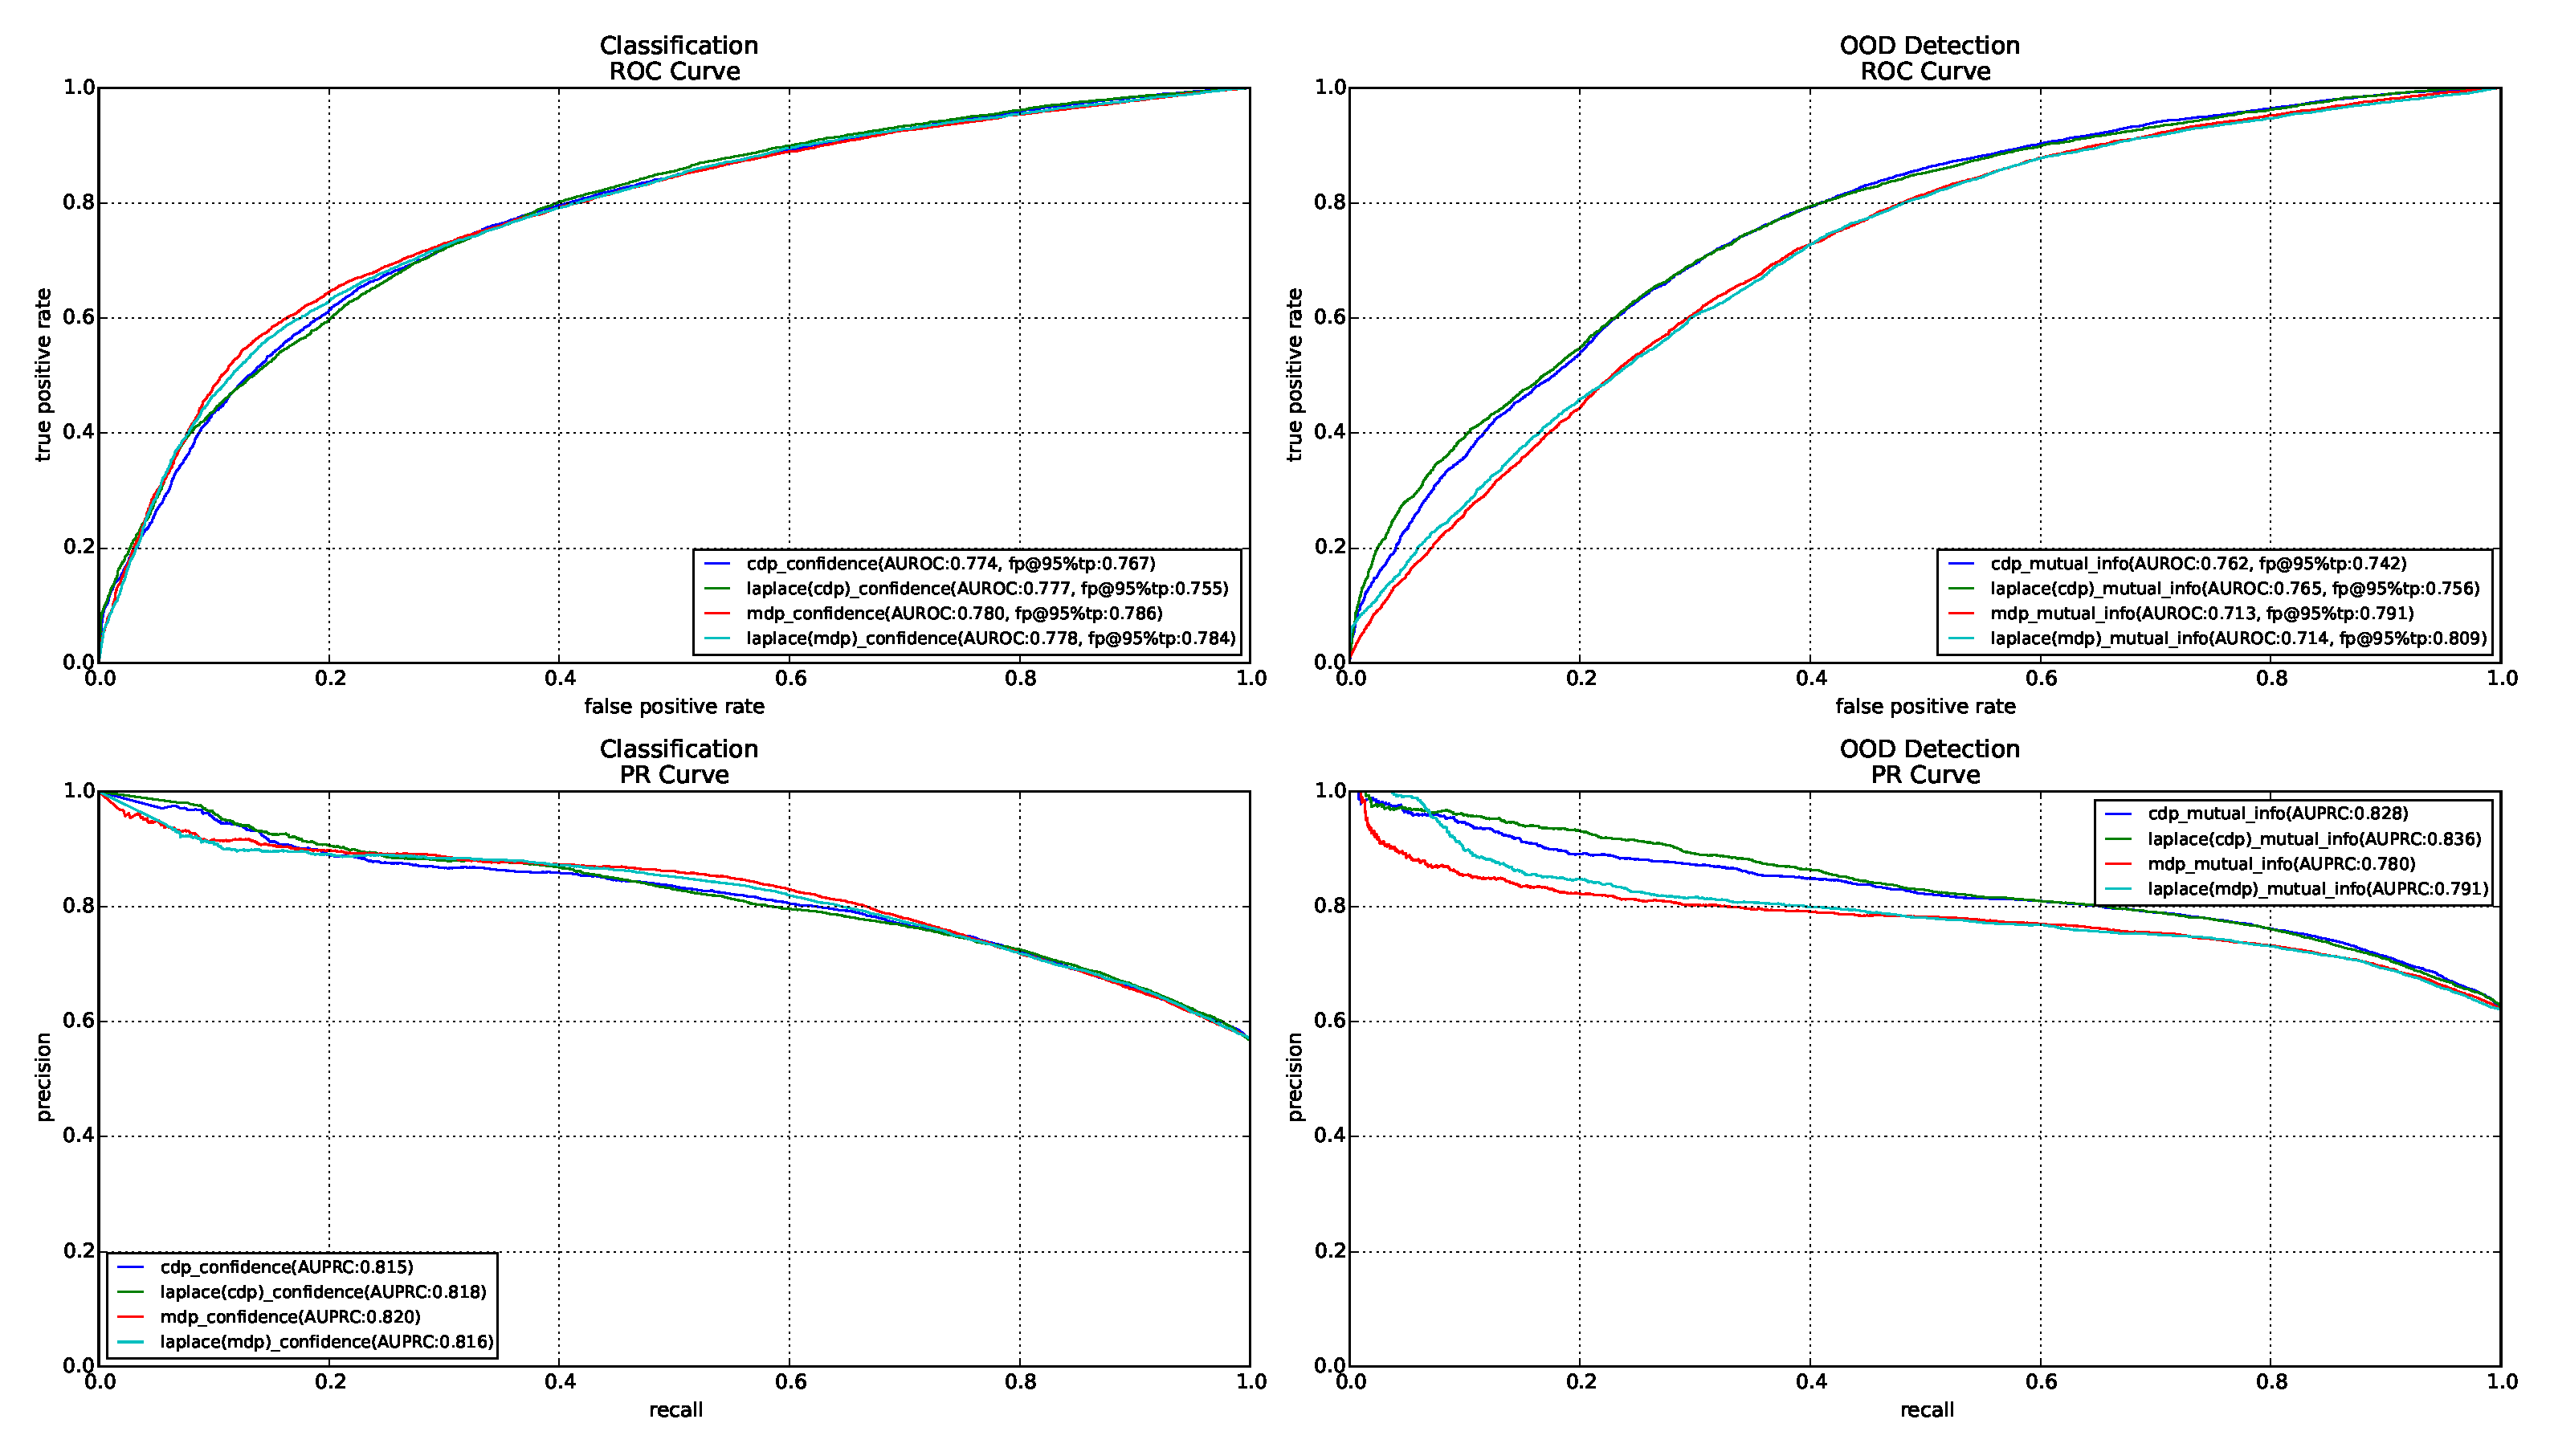
\includegraphics[height=9cm, width=16cm]{uncertainty_estimation/laplace/roc_pr_seed3}
		\caption{ROC and PR curve of cdp, mdp and their Laplace approximation versions from one of three runs.}		
		\label{lap_roc_pr}
	\end{center}
\end{figure}

\begin{table}[H]
	\centering
	\label{table:lap}
	\caption{Quantitative results of acc, bs, nll, ece, mce, auroc, aupr averaged from 3 different random seeds}
	\begin{tabular}{|l|l|l|l|}
		\hline
		& accuracy  $\boldsymbol \uparrow$                                                            & brier score $\boldsymbol \downarrow$                                                           & \begin{tabular}[c]{@{}l@{}}negative \\ log\\ likelihood $\boldsymbol \downarrow$\end{tabular}  \\ \hline
		cdp          & 
		\begin{tabular}[c]{@{}l@{}}0.577$\pm$0.008\end{tabular} & 
		\begin{tabular}[c]{@{}l@{}}0.594$\pm$0.013\end{tabular} & \begin{tabular}[c]{@{}l@{}}2.088$\pm$0.181\end{tabular} \\ \hline
		
		laplace\_cdp & 
		\begin{tabular}[c]{@{}l@{}}0.576$\pm$0.009\end{tabular}    & \begin{tabular}[c]{@{}l@{}}0.602$\pm$0.011\end{tabular} & \begin{tabular}[c]{@{}l@{}}2.322$\pm$0.350\end{tabular} \\ \hline
		
		mdp          & 
		\begin{tabular}[c]{@{}l@{}}0.599$\pm$0.023\end{tabular} & \begin{tabular}[c]{@{}l@{}}0.566$\pm$0.020\end{tabular} & \begin{tabular}[c]{@{}l@{}}1.940$\pm$0.064\end{tabular} \\ \hline
		laplace\_mdp & 		\begin{tabular}[c]{@{}l@{}}0.598$\pm$0.024\end{tabular} & \begin{tabular}[c]{@{}l@{}}0.567$\pm$0.018\end{tabular} & \begin{tabular}[c]{@{}l@{}}1.970$\pm$0.117\end{tabular} \\ \hline
	\end{tabular}
\end{table}
\begin{table}[H]
	\centering
	\begin{tabular}{|l|l|l|l|l|}
		\hline
		& \begin{tabular}[c]{@{}l@{}}expected\\ calibration\\ error(w/o. OOD/\\ w. OOD) $\boldsymbol \downarrow$\end{tabular} & \begin{tabular}[c]{@{}l@{}}maximal\\ calibration\\ error(w/o. OOD/\\ w. OOD)$\boldsymbol \downarrow$\end{tabular} & \begin{tabular}[c]{@{}l@{}}area under\\ ROC\\ (vs. Miss-\\ classified/\\ vs. OOD)$\boldsymbol \uparrow$\end{tabular} & \begin{tabular}[c]{@{}l@{}}area under\\ PR curve\\ (vs. Miss-\\ classified/\\ vs. OOD)$\boldsymbol \uparrow$\end{tabular} \\ \hline
		
		cdp          & \begin{tabular}[c]{@{}l@{}}0.124$\pm$0.023/ \\0.288$\pm$0.048\end{tabular}                      & \begin{tabular}[c]{@{}l@{}}0.206$\pm$0.015/ \\0.374$\pm$0.018\end{tabular}                     & \begin{tabular}[c]{@{}l@{}}0.775$\pm$0.008/ \\0.783$\pm$0.022\end{tabular}           & \begin{tabular}[c]{@{}l@{}}0.825$\pm$0.007/ \\0.850$\pm$0.022\end{tabular}                \\ \hline
		
		laplace\_cdp & \begin{tabular}[c]{@{}l@{}}0.129$\pm$0.058/ \\0.341$\pm$0.157\end{tabular}                         & \begin{tabular}[c]{@{}l@{}}0.235$\pm$0.073/ \\0.406$\pm$0.070\end{tabular}                     & \begin{tabular}[c]{@{}l@{}}0.779$\pm$0.004/ \\0.782$\pm$0.017\end{tabular}           & \begin{tabular}[c]{@{}l@{}}0.826$\pm$0.007/ \\0.849$\pm$0.016\end{tabular}                \\ \hline
		
		mdp          & \begin{tabular}[c]{@{}l@{}}0.114$\pm$0.012/ \\0.383$\pm$0.046\end{tabular}                      & \begin{tabular}[c]{@{}l@{}}0.199$\pm$0.016/ \\0.367$\pm$0.023\end{tabular}                     & \begin{tabular}[c]{@{}l@{}}0.780$\pm$0.011/ \\0.709$\pm$0.004\end{tabular}           & \begin{tabular}[c]{@{}l@{}}0.838$\pm$0.013/ \\0.788$\pm$0.006\end{tabular}                \\ \hline
		
		laplace\_mdp         & \begin{tabular}[c]{@{}l@{}} 0.104$\pm$0.018/ \\0.352$\pm$0.061\end{tabular}                      & \begin{tabular}[c]{@{}l@{}}0.179$\pm$0.029/ \\0.352$\pm$0.038\end{tabular}                     & \begin{tabular}[c]{@{}l@{}}0.776$\pm$0.012/ \\0.711$\pm$0.005\end{tabular}           & \begin{tabular}[c]{@{}l@{}}0.837$\pm$0.015/ \\0.798$\pm$0.005\end{tabular}                \\ \hline
	\end{tabular}
\end{table}
\subsubsection{Ablation study}
As we can see from the previous results, mdp can work better than cdp without considering OOD data. However, it underperforms when OOD data is included. In order to investigate the reason behind this, we have done a ablation study to check the influence of aleatoric uncertainty which comes from mainly the feature extractor part. Considering this, we freeze the parameters of feature extractor and just train our probabilistic classifier which is a three-layer MLP. In the following we show the results of this ablation study with the same metrics used before. It's clear that the accuracy would drop when the feature extractor is frozen. However, we can see that mdp can have better  calibration performance than cdp and much better than original ResNet50. Regarding the separability metrics, although mdp still doesn't work better than cdp, the gap between is much smaller than the version without freezing feature extractor. These observations are expressed quantitatively in the table \ref{ab_table}. 

Based on these observations, we know that the underperformance of mdp on OOD dataset can attribute to the influence of aleatoric uncertainty. If the feature extractor is not frozen, then the aleatoric uncertainty is trained to adapt to the dataset. The problem why optimizing dropout rates for each hidden units can change the point estimate of the model parameter to have low aleatoric uncertainty for OOD data arises now. One possible reason for this could be the variance of estimation of derivatives of variational parameters is too large because of increased number of variational parameters\cite{kingma2015variational}. And the larger variances are back propagated to the feature extractor which may make the point estimate deviate from the better local minimum. One possible solution to resolve this is to sample the realization of activations of hidden units independent to each data instance, which may decrease the variance and help to improve the results. 

\begin{figure}[H]
	\begin{center}
		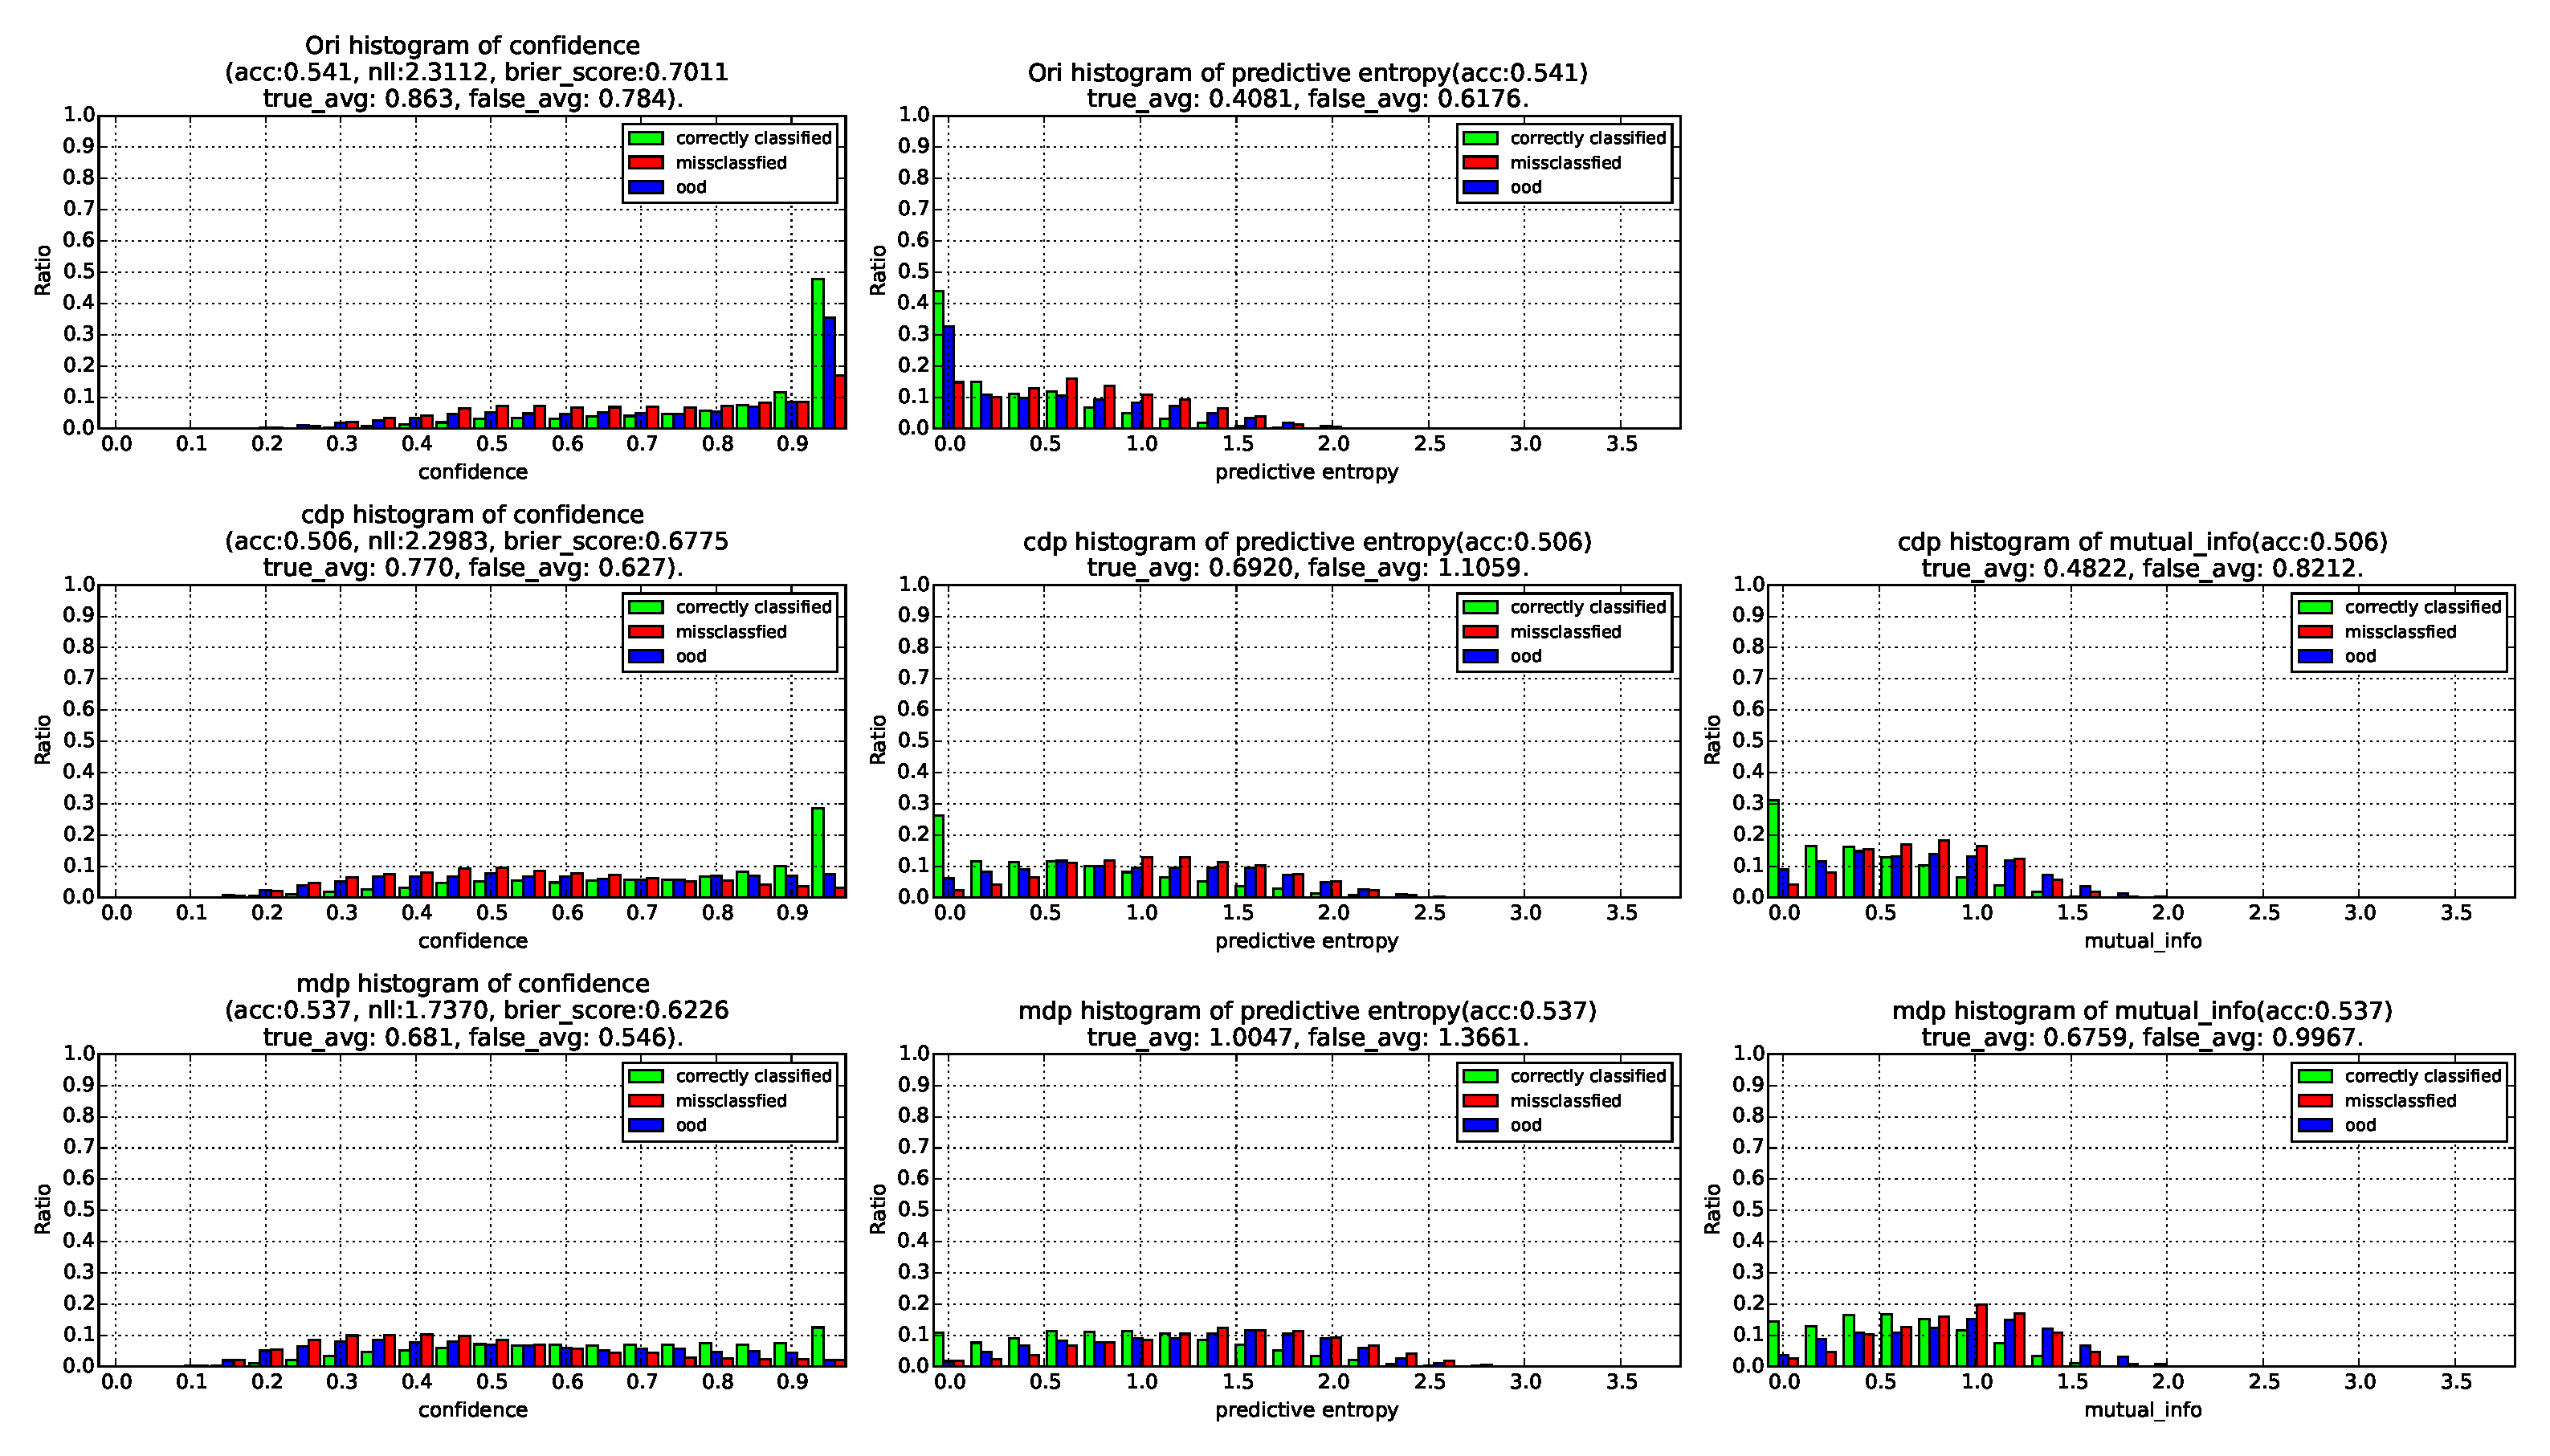
\includegraphics[height=9cm, width=16cm]{uncertainty_estimation/ablation_study/histo_froFeat_ori_cdp_mdp_ood_seed3.eps}
		\caption{Uncertainty histogram of one of three runs.}		
		\label{ab_reliability}
	\end{center}
\end{figure}

\begin{figure}[H]
	\begin{center}
		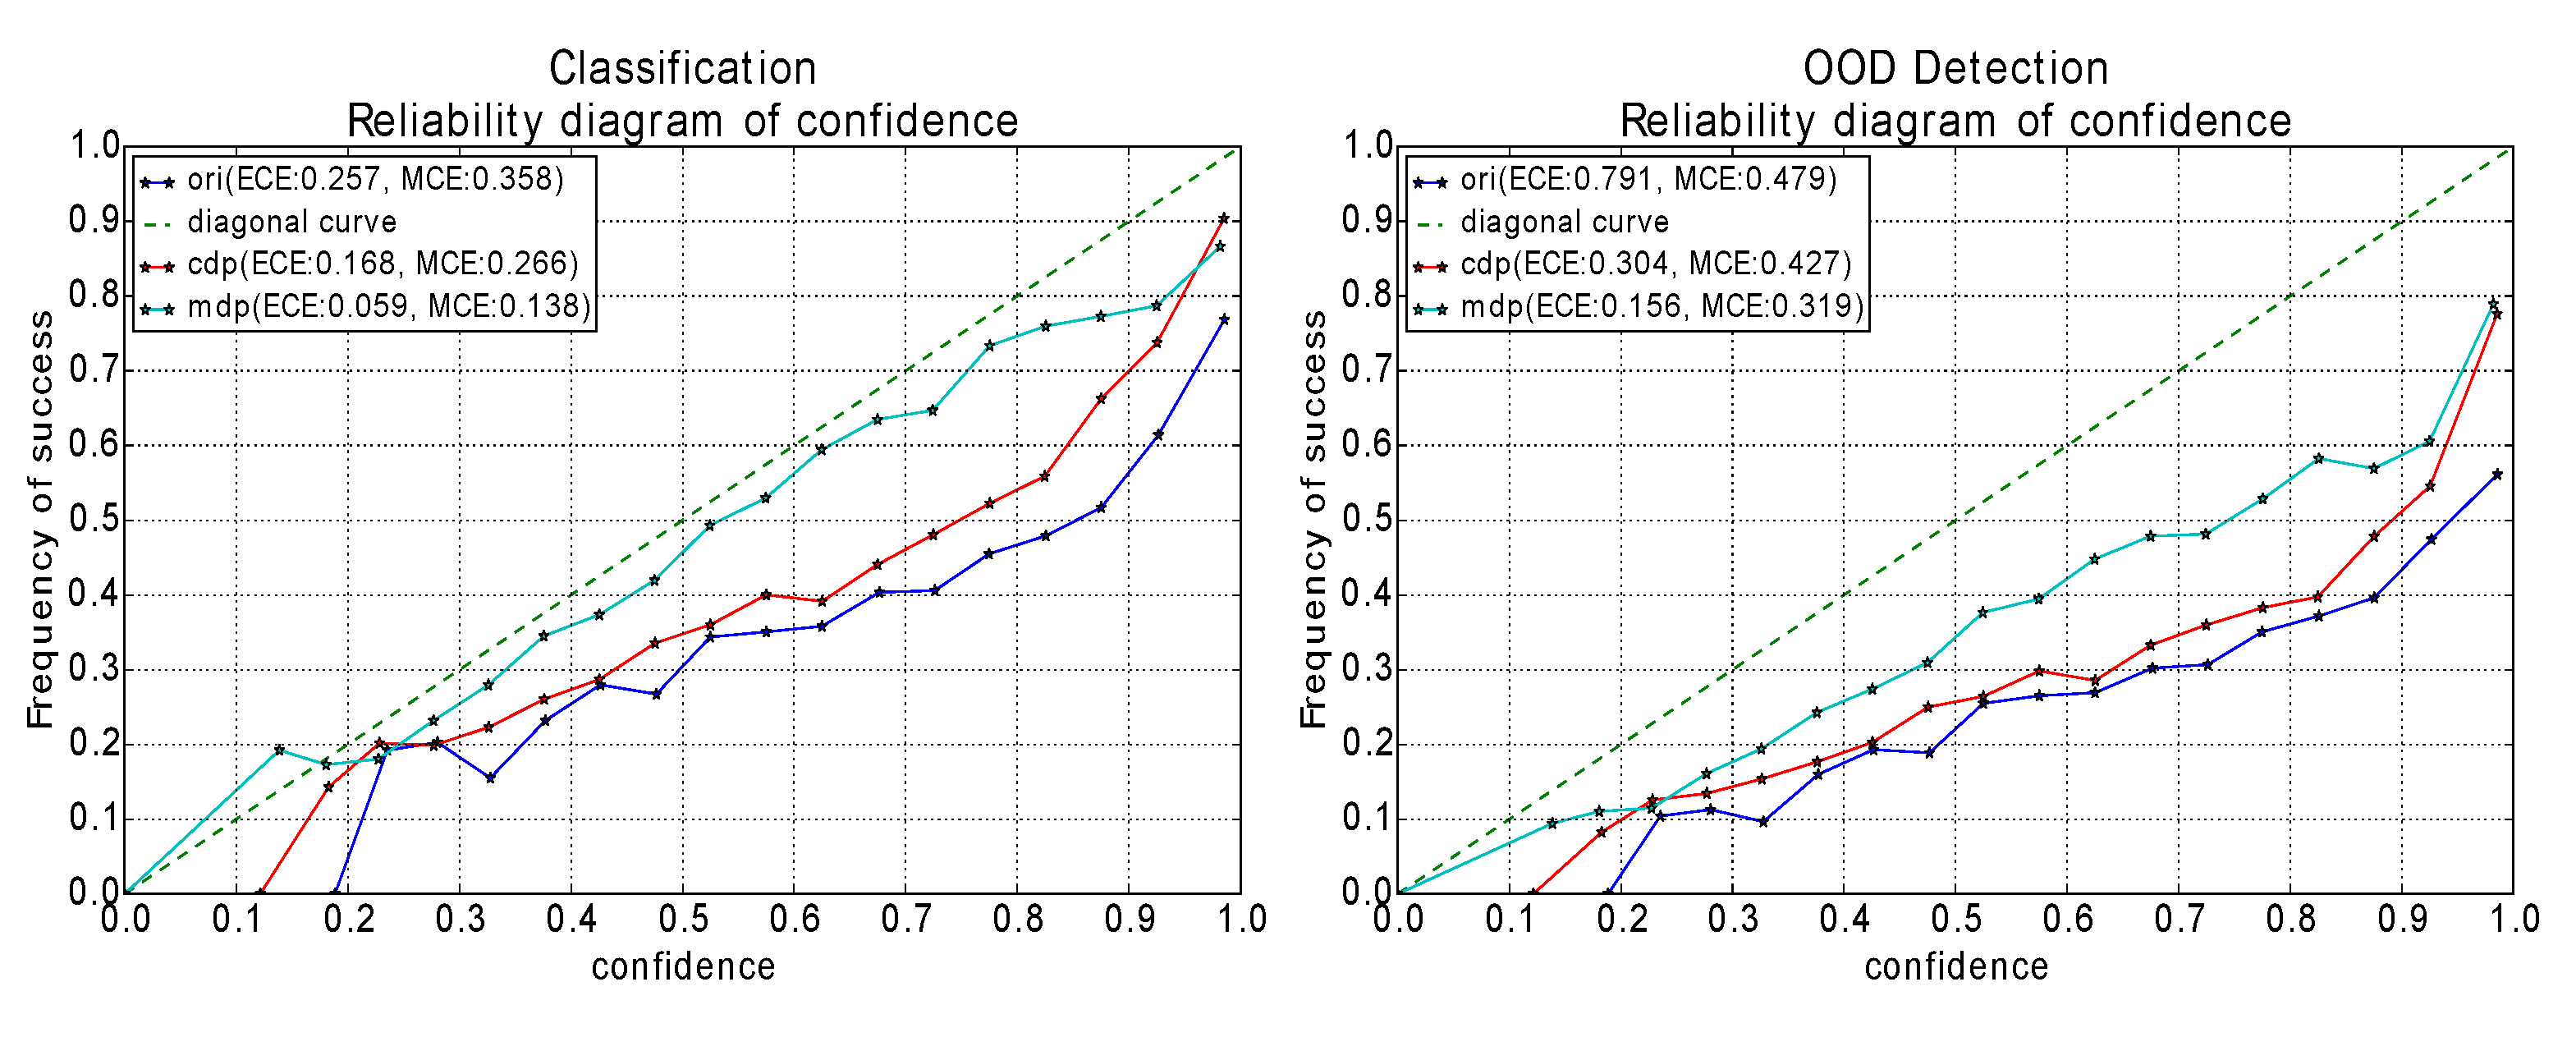
\includegraphics[height=5cm, width=16.5cm]{uncertainty_estimation/ablation_study/reliability_froFeat_ori_cdp_mdp_combined_seed3_.eps}
		\caption{Calibration curve of one of three runs.}		
		\label{ab_calibration}
	\end{center}
\end{figure}


\begin{figure}[H]
	\begin{center}
		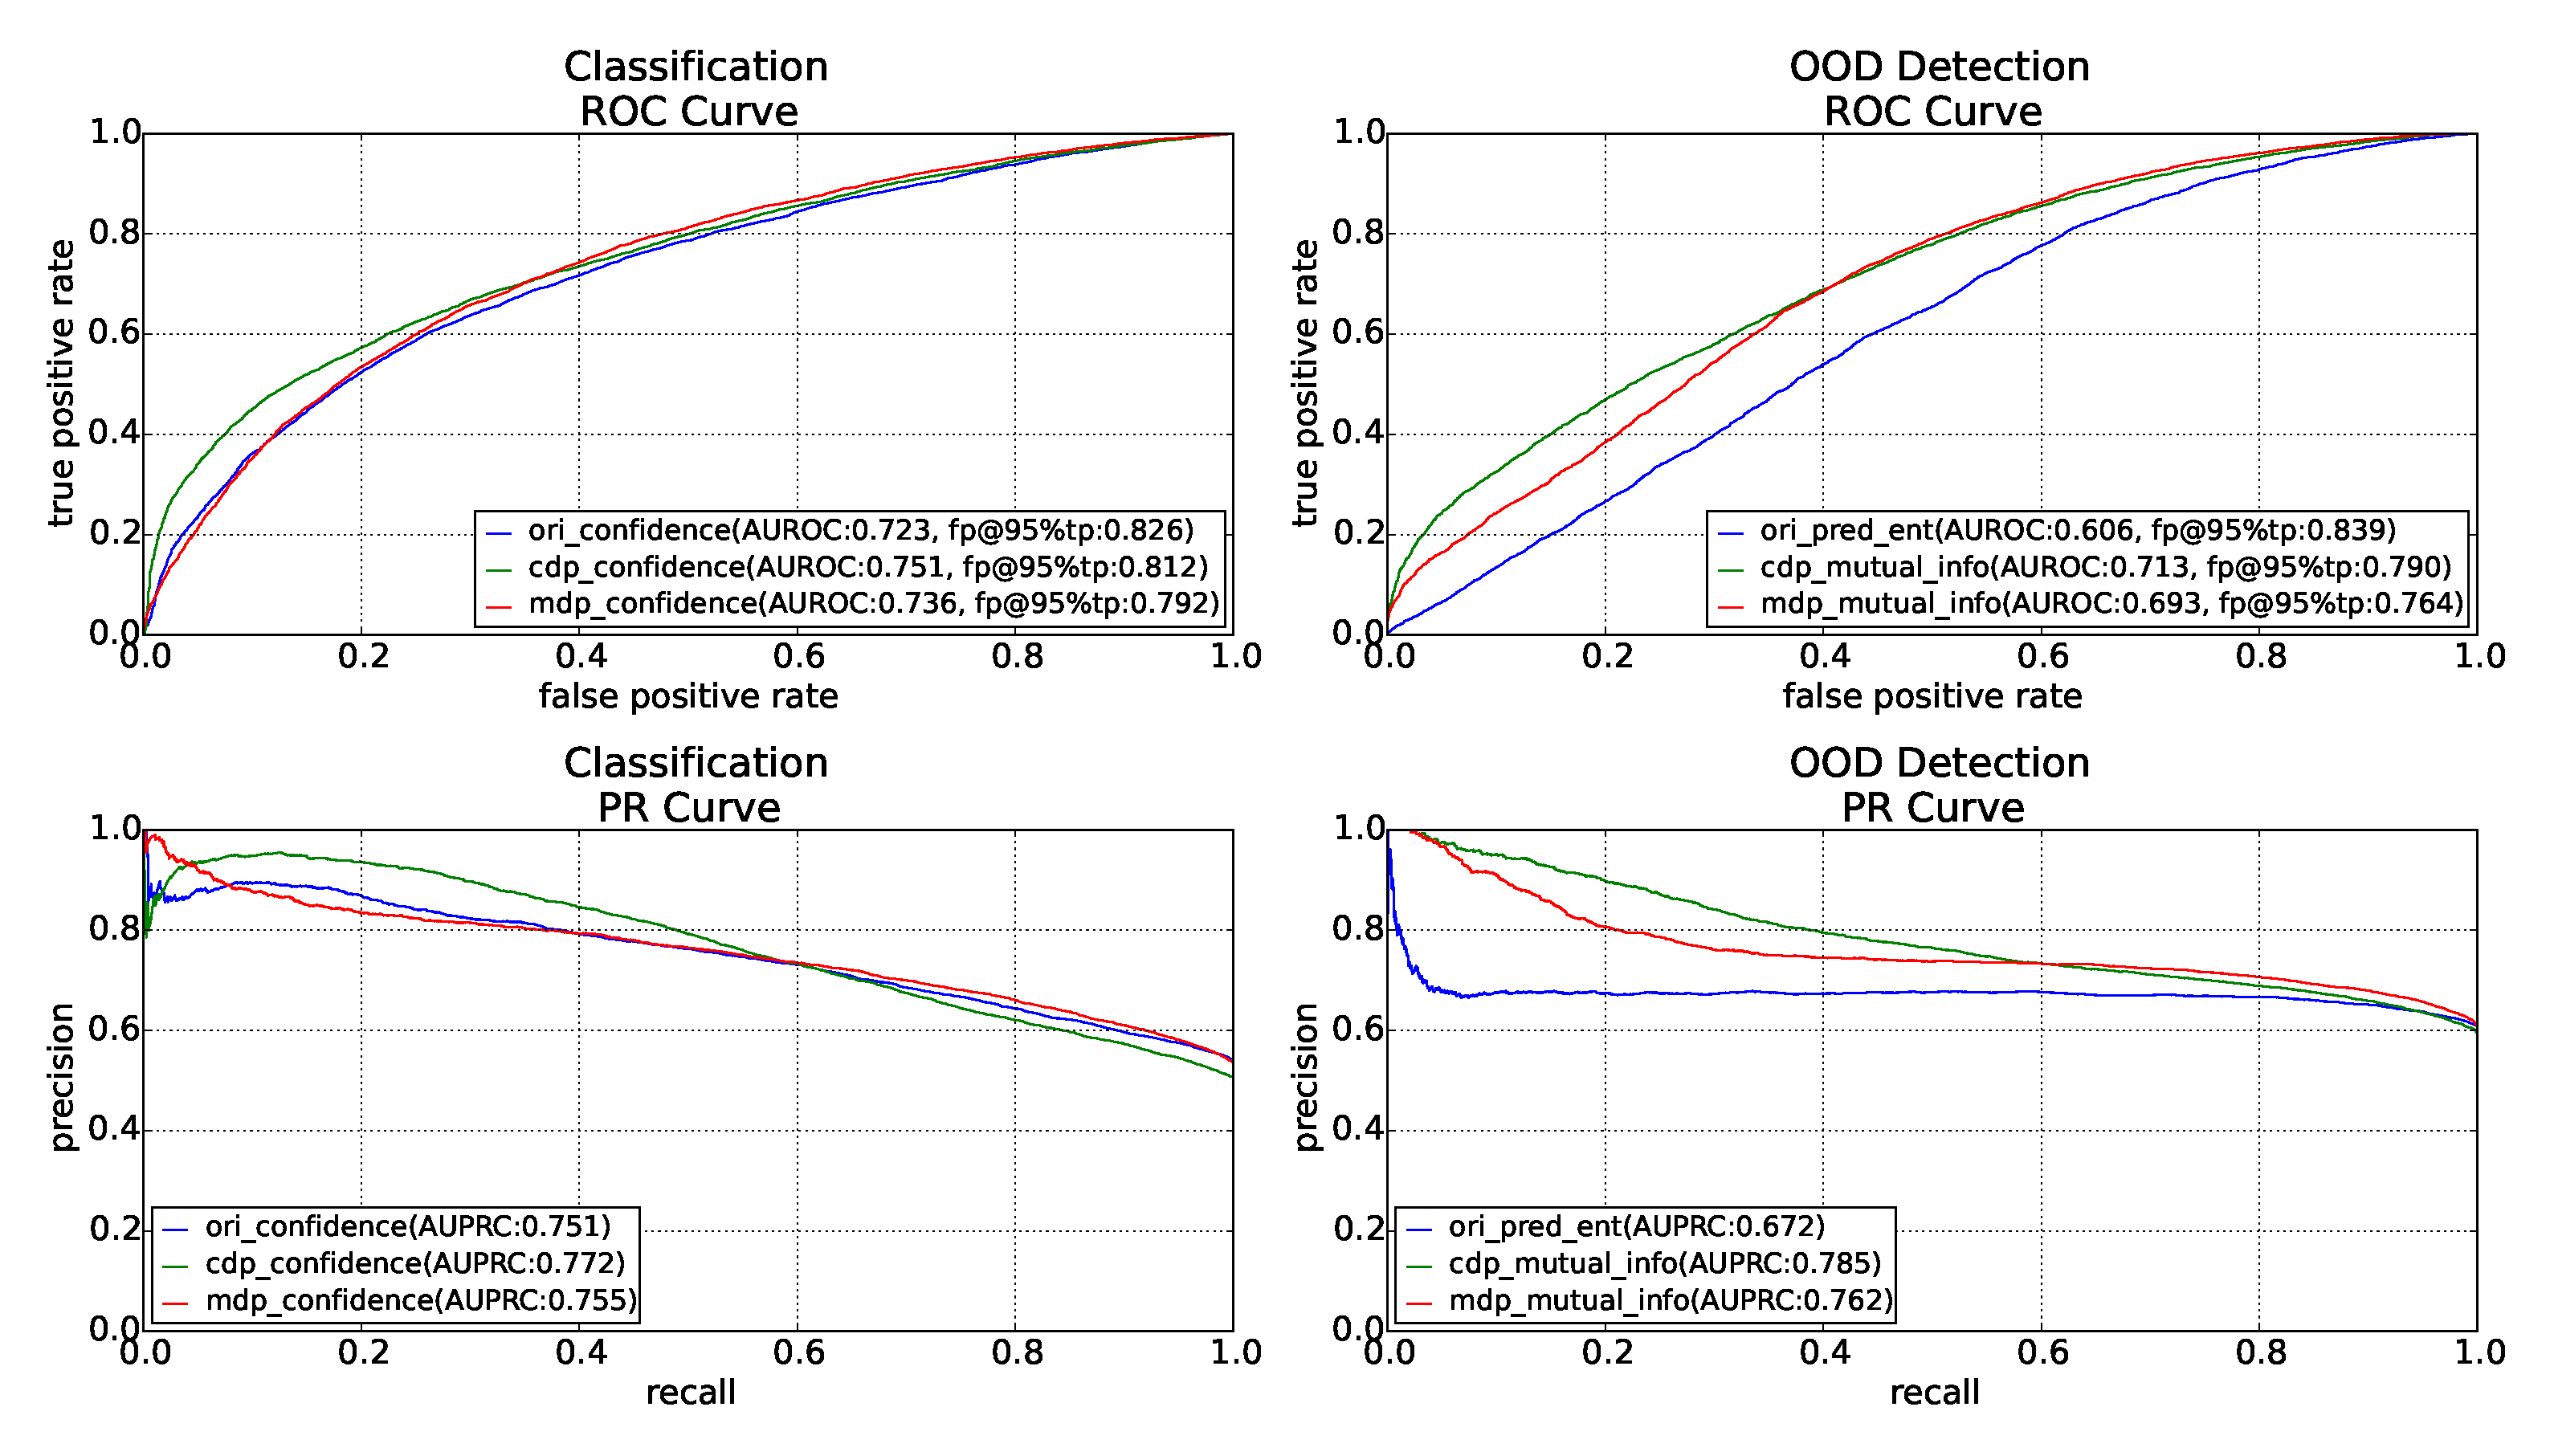
\includegraphics[height=9cm, width=16cm]{uncertainty_estimation/ablation_study/roc_pr_froFeat_ori_cdp_mdp_combined_seed3.eps}
		\caption{ROC and PR curve of one of three runs.}		
		\label{ab_roc_pr}
	\end{center}
\end{figure}
\begin{table}[H]
	\label{ab_table}
	\centering
	\caption{Quantitative results of acc, bs, nll, ece, mce, auroc, aupr.}
	\begin{tabular}{|l|l|l|l|}
		\hline
		& accuracy   $\boldsymbol \uparrow$  & brier\_score $\boldsymbol \downarrow$& \begin{tabular}[c]{@{}l@{}}negative\\ log \\ likelihood $\boldsymbol \downarrow$\end{tabular} \\ \hline
		ori           &0.532$\pm$0.015 & 0.717$\pm$0.023& 2.383$\pm$0.053                                                        \\ \hline
		cdp           & 0.521$\pm$0.011&0.655$\pm$0.017 &  2.190$\pm$0.149                                                        \\ \hline
		mdp           & 0.520$\pm$0.012 &0.641$\pm$0.014 & 1.804$\pm$0.073                                                         \\ \hline
	\end{tabular}
\end{table}

\begin{table}[H]
	\centering
	% \caption{results of ece, mce, auroc, aupr}
	\begin{tabular}{|l|l|l|l|l|}
		\hline
		& \begin{tabular}[c]{@{}l@{}}expected\\ calibration\\ error(w/o. OOD/\\ w. OOD)$\boldsymbol \downarrow$\end{tabular} & \begin{tabular}[c]{@{}l@{}}maximal\\ calibration\\ error(w/o. OOD/\\ w. OOD)$\boldsymbol \downarrow$\end{tabular} & \begin{tabular}[c]{@{}l@{}}area under\\ ROC\\ (vs. Miss-\\ classified/\\ vs. OOD)$\boldsymbol \uparrow$\end{tabular} & \begin{tabular}[c]{@{}l@{}}area under\\ PR curve\\ (vs. Miss-\\ classified/\\ vs. OOD)$\boldsymbol \uparrow$\end{tabular} \\ \hline
		ori           & \begin{tabular}[c]{@{}l@{}}0.262$\pm$0.011/ \\0.793$\pm$0.012\end{tabular}                      & \begin{tabular}[c]{@{}l@{}}0.365$\pm$0.010/ \\0.491$\pm$0.013\end{tabular}                     &
		\begin{tabular}[c]{@{}l@{}}0.716$\pm$0.005/ \\0.602$\pm$0.014\end{tabular}           & \begin{tabular}[c]{@{}l@{}}0.724$\pm$0.022/ \\0.681$\pm$0.007\end{tabular}                \\ \hline
		cdp           & \begin{tabular}[c]{@{}l@{}}0.141$\pm$0.022/ \\0.270$\pm$0.037\end{tabular}                     & \begin{tabular}[c]{@{}l@{}}0.203$\pm$0.053/ \\0.359$\pm$0.056\end{tabular}                     & \begin{tabular}[c]{@{}l@{}}0.748$\pm$0.002/ \\0.712$\pm$0.006\end{tabular}           & \begin{tabular}[c]{@{}l@{}}0.770$\pm$0.002/ \\0.782$\pm$0.004\end{tabular}                \\ \hline
		
		mdp           & \begin{tabular}[c]{@{}l@{}}0.068$\pm$0.009/ \\0.158$\pm$0.006\end{tabular}                      & \begin{tabular}[c]{@{}l@{}}0.134$\pm$0.018/ \\0.311$\pm$0.008\end{tabular}                     & \begin{tabular}[c]{@{}l@{}}0.730$\pm$0.009/ \\0.674$\pm$0.014\end{tabular}           & \begin{tabular}[c]{@{}l@{}}0.749$\pm$0.009/ \\0.748$\pm$0.010\end{tabular}                \\ \hline
	\end{tabular}
\end{table}	


\section{Automatic labeling experiments}
\subsection{Introduction}
In this experiment, our goal is to perform a proof-of-concept experiment, which simulates the situation that a classifier trained on a public large scale dataset or synthetic dataset is deployed in a real world environment and tries to fine-tune itself to improve performance wtih automatically labeled dataset and as little manually labeled data as possible. The automatically labeled data is collected based on improved uncertainty estimation. 

This way to enable the classifier to learn continuously is seldom seen in the literatures. Therefore, in order to investigate the practicability of the way, we firstly perform experiments with restriction on the size of collected dataset. 

Then we try to extend this way to another dataset to test its generalization ability in second experiment. We employ data augmentation to address the problem of imbalance in number of data sample of each category found in the first experiment and show the results.
 
\subsection{Experiments \RNum{1}}
The first experiment is performed on the WRGBD and UniHB dataset. As is mentioned in experiment \RNum{2} in uncertainty estimation, we train classifier with entire WRGBD dataset and evaluate performance of uncertainty estimation on adaptation set from UniHB dataset, which contain the images of object of elevation $30^{\circ}$ and $60^{\circ}$, whose size is around $17.1\times10^3$. The images of $45^{\circ}$ with size $8.6\times10^3$ are used for final evaluation after fine-tuning the classifier. The dataset used for fine-tuning are collected from the adaptation set with different settings in order to investigate the issues of this way for continuous learning. 

In this experiment, the model we use for fine-tuning is classifier trained with concrete dropout. The uncertainty measure we used is confidence because in this case we do not consider OOD data and confidence performs better in separating correct predictions and miss-classifications based on the results of previous experiments.

One major restriction we impose in this experiment is the size of dataset for fine-tuning. Because if we do not restrict the size, the performance is influenced by both the size of dataset and other factors such as imbalance or quality of dataset. In order to exclude the influence of dataset size, we fix it as 3\% of the adaptation set which is around 510. If the dataset is balanced in number of data sample of category, then there are around ten data samples in each category. The influence of other factors we want investigate are the imbalance of dataset and quality of data sample in dataset. In the following table, we use capital letter to denote different settings of dataset for fine-tuning.

Here we firstly illustrate the steps of labeling in this experiment which is different to the strategy in experiment \RNum{2}. 

For C, D, E, F, G, we conduct the following steps:
\begin{itemize}
	\item[1.] Automatic labeling: select the most confident predictions and label them with their predictions.
	\item[2.] Manual labeling: select the data randomly or with least confidence required for manual labeling.
	\item[3.] Combining: combine automatically labeled and manually labeled data, then check if any category does not have data sample, if yes add one random data sample of this category.
	\item[4.] Balancing dataset: firstly check if number of data sample of any categories exceed the average number of data sample (which can be calculated beforehand), if yes, drop the data sample of this category randomly until its number reach the average number of category. After that, if augmentation is chosen, then use augmentation to increase of the number of data sample of category in which the number of data sample is less than average number of data sample.

\end{itemize}
To note that, the accuracy of automatically labeled data in C, E, F, G is around 96\%, which means not all labels of them are correct. And "\textbf{randomly}" in the settings means that we randomly choose the data according to the number of data sample in each category in order to make the dataset \textbf{as balanced as possible}.  
\begin{table}[H]
	\centering
	\label{table:fine_tuning}
	\caption{Results of fine-tuning of different settings}
	\begin{tabular}{|l|c|}
		\hline
		Settings of dataset for fine-tuning                                                                                                                                                                                   & \multicolumn{1}{l|}{\begin{tabular}[c]{@{}l@{}}Accuracy\\ (average over 3\\ random seeds)\end{tabular}} \\ \hline
		A: 0\% (no fine-tuning)                                                                                                                                                                                                  & 66.9\%                                                                                                  \\ \hline
		\begin{tabular}[c]{@{}l@{}}B: 3\% manually labeled data randomly \\   (\textbf{balanced})\end{tabular}                                                                                                                               & 91.7\%                                                                                                  \\ \hline
		\begin{tabular}[c]{@{}l@{}}C: 3\% automatically labeled data \\ (\textbf{imbalanced})\end{tabular}                                                                                                                        & 79.0\%                                                                                                  \\ \hline
		\begin{tabular}[c]{@{}l@{}}D: 3\% manually labeled data with least confidence\\ (\textbf{imbalanced})\end{tabular}                                                                                                       & 83.3\%                                                                                                  \\ \hline
		\begin{tabular}[c]{@{}l@{}}E: 2\% automatically labeled data and \\ 1\% manually labeled data with least confidence, \\ augmentation for balance (\textbf{balanced})\end{tabular}                                     & 83.8\%                                                                                                  \\ \hline
		\begin{tabular}[c]{@{}l@{}}F: 2\% automatically labeled data and \\ 0.5\% manually labeled data with least confidence and \\ 0.5\% manually labeled data randomly,\\ augmentation for balance (\textbf{balanced})\end{tabular} & 88.3\%                                                                                                  \\ \hline
		\begin{tabular}[c]{@{}l@{}}G: 2\% automatically labeled data and \\ 1\% manually labeled data randomly,\\ augmentation for balance (\textbf{balanced})\end{tabular}                                                            & 89.6\%                                                                                                  \\ \hline
	\end{tabular}
\end{table}
From the description of settings we know that predictions with most confidence and least confidence are imbalanced in number of data sample of each category.Based on the results in the table above, we can have the following observations:
\begin{itemize}
	\item diverse and balanced dataset can achieved best performance.
	\item the difference of performance between C and D may attribute to quality of dataset which include correct labeling and information of data sample.
	\item by comparing performance of E, F and G, we know that diverse data sample before augmentation is important to achieve better performance. When considering information of data sample, manually labeling of lest confident data sample sounds better. However, we also know that before augmentation dataset in E is more imbalanced than that in F, and F is more imbalanced than G because of the higher proportion of predictions with least confidence. Therefore it shows that data balance is more important than information of data sample in this case.
\end{itemize}
By comparing the results of other settings with that of A and B, we can see that the manual labeling effort can be reduced based on automatic labeling.  The performance of fine-tuned domain specific classifier can nearly reach the the performance of classifier fine-tuned with all manually labeled data. 

In the end, we can also draw a conclusion that diversity of data and balance of number of data sample of each category play an significant role. Based on the last aforementioned observation, balance of number of data sample of each category is more important in than information of data sample.

\subsection{Experiments \RNum{2}}
The second experiment is performed on synthetic Tless dataset and original Tless dataset.


\section{Context-based improvement experiments}
\subsection{Experiments settings}
\subsection{Results}
\subsection{Analysis}
%\include{Results}
%  Conclusions (Zusammenfassung):
\chapter{Conclusion}
\subsection{Discussions and conclusions}

\begin{itemize}
	\item 
\end{itemize}


\subsection{Future work}
\begin{itemize}
	\item check uncertainty distribution of different view points of the object.
	\item try distillation method to decrease runtime of testing.
	\item try more complex and expressive approximate posterior distribution such as normalizing flow.
	\item improve performance of multiple dropout.
\end{itemize}
% Appendix (Anh�nge), could have multiple chaper-files:
\appendix
\chapter{Appendix}
% \section{KL condition}
% \label{appendix:kl_condition}
% \paragraph{Proposition} Fix $K$, $L \in \mathbb N$, a probability vector $\bld p = (p_{1}, ..., p_{L})$, and $\bld \Sigma_{i} \in \mathbb R^{K \times K}$ diagonal positive definite for $i=1,...,L$, with the elements of each $\bld \Sigma_{i}$ not dependent on $K$. Let
%\[
%q(\bld x) = \sum_{i=1}^{L} p_{i}\mathcal N(\bld x; \bld \mu_{i}, \bld \Sigma_{i}) 
%\]
%be a mixture of Gaussians with $L$ components and $\bld \mu_{i} \in \mathbb R^{K}$, let $p(\bld x) = \mathcal N(0, \bld I_{K})$, and further assume that $\bld \mu_{i} - \bld \mu_{j} \sim \mathcal N(0, \bld I)$ for all $i$ and $j$.
%
%The KL divergence between $q(\bld x)$ and $p(\bld x)$ can be approximated as:
%\[ 
%KL(q(\bld x) || p(\bld x)) \approx \sum_{i=1}^{L}\frac{p_{i}}{2}(\bld \mu_{i}^{T} \bld \mu_{i} + tr(\bld \Sigma_{i}) - K(1+\text{log}2\pi) - \text{log}(\text{det}(\bld \Sigma_{i}))) - \mathcal H (\bld p)
%\] 
%with 
%\[
%\mathcal H(\bld p) = -\sum_{i=1}^{L}p_{i}\text{log}p_{i}
%\]
%for large enough $K$. 
%
%\paragraph{$Proof.$}
%We have 
%\[
%\begin{aligned}
%KL(q(\bld x) || p(\bld x)) &= \int q(\bld x) \text{log }\frac{q(\bld x)}{p(\bld x)} d\bld x \\
%&=\int q(\bld x) \text{log} q(\bld x) d\bld x - \int q(\bld x)\text{log} p(\bld x) d\bld x \\
%&=-\mathcal H(q(\bld x)) - \int q(\bld x)\text{log } p(\bld x) d\bld x 
%\end{aligned}
%\]
%which is sum of entropy of $q(\bld x)$ and the expected log probability of $\bld x$. The expected log probability can be evaluated analytically, but the entropy term has to be approximated.
%
%We begin by approximating the entropy term. We write 
%\[
%\begin{aligned}
%\mathcal H(q(\bld x)) &= -\sum_{i=1}^{L}p_{i}\int \mathcal N(\bld x; \bld \mu_{i}, \bld \Sigma_{i})\text{log }q(\bld x)d\bld x \\
%&=-\sum_{i=1}^{L} p_{i}\int \mathcal N(\bld \epsilon_{i}; 0, \bld I) \text{log } q(\bld \mu_{i} + \bld L_{i} \bld \epsilon_{i}) d\bld \epsilon_{i} \\ 
%\end{aligned}
%\] 
%with a re-parameterization of $\bld x$, that is $\bld x = \bld \mu_{i} + \bld L_{i} \bld \epsilon_{i}$ with $\bld L_{i} \bld L_{i}^{T} = \bld \Sigma_{i}$ and $\bld \epsilon_{i} \sim \mathcal N(0, I)$.
%
%Now the term inside logarithm can be written as 
%\[
%\begin{aligned}
%q(\bld \mu_{i} + \bld L_{i}\bld \epsilon_{i}) &= \sum_{j=1}^{L} p_{j} \mathcal N(\bld \mu_{i}+\bld L_{i}\bld \epsilon_{i}; \bld \mu_{j}, \bld \Sigma_{j}) \\
%&=\sum_{j=1}^{L}p_{j}(2\pi)^{-\frac{K}{2}} \text{det}(\bld \Sigma_{j})^{-\frac{1}{2}}\text{exp }\{-\frac{1}{2}||\bld \mu_{j} - \bld \mu_{i} - \bld L_{i} \bld \epsilon_{i}||^{2}_{\bld \Sigma_{j}}\}
%\end{aligned}
%\]
%where $||\cdot||_{\bld \Sigma}$ is Mahalanobis distance with $\bld \Sigma$ as covariance matrix. Since $\bld \mu_{i} - \bld \mu_{j}$ is assumed to be normally distributed, the quantity $\bld \mu_i - \bld \mu_{j} - \bld L_{i} \bld \epsilon_{i} $ is also normally distributed. Since the expectation of a generalized $\mathcal X^{2}$ distribution with $K$ degrees of freedom increases with $K$, we have that $K \gg 0$ implies that $||\bld \mu_i - \bld \mu_{j} - \bld L_{i} \bld \epsilon_{i} ||^{2}_{\bld \Sigma_{j}} \gg 0 $ for $i \neq j$(since the elements of $\bld \Sigma_{j}$ does not depend on $K$). Finally, we have for $i=j$ that  $||\bld \mu_i - \bld \mu_{j} - \bld L_{i} \bld \epsilon_{i} ||^{2}_{\bld \Sigma_{j}} = \bld \epsilon_{i}^{T} \bld L_{i}^{T} \bld L_{i}^{-T} \bld L_{i}^{-1} \bld L_{i} \bld \epsilon_{i} = \bld \epsilon_{i}^{T} \bld \epsilon_{i}$. Therefore the last equation can be approximated as 
%\[
%q(\bld \mu_{i} + \bld L_{i} \bld \epsilon_{i}) \approx p_{i}(2\pi)^{-\frac{K}{2}}\text{det}(\bld \Sigma_{i})^{-\frac{1}{2}}\text{exp }\{-\frac{1}{2}\bld \epsilon_{i}^{T} \bld \epsilon_{i}\}
%\]
%I.e. in high dimensions the mixture components will not overlap.This gives us 
%\[
%\begin{aligned}
%\mathcal H(q(\bld x)) & \approx -\sum_{i=1}^{L} p_{i}\int \mathcal N(\bld \epsilon_{i}; 0, \bld I) \text{log } \big(p_{i}(2\pi)^{-\frac{K}{2}}\text{det}(\bld \Sigma_{i})^{-\frac{1}{2}}\text{exp }\{-\frac{1}{2}\bld \epsilon_{i}^{T} \bld \epsilon_{i}\}\big) d\bld \epsilon_{i} \\ 
%&= -\sum_{i=1}^{L}p_{i}\big[\text{log }p_{i} - \frac{K}{2}\text{log }2\pi  - \frac{1}{2} \text{log }\text{det}(\bld \Sigma_{i}) - \frac{1}{2}\int \mathcal N(\bld \epsilon_{i}; 0, \bld I)\bld \epsilon_{i}^{T} \bld \epsilon_{i} d \bld \epsilon_{i}\big] \\
%&=\sum_{i=1}^{L}\frac{p_{i}}{2}\big(K\text{log }2\pi + \text{log } \text{det}(\bld \Sigma_{i}) + \int \mathcal N(\bld \epsilon_{i};0, \bld I)\bld \epsilon_{i}^{T}\bld \epsilon_{i}d\bld \epsilon_{i} \big) + \mathcal H(\bld p)
%\end{aligned}
%\] 
%Since $\bld \epsilon_{i}^{T}\bld \epsilon_{i}$ distributes according to a $\mathcal X^{2}$ distribution , its expectation is $K$, and in the end the entropy term can be approximated as 
%\[
%\mathcal H(q(\bld x)) \approx \sum_{i=1}^{L}\frac{p_{i}}{2}\big(K(\text{log }2\pi + 1) + \text{log } \text{det}(\bld \Sigma_{i}) \big) + \mathcal H(\bld p)
%\]
%
%Next, we can evaluate the expected log probability term, we get 
%\[
%\int q(\bld x) \text{log }p(\bld x) d\bld x = \sum_{i=1}^{L}p_{i}\int \mathcal N(\bld x; \bld \mu_{i}, \bld \Sigma_{i})\text{log }p(\bld x) d\bld x
%\]
%for $p(\bld x) = \mathcal N(0, \bld I_{K})$, it is easy to show that
%\[
%\begin{aligned}
%\int q(\bld x) \text{log }p(\bld x) d\bld x &= \sum_{i=1}^{L}p_{i} \int 
%\mathcal N(\bld x; \bld \mu_{i}, \bld \Sigma_{i}) \text{log}\big[(2\pi)^{-\frac{K}{2}} \text{det}(\bld I_{K})^{-\frac{1}{2}} \text{exp}\{-\frac{1}{2}\bld x^{T} \bld x \} \big] d\bld x \\ 
%&= \sum_{i=1}^{L}p_{i} \big[
%-\frac{K}{2} \text{log} 2\pi
%-\frac{1}{2}\int \mathcal N(\bld x; \bld \mu_{i}, \bld \Sigma_{i}) \bld x^{T} \bld x d\bld x
%\big]\\
%&=-\frac{1}{2}\sum_{i=1}^{L}p_{i}(\bld \mu_{i}^{T} \bld \mu_{i} + tr(\bld \Sigma_{i}) + K\text{log}2\pi)
%\end{aligned}
%\]
%
%Finally, combining the equations above, we have 
%\[ 
%KL(q(\bld x) || p(\bld x)) \approx \sum_{i=1}^{L}\frac{p_{i}}{2}(\bld \mu_{i}^{T} \bld \mu_{i} + tr(\bld \Sigma_{i}) - K - \text{log}(\text{det}(\bld \Sigma_{i}))) - \mathcal H (\bld p)
%\] 
%as required to show.  
%\begin{flushright}
%	$\square$
%\end{flushright}

\section{Fisher information} \label{appendix:fisher_matrix}
Here, we consider the case that parameter of likelihood function is scalar. This can easily be extended to the case that $\theta$ is a vector. Fisher information $\mathcal{I}(\theta)$ is defined as follows:
\begin{equation}
	\mathcal{I}(\theta) = \mathbb{E}\big[\big(\frac{\partial}{\partial \theta}\log{f(X; \theta)}\big)^2\big]
\end{equation}
Where $f(X;\theta)$ is probability density function or mass function of random variable $X$. We need to prove that $\mathbb{E}\big[\big(\frac{\partial}{\partial \theta}\log{f(X; \theta)}\big)^2\big] = \mathbb{E}\big[-\frac{\partial^2}{\partial \theta^2}\log{f(X; \theta)}\big]$.
When we suppose that $\theta$ is the true parameter. Based on the fact that $f(X;\theta)$ is density, we can have:
\[
\int f(x;\theta) dx = 1
\]
Differentiating the above with respect to $\theta$ gives:
\[
\frac{\partial}{\partial \theta}\int f(x;\theta) dx = 0
\]
After moving differentiating operation into integration and making use of derivative of logarithm, we get:
\[
\int \frac{\partial \log f(x;\theta)}{\partial \theta} f(x;\theta) dx = 0
\]
Differentiating again w.r.t. $\theta$ and taking the derivative inside gives:
\[
\begin{aligned}
&\int \frac{\partial^2\log f(x;\theta)}{\partial \theta^2}f(x;\theta) dx + \int \frac{\partial\log f(x;\theta)}{\partial \theta} \frac{\partial f(x;\theta)}{\partial \theta}dx
= 0\\
\Rightarrow &\int \frac{\partial^2\log f(x;\theta)}{\partial \theta^2}f(x;\theta) dx + \int \frac{\partial\log f(x;\theta)}{\partial \theta} \frac{\partial f(x;\theta)}{\partial \theta}\frac{1}{f(x;\theta)} f(y;\theta) dx= 0 \\
\Rightarrow &\int \frac{\partial^2\log f(x;\theta)}{\partial \theta^2}f(x;\theta) dx + \int \frac{\partial\log f(x;\theta)}{\partial \theta} \frac{\partial \log f(x;\theta)}{\partial \theta} f(y;\theta) dx= 0 \\
\Rightarrow & -\mathbb{E}[\frac{\partial^2\log f(x;\theta)}{\partial \theta^2}] = \mathbb{E}[\frac{\partial\log f(x;\theta)}{\partial \theta} \frac{\partial \log f(x;\theta)}{\partial \theta} ] \\
\end{aligned}
\]
which gives us the required result.
 \begin{flushright}
 	$\square$
 \end{flushright}
 
%\section{Implementation details}



% List of figures (Abbildungsverzeichnis):
\listoffigures
% List of tables (Tabellenverzeichnis):
\listoftables
% Glossary (Glossar):
%\include{Glossary}
% List of formulae (Liste der Formelzeichen):
%\include{Formulae}
% Abbreviations (Abk�rzungsverzeichnis):
%\include{Abbreviations}

% References (Literaturverzeichnis):
% a) Style (with numbers: use unsrt, otherwise:alpha):
\bibliographystyle{alpha}
% b) The File:
\bibliography{Bibliography}

\end{document} %*****************************************************
